
%!TEX TS-program = lualatex
%!TEX encoding = UTF-8 Unicode


%\documentclass[11pt,b5paper]{book}
% \usepackage{fontspec}
% \defaultfontfeatures{Mapping=tex-text}
%\usepackage{amsmath}
%\usepackage{amssymb}
%\usepackage{euler}
%		\usepackage{geometry}
% setting page parameters
%		\geometry{textwidth=5in, textheight=7.5in,  marginparsep=7pt, marginparwidth=.6in}
%\usepackage{longtable}
\documentclass[10pt]{scrbook}
\usepackage{geometry}                % See geometry.pdf to learn the layout options. There are lots.
\geometry{paperheight=150mm,paperwidth=150mm, textwidth=75mm, textheight=100mm,                 top=20mm, bottom=20mm, marginparwidth=38mm, headsep=8mm, left=10mm, right=55mm, marginparsep=7mm, footskip=10mm}                   % ... or a4paper or a5paper 
% ... or a4paper or a5paper or ... 
%\geometry{landscape}                % Activate for for rotated page geometry
%\usepackage[parfill]{parskip}    % Activate to begin paragraphs with an empty line rather than an indent
%\usepackage[]{euler}
\usepackage{graphicx}
%\usepackage[]{gfsneohellenic}
\usepackage{amsmath}

\usepackage{amssymb}

%\usepackage[sfdefault]{josefin}
\usepackage[libertine]{newtxmath}
\usepackage[nomath]{libertinus}

\usepackage{marginnote}
\usepackage{sidenotes}
\renewcommand*{\marginfont}{\footnotesize}
\renewcommand\raggedrightmarginnote{}
\renewcommand\raggedleftmarginnote{}

\makeatletter
\ExplSyntaxOn
\RenewDocumentCommand \@sidenotes@placemarginal { m m }
{
  \IfNoValueOrEmptyTF{#1}
    % substitue \marginnote from marginnote pkg for \marginpar 
    % from latex2e format
    {\marginnote{#2}}
    {\marginnote{#2}[#1]}
}
\ExplSyntaxOff
\makeatother
%https://tex.stackexchange.com/questions/532245/how-to-modify-fonts-in-sidenotes

\usepackage{soul}
\usepackage[tracking=smallcaps,letterspace=100]{microtype}


\addtokomafont{chapter}{\color{darkgray}}
\addtokomafont{section}{\color{gray}}
\addtokomafont{subsection}{\color{LightSlateGray}}
\setkomafont{caption}{\small\sffamily}

\setlength{\textfloatsep}{0.9\baselineskip plus 0.2\baselineskip minus 0.5\baselineskip}

\RedeclareSectionCommand[beforeskip=.5\textheight plus 1.25\baselineskip]{chapter}

\newcommand{\ans}{\marginnote{\textcolor{SteelBlue}{{\large \emph{Answer}}}}}% prints in red

\newcommand{\ques}{\marginnote{\textcolor{Salmon}{{\large \emph{Question}}}}}% prints in red

\newcommand{\drkgry}[1]{\textcolor{darkgray}{{#1}}}

% Redefine \partpagestyle to empty
\renewcommand*{\partpagestyle}{empty}

\usepackage[per-mode=symbol]{siunitx}
\sisetup{
  group-separator={,},
  group-minimum-digits=4,
}

%\usepackage{concmath}
%\usepackage{kpfonts}
\usepackage{enumitem}
\usepackage[usenames,dvipsnames,svgnames,table]{xcolor}

% \usepackage{colortbl}
\usepackage{multicol}
\usepackage{mathtools}

\usepackage{graphicx}


% for numbers/text with circles around them
% hyper referencing objects urls etc
\usepackage[colorlinks = true, urlcolor=DodgerBlue, linkcolor=darkgray, citecolor=DodgerBlue,linktoc=all]{hyperref}


\RedeclareSectionCommand[
  runin=false,
  afterindent=false,
  beforeskip=.5\baselineskip,
  afterskip=5pt]{section}
  
%\usepackage{basicarith}
%\usepackage{xlop}
% Adjust the space after floats
% Define a new command for easier spacing adjustment

\newcommand*\figr[1]{\hyperref[#1]{Figure~\ref{#1}}}

\usepackage{emptypage}

\usepackage{epigraph}

%\usepackage{tikz}

\usepackage{physics}
\usepackage{pdfpages}

%%%%%%  END OF PACKAGES 

\title{Geometry for Entertainment}
\author{Yakov Perelman}
\date{2024}
%%%% META DATA

\begin{document}
\renewcommand{\baselinestretch}{1}\normalsize

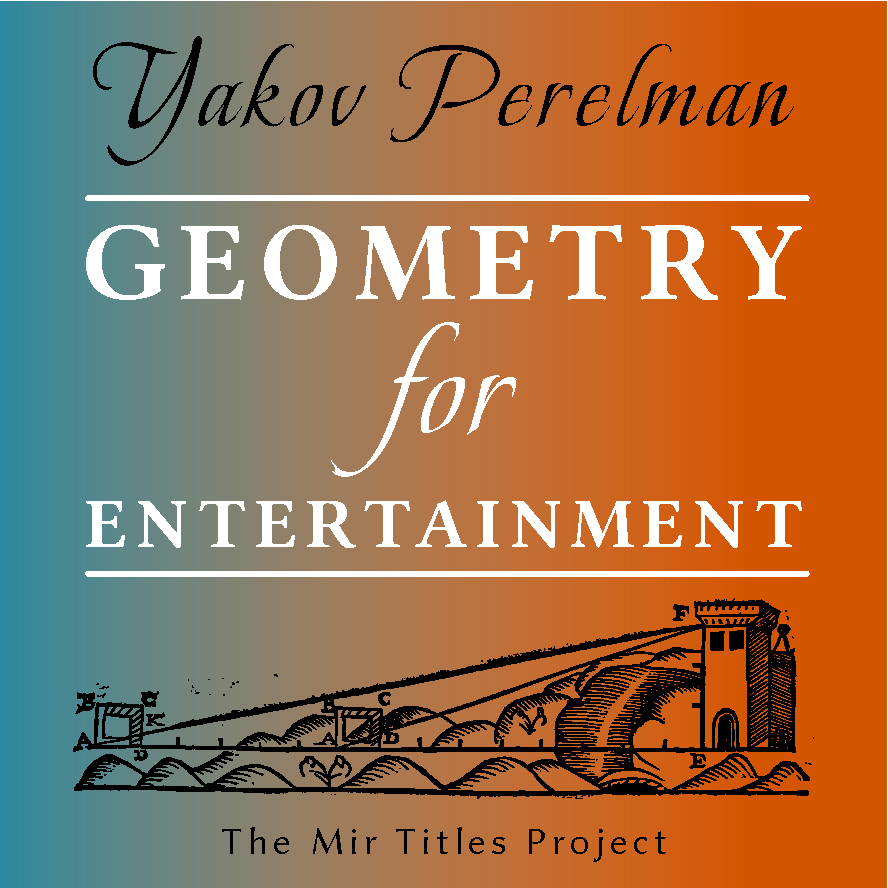
\includepdf{figures/perelman-geometry-fc.pdf}

\frontmatter

% !TEX root = perelman-geometry.tex
%!TEX TS-program = pdflatex
%!TEX encoding = UTF-8 Unicode


\maketitle
\cleardoublepage
\thispagestyle{empty}
%\pagenumbering{roman}
\begin{center}

{\LARGE Ya. I. Perelman}

{\Huge Geometry for Entertainment}




The Mir Titles Project

\end{center}
\cleardoublepage

\thispagestyle{empty}
\vfill

{\noindent
Seventh Edition, Revised

Edited and supplemented by B. A. Kordemsky

First Published by State Publishing House Of Technical And Theoretical Literature Moscow -- 1950 -- Leningrad.

Original scan in Russian by the Russian Lutherean on The Internet Archive \url{https://archive.org/details/20220910_perelman_geometry/}.

Translated from the Russian and typeset in \LaTeX{} by \emph{Damitr Mazanav}.

This fully electronic English translation released on the web by \emph{The Mir Titles Project}. \url{https://mirtitles.org} in 2024.

 


Licence Creative Commons by SA 4.0

\cleardoublepage

 \tableofcontents
 
 \cleardoublepage

\chapter{Editor's Preface}
\label{editor-preface}
%\addcontentsline{toc}{chapter}{\nameref{preface}}


\emph{Geometry for Entertainment} is written both for friends of mathematics and for those readers from whom many attractive aspects of mathematics have somehow been hidden.

More importantly, this book is intended for those readers who studied (or are currently studying) geometry only at the blackboard and therefore are not used to noticing familiar geometric relationships in the world of things and phenomena around us, have not learnt to use the acquired geometric knowledge in practise, in difficult cases of life, on a hike, in a bivouac or front-line situation.

To arouse the reader's interest in geometry or, in the words of the author, ``to inspire a desire and cultivate a taste for its study is the objective of this book.''

To this end, the author will take geometry ``out of the walls of the school room into the free air, into the forest, field, to the river, on the road, in order to indulge in relaxed geometric studies without a textbook and tables in the open air \ldots{}'', and draws the reader's attention to the pages of L. N. Tolstoy and A. P. Chekhov, Jules Verne and Mark Twain. He finds a theme for geometric problems in the works of N. V. Gogol and A. S. Pushkin, and finally offers the reader ``a motley selection of problems, curious in plot, unexpected in result.''

The seventh edition of \emph{Geometry for Entertainment} is published without the direct participation of the author. Ya. I. Perelman died in Leningrad in 1942.

The new edition of the book contains almost all the articles of the previous edition, newly illustrated, edited and supplemented with facts and information from our Soviet reality, as well as a considerable number (about 30) additional articles.

I was guided by the desire to increase the ``utility coefficient'' of Ya. Perelman's book, to make it even more effective and interesting, involving new readers in the ranks of friends of mathematics.

To what extent this was possible, I hope to learn from readers at the address: Moscow, 64, Chernyshevsky Str., 81, Sq. 53, B. A. Kordemsky.


\begin{flushright}
\emph{B. Kordemsky}
\end{flushright}


\chapter{Translator's Preface}
\label{translator-preface}
%\addcontentsline{toc}{chapter}{\nameref{preface}}

Yakov Perelman's books have been a constant source of inspiration for me throughout my life. It brings me great pleasure to present this as of now untranslated work of Perelman to English world. 

I have tried my level best to create a readable version of the translation. If there are any mistakes they are all mine. Any suggestions and criticisms to improve the translation are welcome. I hope that this English version finds enthusiastic readers.

\begin{flushright}
\emph{Damitr Mazanav}
\end{flushright}



\mainmatter

\part{Geometry In The Open Air}

% !TEX root = perelman-geometry.tex
%!TEX TS-program = pdflatex
%!TEX encoding = UTF-8 Unicode

% epigraph for part 1

\cleardoublepage
\vspace*{\fill}
\begin{center}
\epigraph{\begin{minipage}{0.4\pagewidth} \textsf{Nature speaks the language of mathematics: the letters of this language are circles, triangles and other mathematical shapes.}\end{minipage}}{Galileo}
\end{center}
\vspace*{\fill}

\thispagestyle{empty}

% begin chapter

\cleardoublepage

%\RedeclareSectionCommand[beforeskip=2.75cm]{chapter}
%\RedeclareSectionCommand[afterskip=1cm]{chapter}
%\RedeclareSectionCommand[beforeskip=0.1\baselineskip,afterskip=0.25\baselineskip]{section}
%
%\RedeclareSectionCommand[beforeskip=-1cm]{section}
%\vspace*{2cm} % Adjust the value as needed

\setchapterpreamble[o]{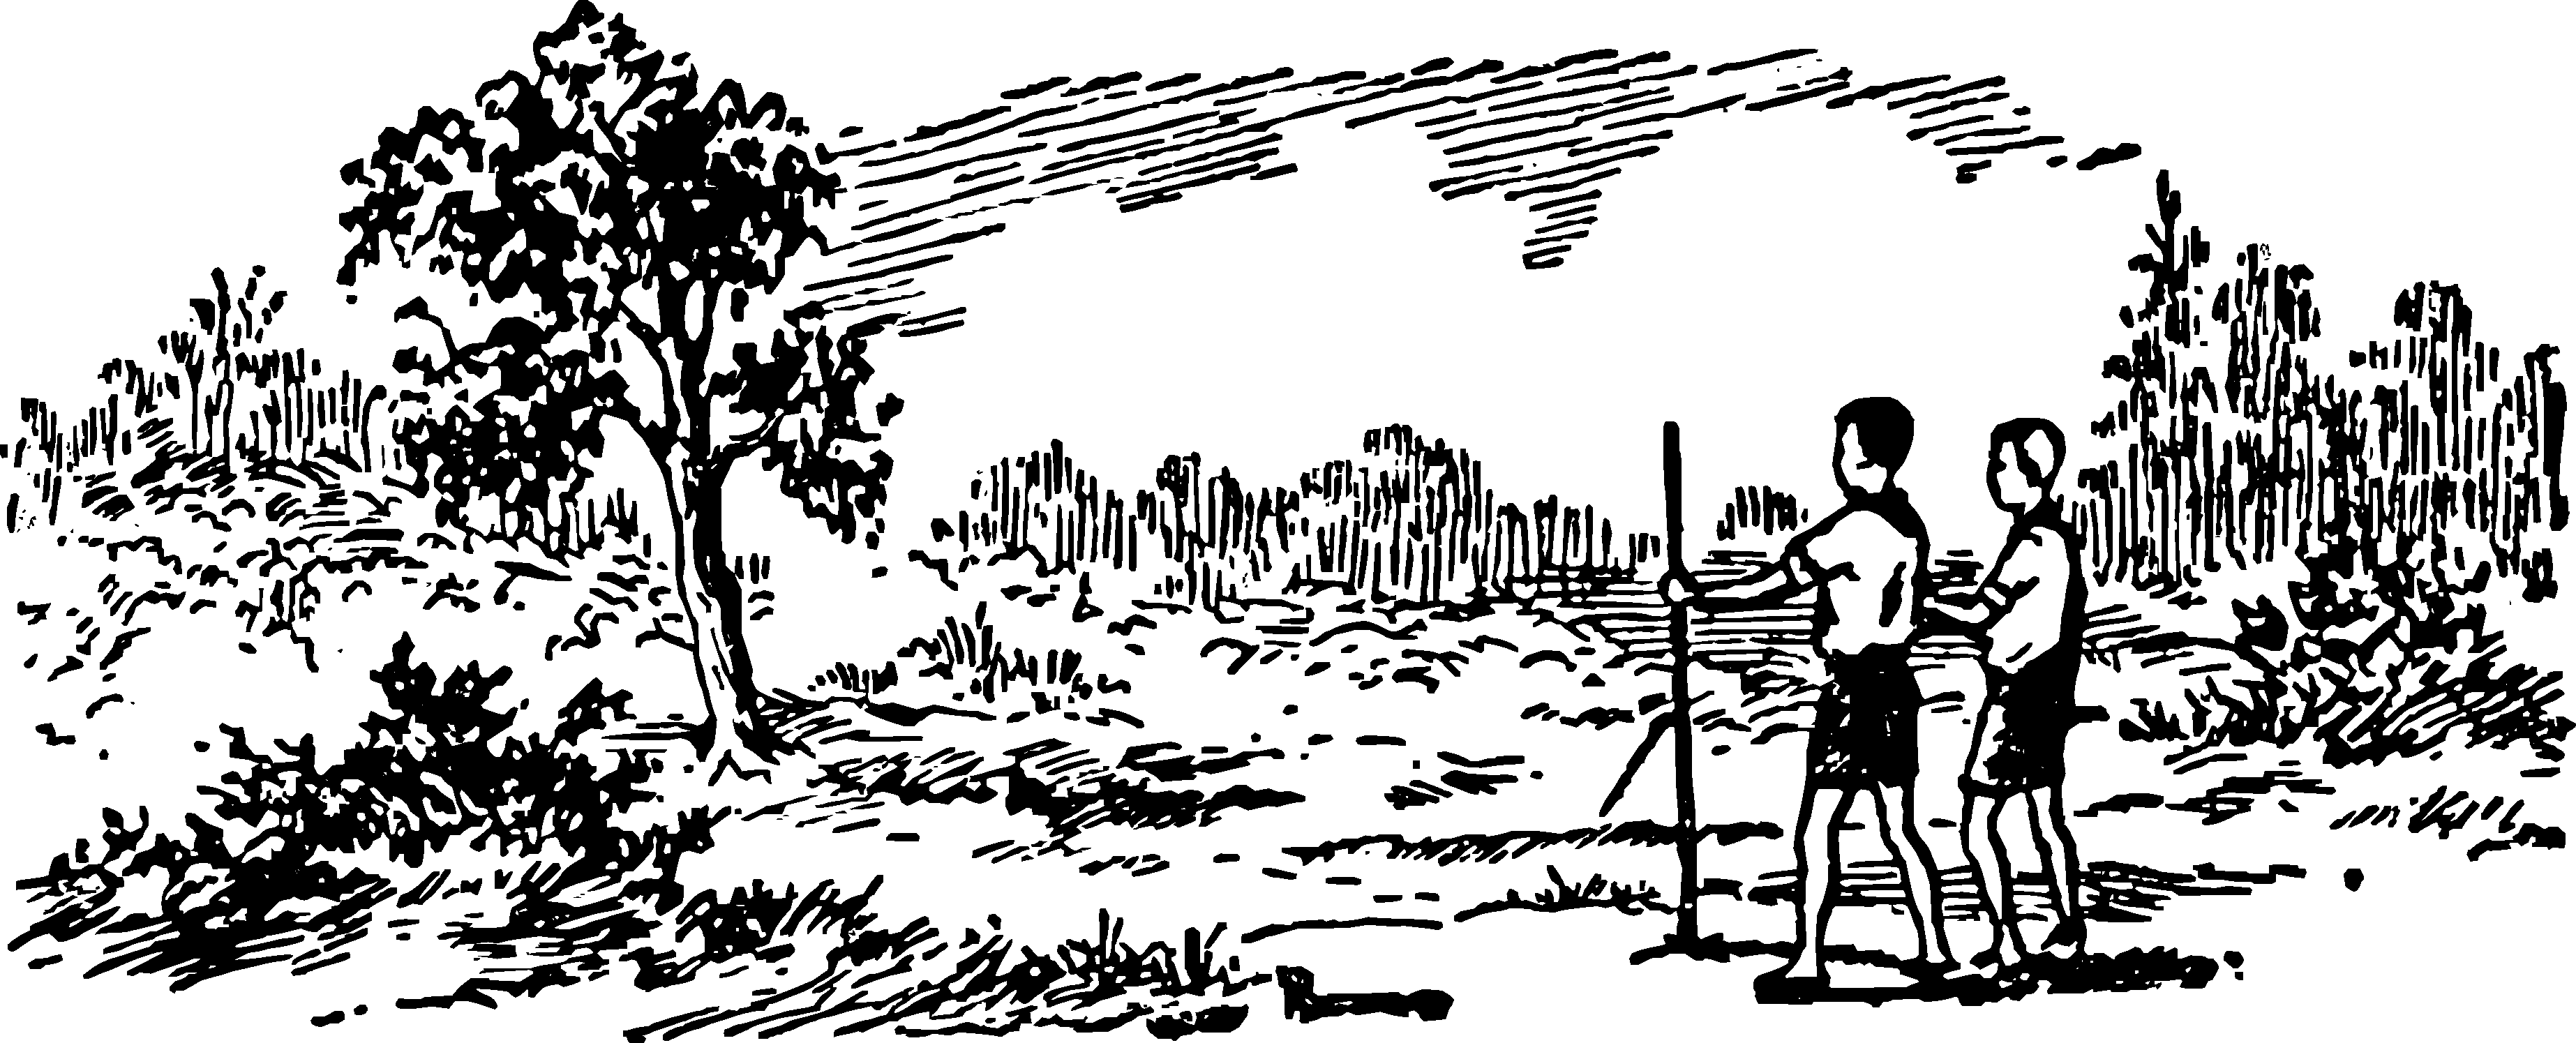
\includegraphics[width=1.2\textwidth]{figures/ch-01/fig-ch-01-head.pdf}\bigskip}

\chapter{Geometry In The Forest}
\label{ch-01}

%\begin{tikzpicture}[remember picture,overlay,shift=(current page.north west)]
%\begin{scope}[x={(current page.north east)},y={(current page.south west)}]
%\node [overlay,remember picture] at (0.5,0.2) {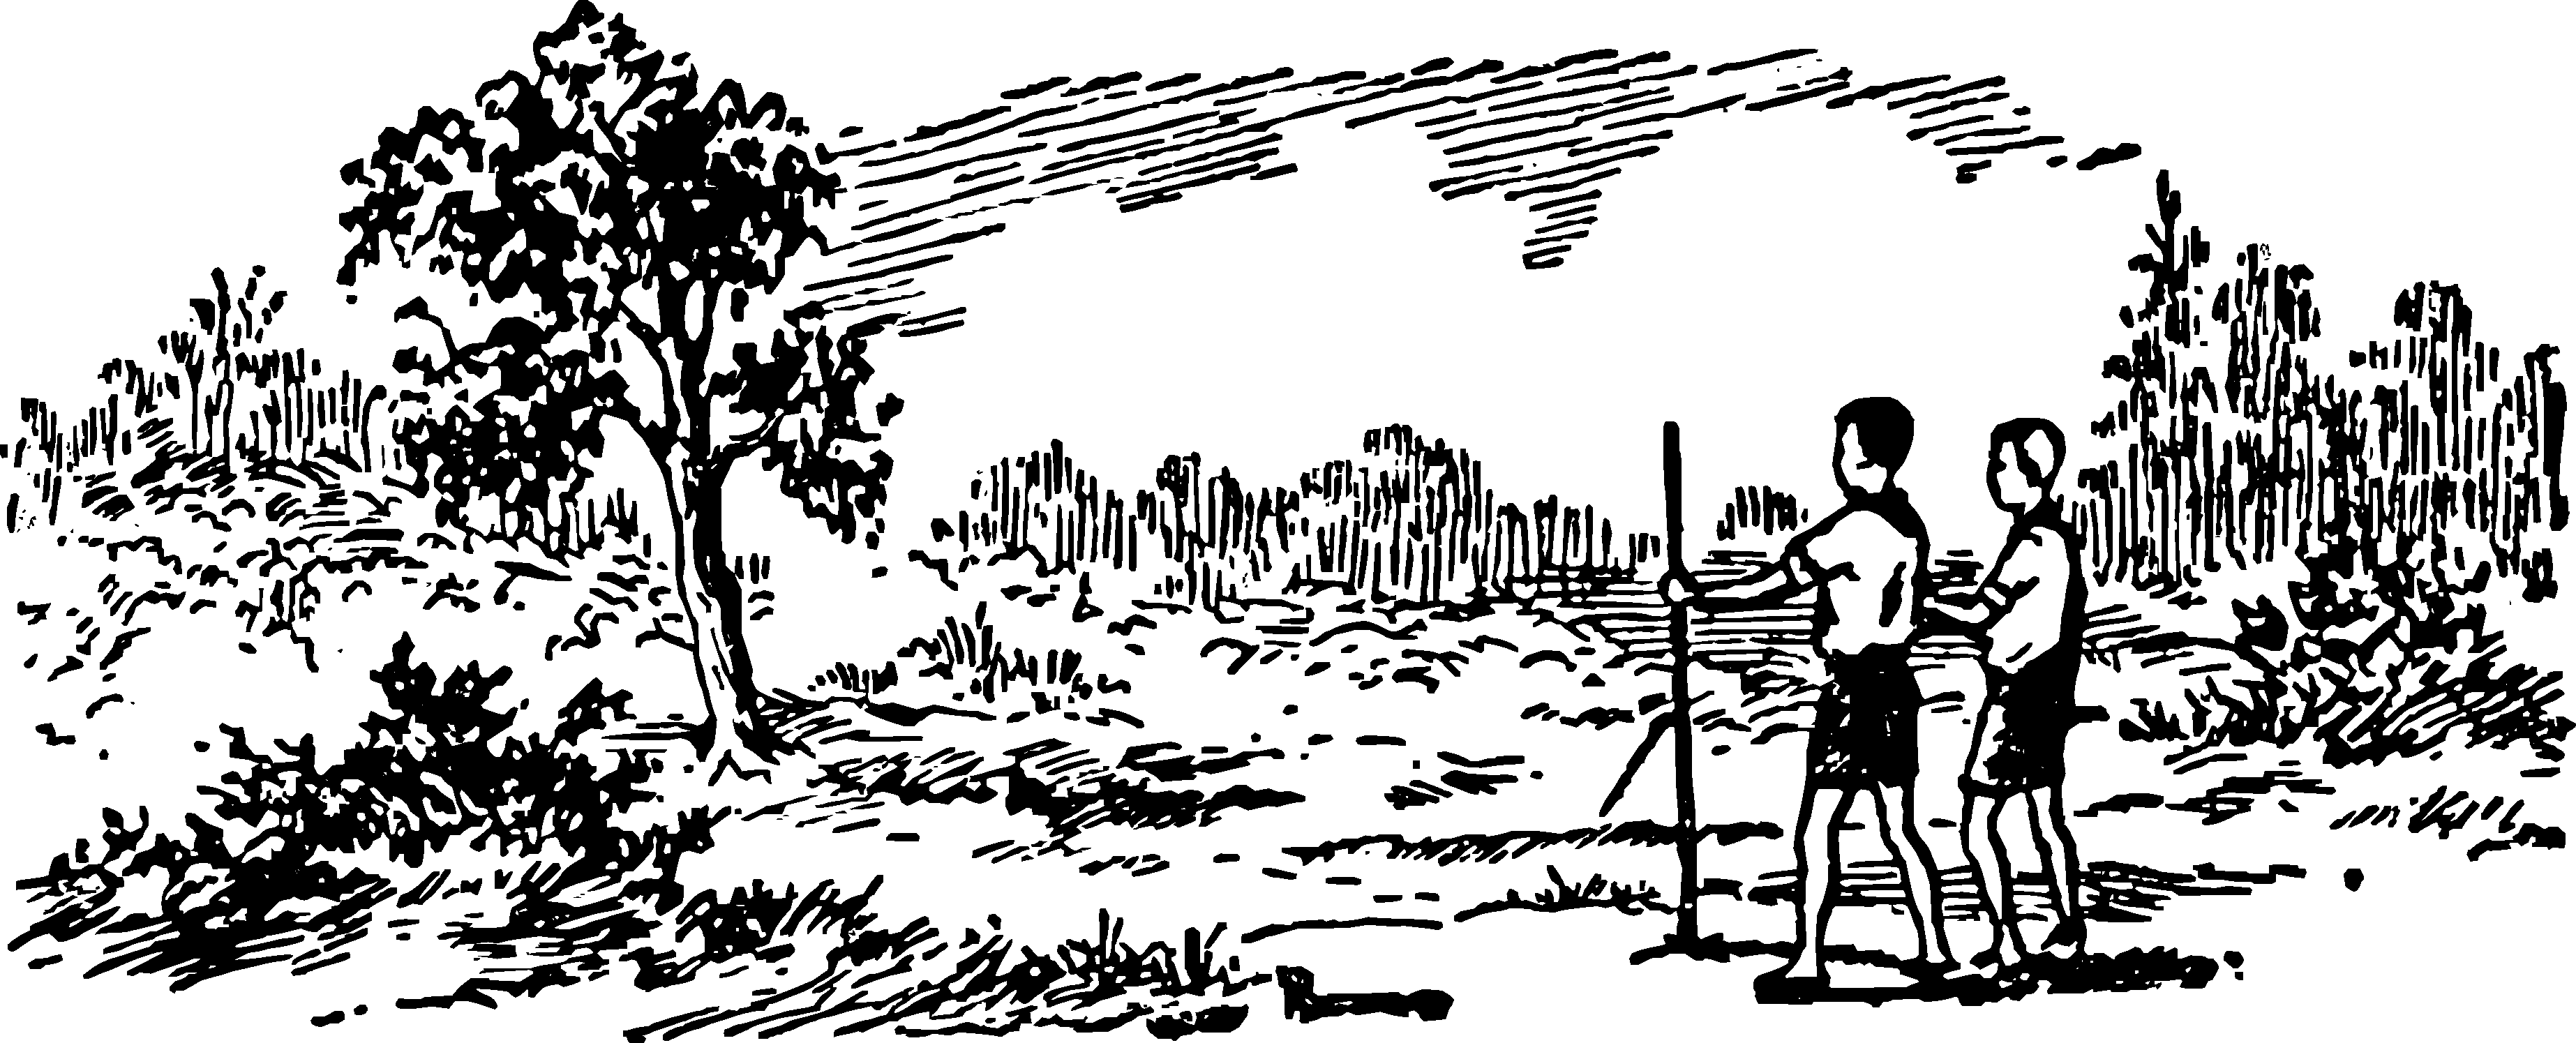
\includegraphics[width=1.2\textwidth]{figures/ch-01/fig-ch-01-head.pdf}};
%\end{scope}
%\end{tikzpicture}

\section{By the length of the shadow}
\label{sec-1.1}

I remember now the amazement with which I looked for the first time, he looked at a gray-haired forester, who, standing near a huge pine tree, measured its height with a small pocket device. When he aimed his square board at the top of the tree, I expected that the old man would now start climbing there with a measuring chain. Instead, he put the device back in his pocket and announced that the measurement was over. I thought it hadn't started yet \ldots{}

I was very young then, and this way of measuring, when a person determines the height of a tree without cutting it down and climbing to the top, was in my eyes something like a small miracle. It was only later, when I was initiated into the rudiments of geometry, that I realised how simple such miracles are performed. There are many different ways to make such measurements using very simple instruments and even without any devices.

The easiest and most ancient way is, without a doubt, the one by which the Greek sage Thales determined the height of the pyramid in Egypt sixth century BC. He took advantage of the pyramid's `shadow'. The priests and the pharaoh, gathered at the foot of the highest pyramid, looked puzzled at the northern newcomer, who guessed the height of the huge structure from the shadow. Thales, says the legend, chose a day and an hour when the length of his own shadow was equal to his height; at this moment, the height of the pyramid should also be equal to the length of the shadow cast by it\sidenote{Of course, the length of the shadow had to be measured from the midpoint of the square base of the pyramid; Thales could directly measure the width of this base.}. This is perhaps the only case when a person benefits from his shadow \ldots{}

The task of the Greek sage now seems childishly simple to us, but let's not forget that we are looking at it from the height of a geometric building erected after Thales. He lived long before Euclid, the author of the wonderful book that taught geometry for two millennia after his death. The truths contained in it, which are now known to every schoolboy, were not yet discovered in the era of Thales. And in order to use the shadow to solve the problem of the height of the pyramid, it was necessary to already know some geometric properties of the triangle, namely the following two (of which Thales himself discovered the first):
\begin{enumerate}
\item that the angles at the base of an isosceles triangle are equal, and vice versa -- that the sides lying opposite the equal angles of the triangle are equal to each other;
\item that the sum of the angles of any triangle (or at least a rectangular one) is equal to two right angles.
\end{enumerate}

Only Thales, armed with this knowledge, had the right to conclude that when his own shadow is equal to his height, the sun's rays meet the flat ground at an angle of half a straight line, and therefore the top of the pyramid, the middle of its base and the end of its shadow should mark an isosceles triangle.

It would seem that this simple method is very convenient to use on a clear sunny day to measure lonely trees whose shadow does not merge with the shadow of neighbouring ones. But in our latitudes it is not as easy as in Egypt to waylay the right moment for this: The sun is low above the horizon, and the shadows are equal to the height of the objects casting them only in the afternoon hours of the summer months. Therefore, the Thales method in this form is not always applicable.

\begin{figure}[h!]
\centering
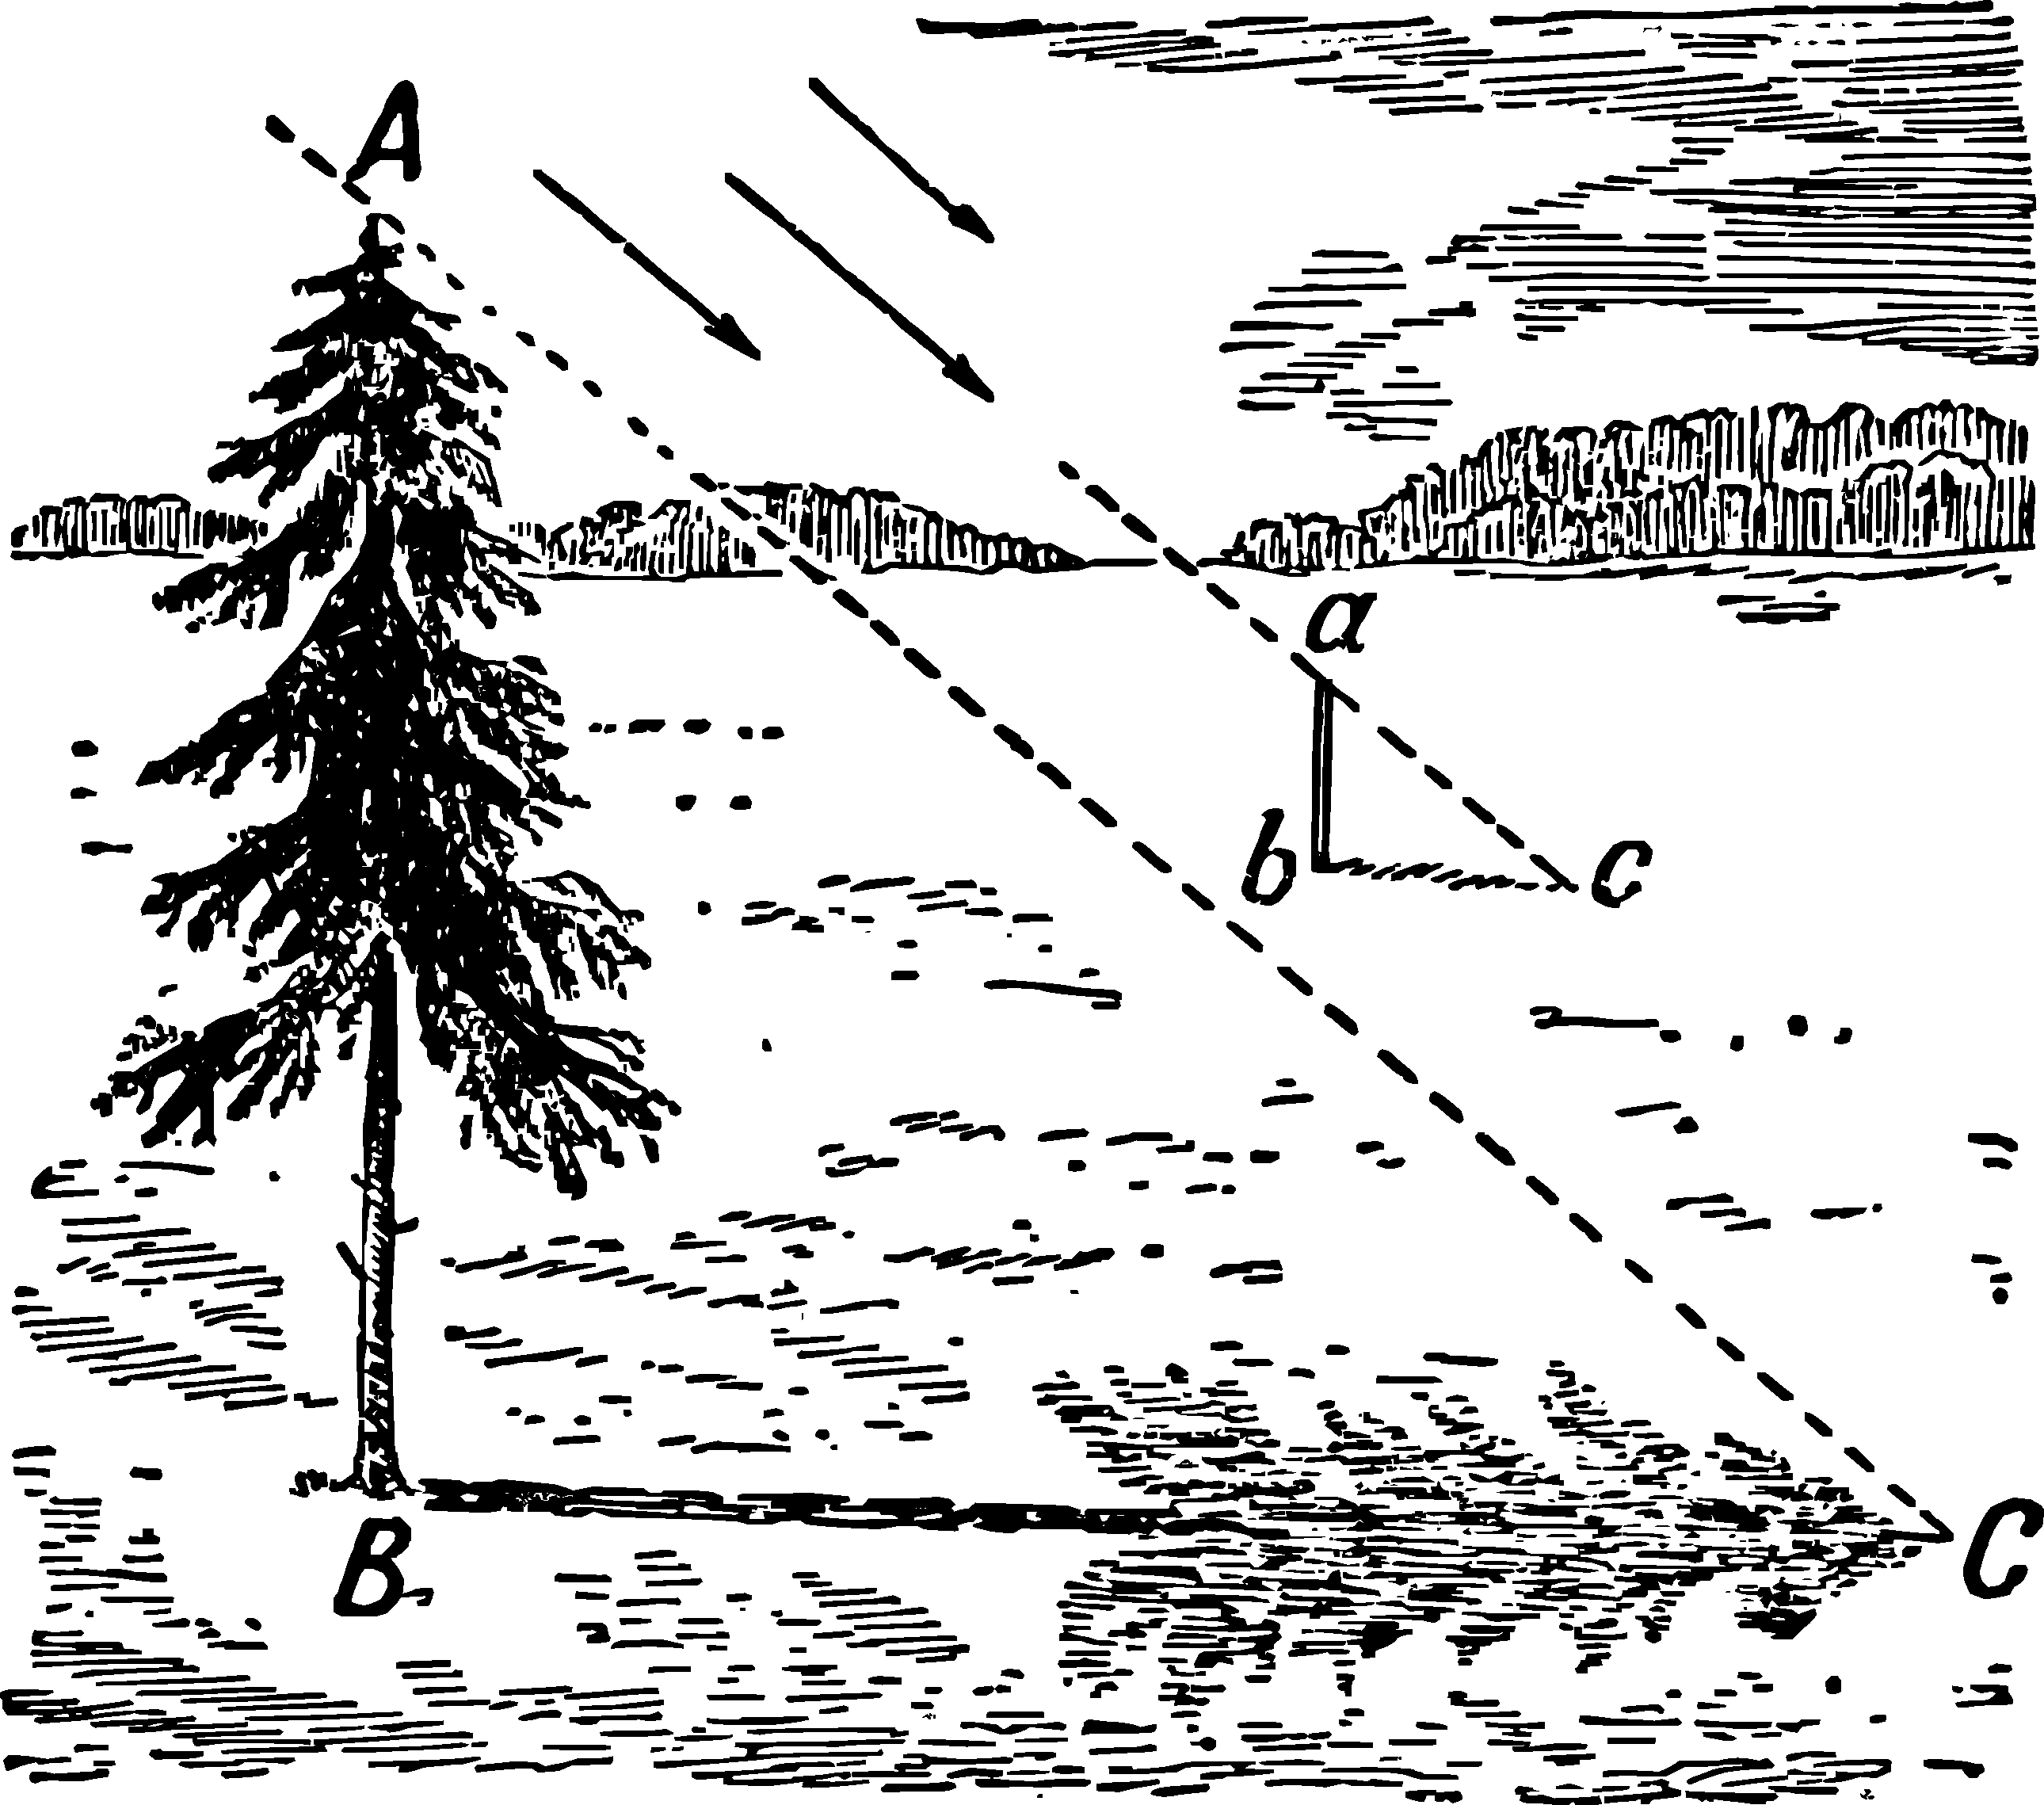
\includegraphics[width=0.9\textwidth]{figures/ch-01/fig-01-01.pdf}
\sidecaption{Measuring the height of a tree by shadow.\label{fig-01-01}}
\end{figure}
It is not difficult, however, to modify this method so that on a sunny day, any shadow can be used, regardless of its length. Additionally, measuring both your own shadow and the shadow of a pole, the desired height is calculated from the proportion (\figr{fig-01-01}):
\begin{equation*}%
AB:ab = BC:bc,
\end{equation*}
meaning the height of the tree is as many times greater than your own height (or the height of the pole) as the shadow of the tree is longer than your shadow (or the shadow of the pole). This naturally follows from the geometric similarity of triangles $ABC$ and $abc$ (based on two angles).

Some readers may object that such an elementary technique does not need a geometric justification at all: is it really unclear even without geometry that how many times is a tree taller, how many times is its shadow longer? However, the matter is not as simple as it seems. Try to apply this rule to shadows cast by the light of a street lamp or lamp -- it will not be justified. In \figr{fig-01-02} you can see that the columns $AB$ are about three times higher than the pedestal $ab$, and the shadow of the column is eight times larger than the shadow of the pedestal $(BC:bc)$. It is impossible to explain why the method is applicable in this case, but not in the other, without geometry.

\begin{figure}[h!]
\centering
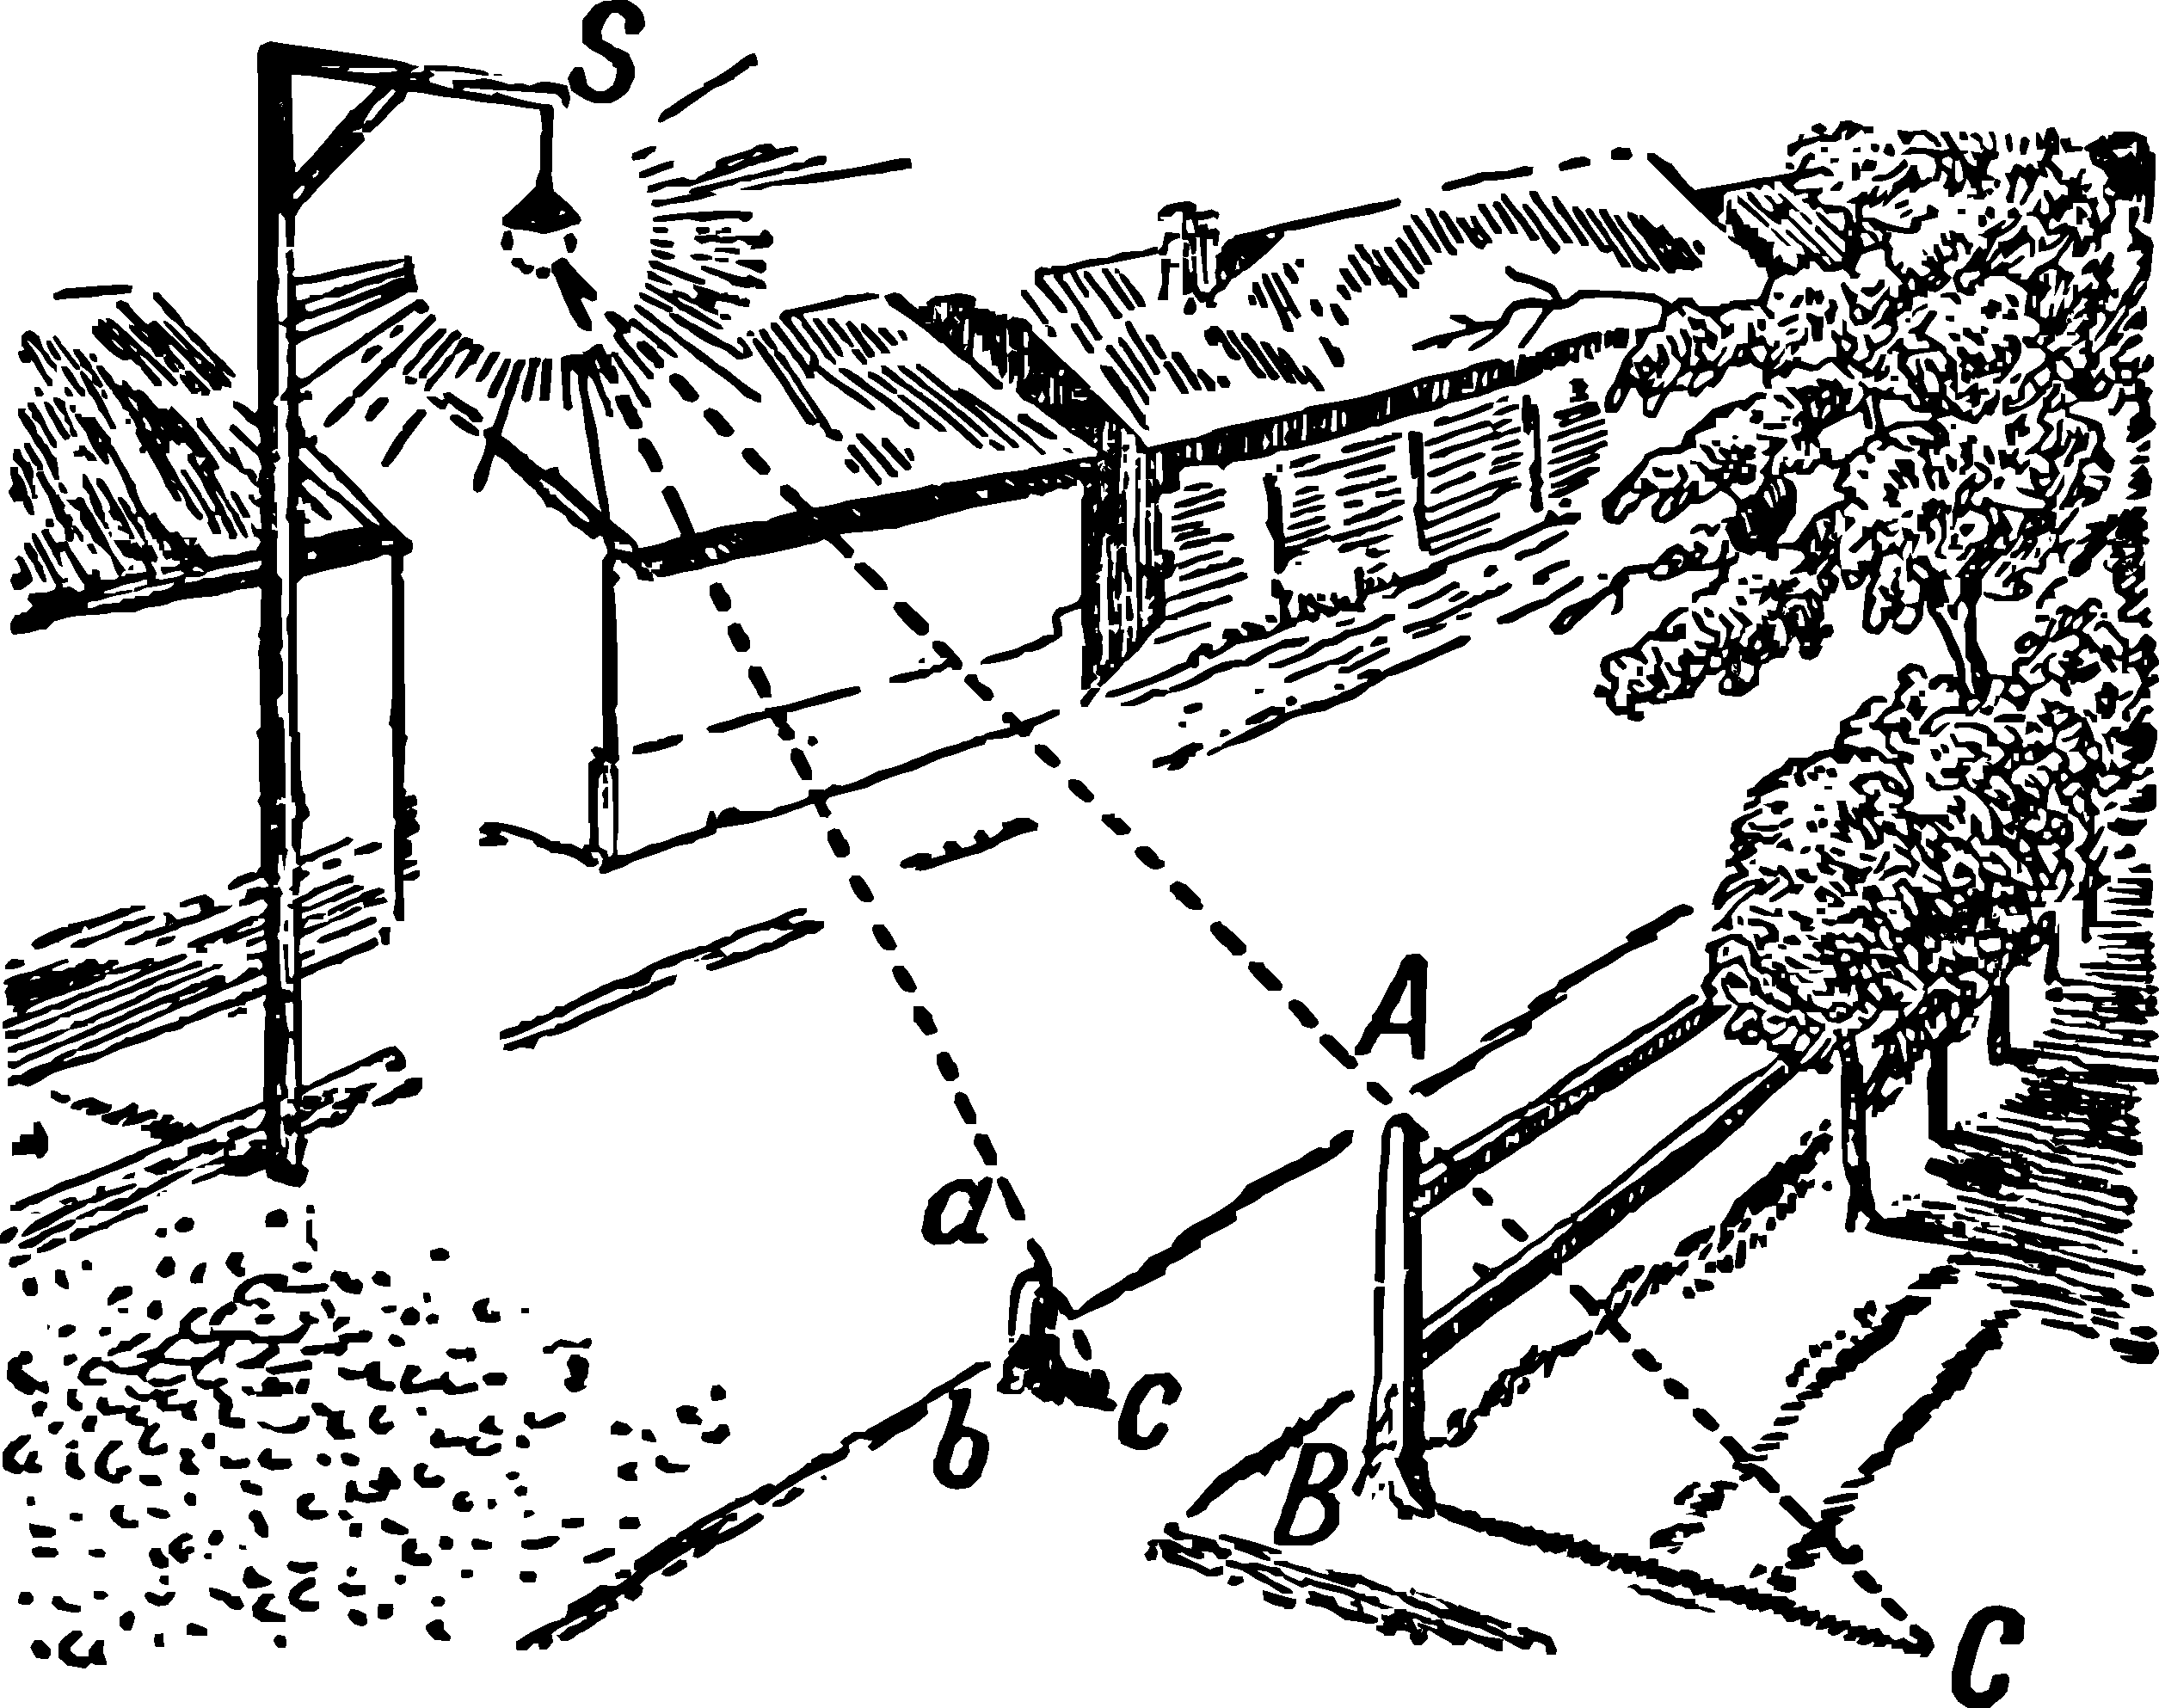
\includegraphics[width=0.9\textwidth]{figures/ch-01/fig-01-02.pdf}
\sidecaption[][0cm]{When such a measurement is impossible. (Is the method applicable for a shadow cast by a streetlamp?)\label{fig-01-02}}
\end{figure}


\ques Let's take a closer look at what the difference is. The essence of the matter boils down. to the fact that the sun's rays are parallel to each other, the rays of the lantern are not parallel. After that, we have the right to consider the rays of the Sun parallel, although they certainly intersect in the place from which they originate.


\ans The rays of the Sun falling on the Earth can be considered parallel because the angle between them is extremely small, almost imperceptible. A simple geometric calculation will convince you of this. Imagine two rays coming from some point of the Sun and falling on the Earth at a distance of, say, one kilo-meter from each other. So, if we put one leg of a compass at this point of the Sun, and with the other we described a circle with a radius equal to the distance from the Sun to the Earth (i.e., with a radius of \SI{150000000}{\kilo\meter}), then an arc of one kilometer in length would appear between our two radii rays. The total length of this gigantic circle would be equal to $2 \pi \times \SI{150000000}{\kilo\meter} = \SI{940000000}{\kilo\meter}$. One degree of it, of course, is 360 times less, i.e. about \SI{2600000}{\kilo\meter}; one arc minute is 60 times less than a degree, i.e. equal to \SI{43000}{\kilo\meter}, and one arc second is another 60 times less, i.e. \SI{720}{\kilo\meter}. But our arc is only \SI{1}{\kilo\meter} in length, so it corresponds to an angle of $1/720 \approx \ang{;;0.00138}$ seconds. This angle is elusive even for the most accurate astronomical instruments; therefore, in practise we can consider the rays of the Sun falling on the Earth as parallel lines.\sidenote{Another thing is the rays directed from some point of the Sun to the ends of the earth's diameter; the angle between them is large enough to measure (about \ang{;;17}); the definition of this angle gave astronomers one of the means to establish how great the distance from the Earth to the Sun is.}

Trying to apply the method of shadows in practise, you will immediately be convinced, however, of its unreliability. Shadows are not delimited so clearly that measuring their length can be done quite accurately. Each shadow cast by the light of the Sun has an indistinctly outlined grey border of penumbra, which gives the border of the shadow uncertainty. This is because the Sun is not a point, but a large luminous body emitting rays from many points. \figr{fig-01-03} illustrates why, as a result of this, the shadow of tree $AB$ also has an additional component in the form of half-shadow $CD$, gradually fading away.

\begin{figure}[h!]
\centering
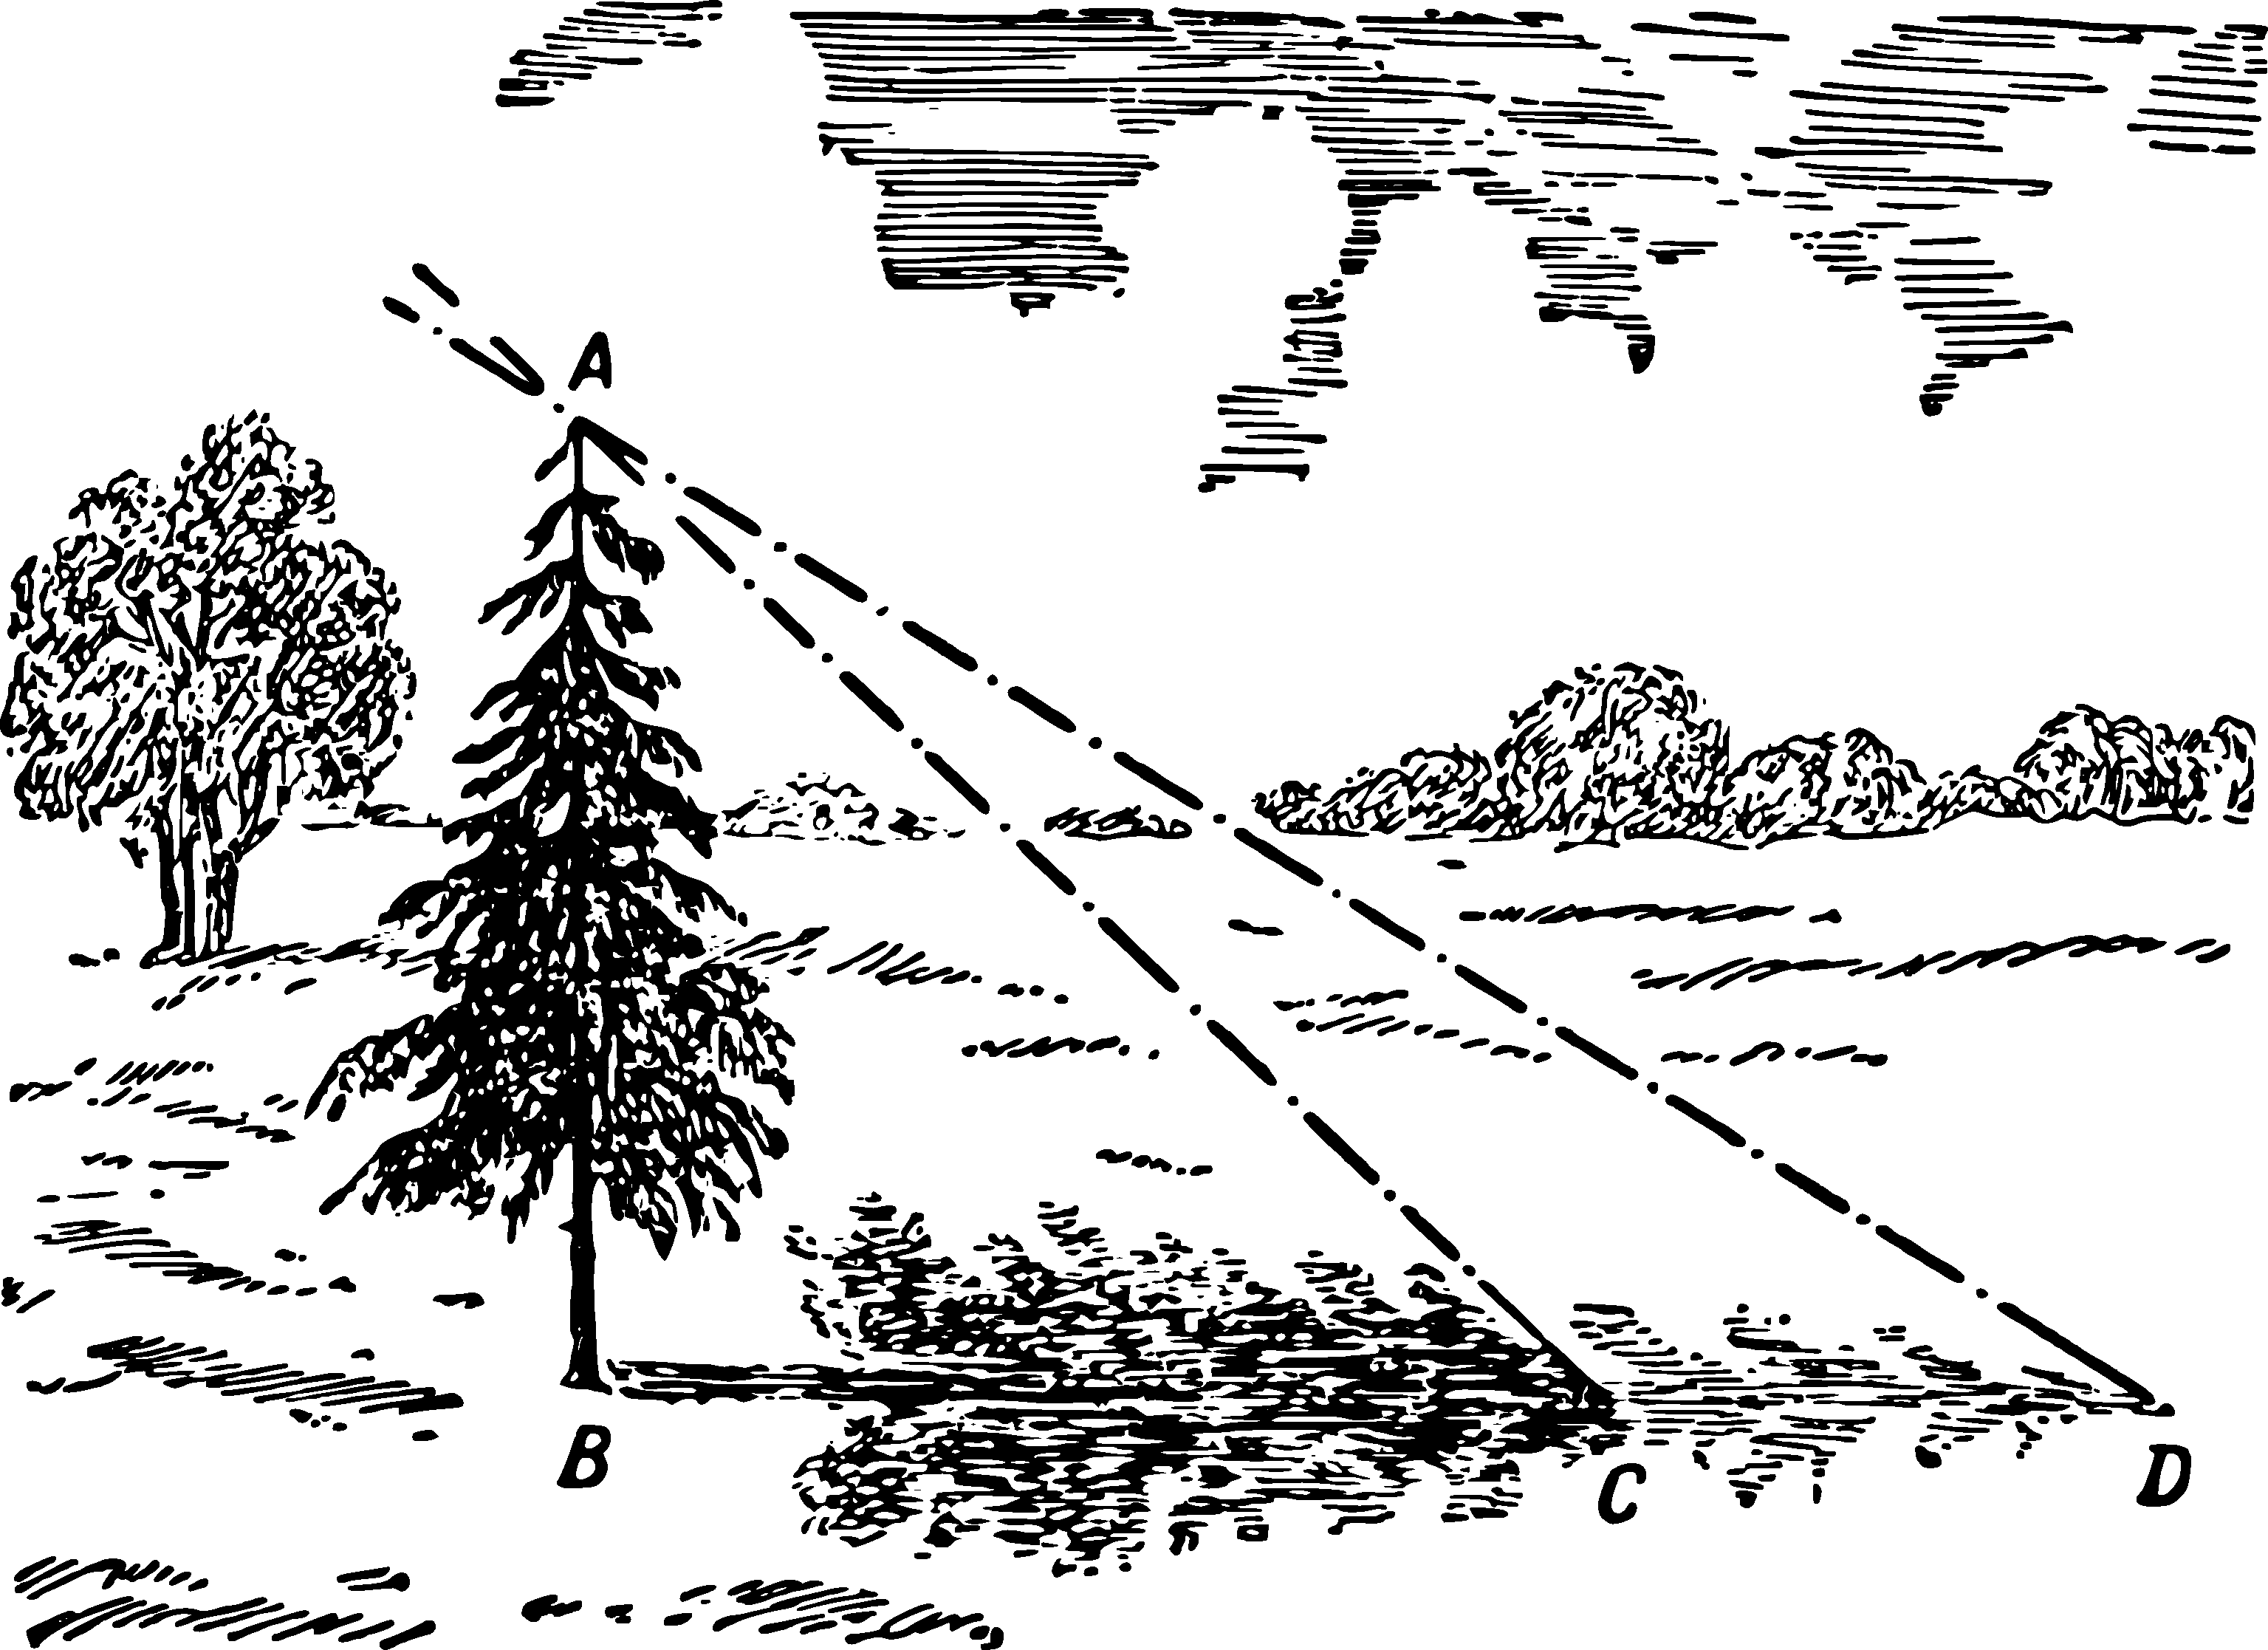
\includegraphics[width=0.9\textwidth]{figures/ch-01/fig-01-03.pdf}
\sidecaption{How penumbra is formed.\label{fig-01-03}}
\end{figure}


The angle of the $CAD$ between the extreme boundaries of the penumbra is equal to the angle at which we always see the solar disk, i.e. half a degree. The error resulting from the fact that both shadows are not measured quite accurately can reach 5\% or more when the Sun is not too low. This error is added to other unavoidable errors -- from uneven soil, etc. -- and makes the final result little reliable. In mountainous terrain, for example, this method is completely inapplicable.

\clearpage

\section{Two More Methods}
\label{sec-1.2}

It is entirely possible to measure height without relying on shadows. There are many methods; let's start with two simple ones.

Firstly, we can utilise the properties of an isosceles right triangle. For this purpose, we can make use of a very simple tool, which can be easily crafted from a piece of board and three pins. On a board of any shape, even a piece of bark with a flat side, mark three points to form the vertices of a right triangle -- and insert a pin at each point (see \figr{fig-01-04}). Suppose you don't have a drafting triangle to construct a right angle, nor a compass to mark equal sides. In that case, fold any piece of paper once, and then fold it again across the first fold so that both parts of the first fold coincide -- and you'll obtain a right angle. The same piece of paper can be used instead of a compass to measure equal distances.

\begin{figure}[h!]
\centering
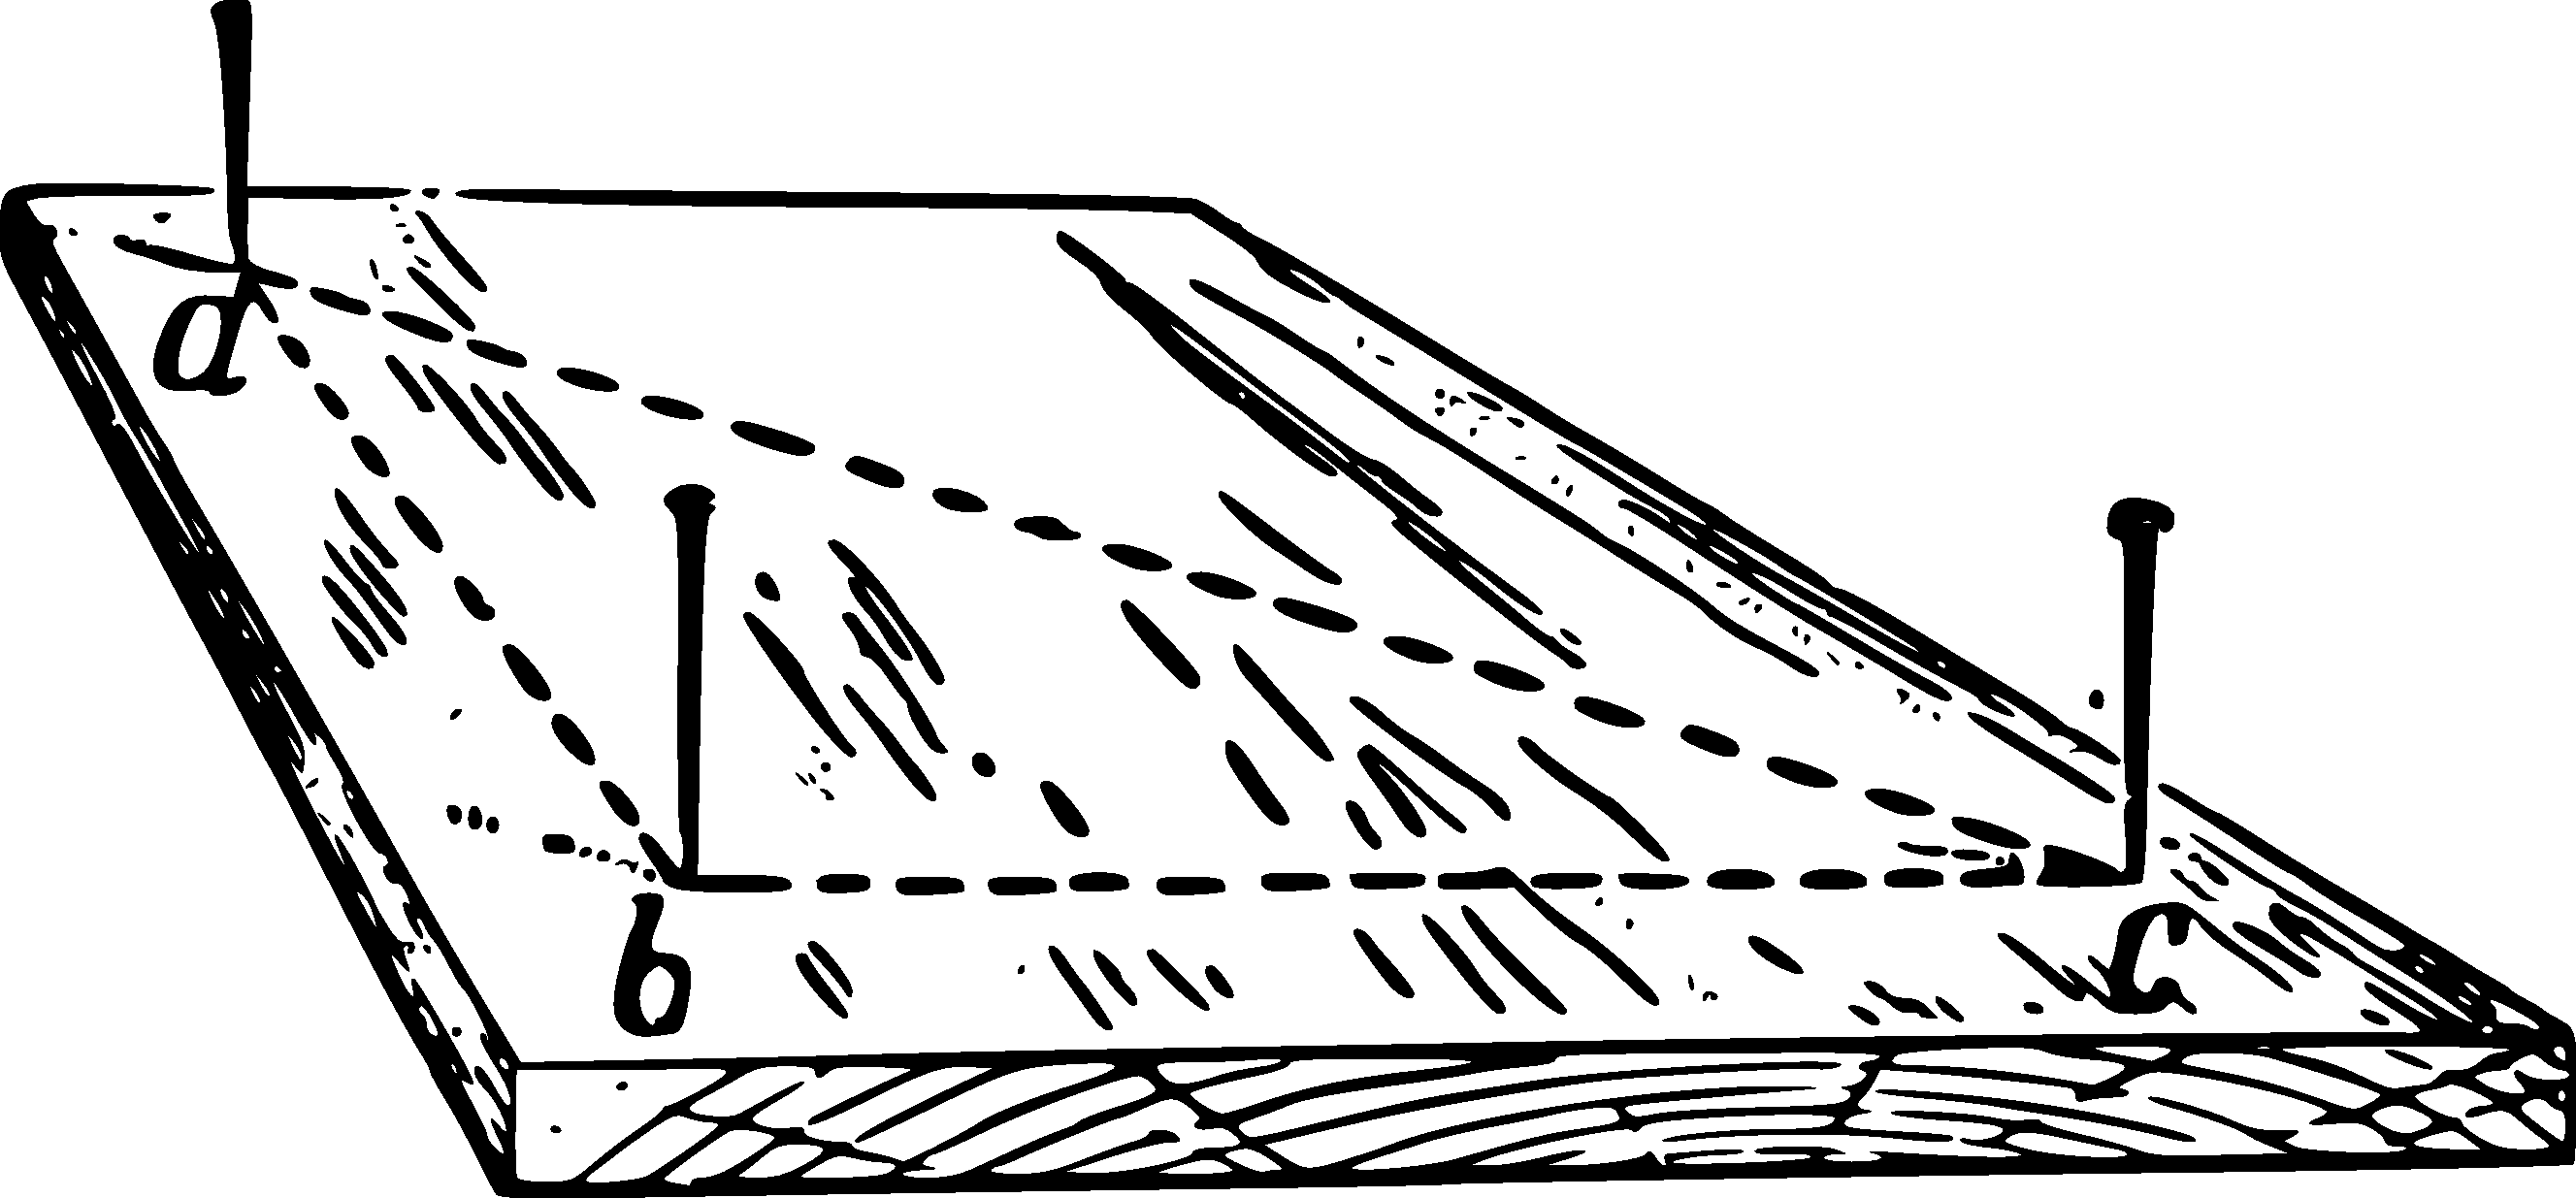
\includegraphics[width=0.6\textwidth]{figures/ch-01/fig-01-04.pdf}
\sidecaption{Pin height measuring device.\label{fig-01-04}}
\end{figure}


As you can see, the tool can be entirely crafted in a makeshift environment.

If you don't have a drafting triangle on hand to construct a right angle, nor a compass to mark equal sides, then simply fold any scrap of paper once, and then fold it again across the first fold so that both parts of the first fold coincide—and you'll obtain a right angle. The same piece of paper can be used instead of a compass to measure equal distances.

As you can see, the tool can be entirely crafted in a makeshift environment.

\begin{figure}[h!]
\centering
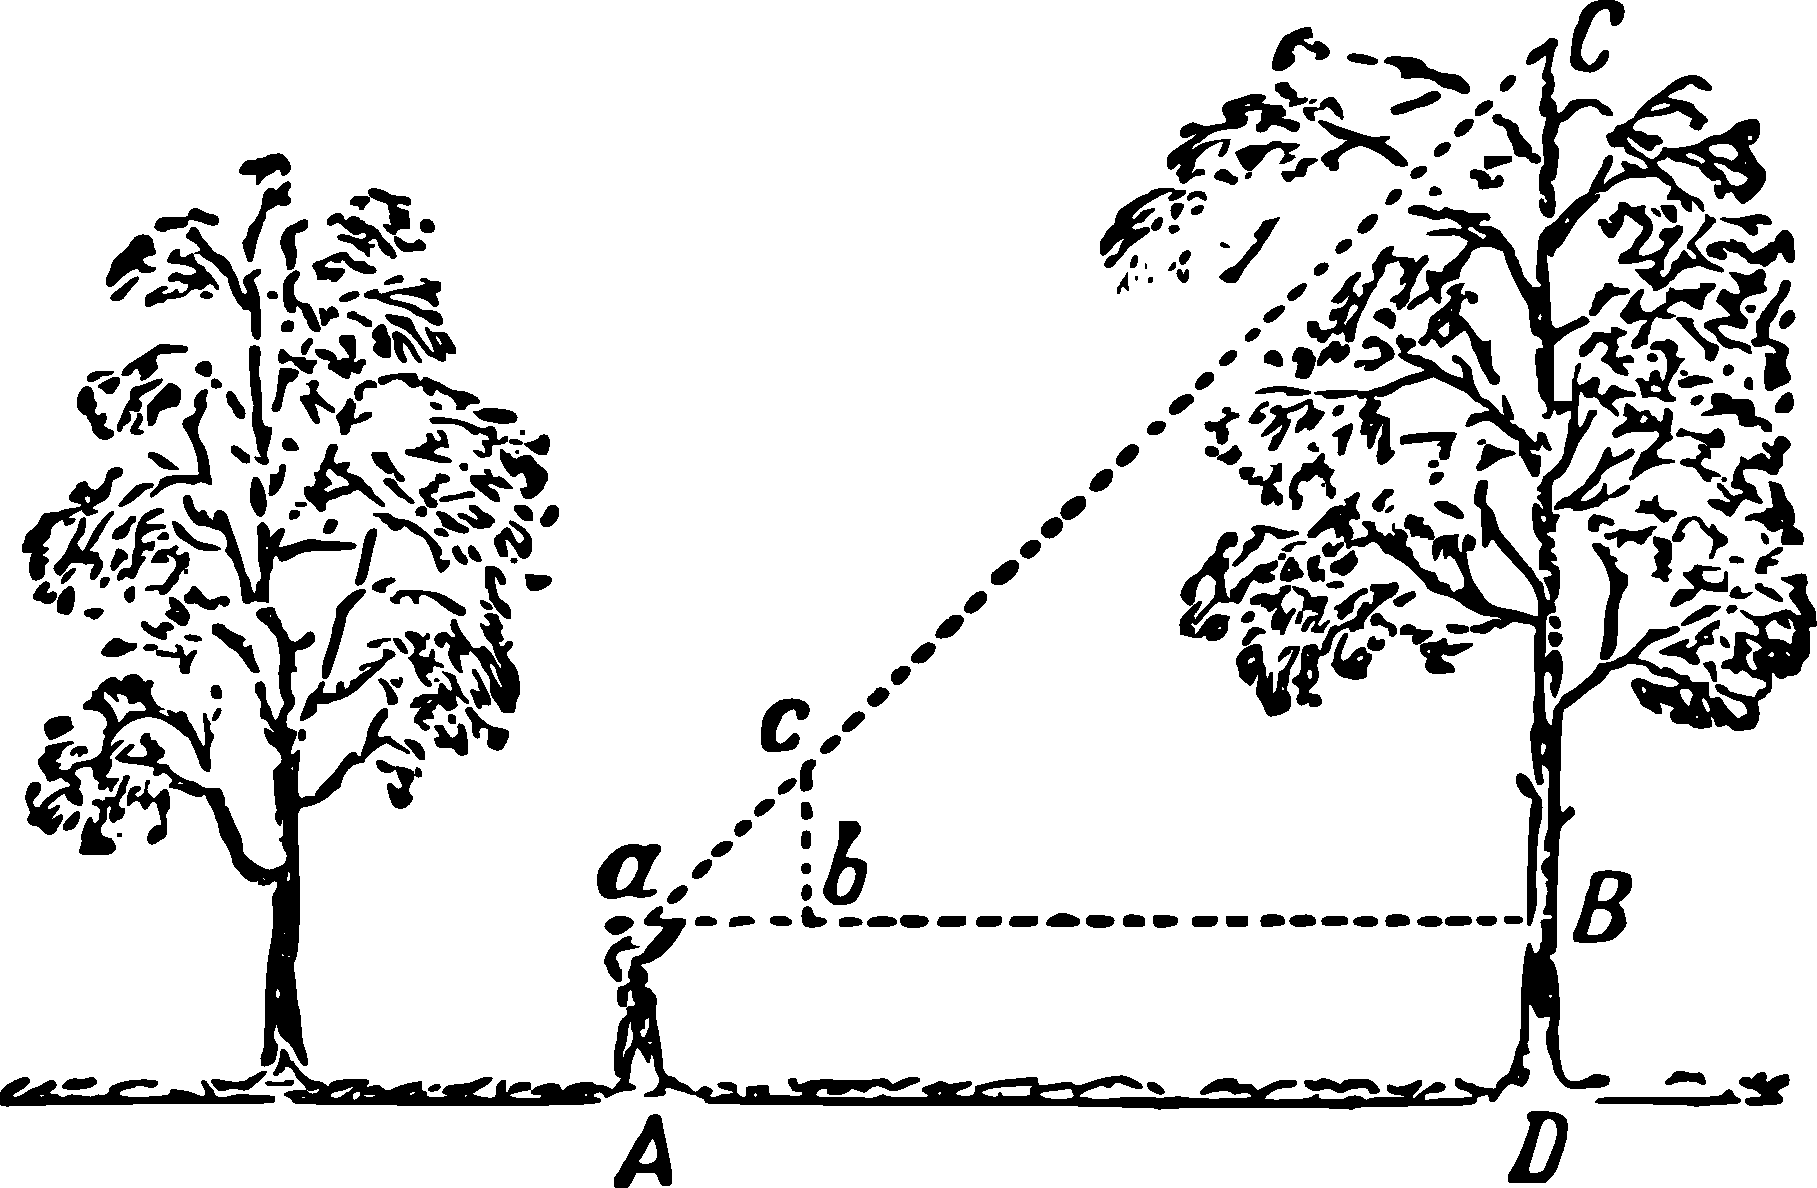
\includegraphics[width=0.9\textwidth]{figures/ch-01/fig-01-05.pdf}
\sidecaption{The scheme of application of the pin device.\label{fig-01-05}}
\end{figure}

Handling it is no more difficult than crafting it. Stepping away from the tree being measured, hold the tool so that one of the legs of the triangle is perpendicular. You can use a string or a weight tied to the top pin. Approaching or moving away from the tree, you will always find a spot $A$ (see \figr{fig-01-05}), from which, looking at pins $a$ and $c$, you will see that they cover the top $C$ of the tree: this means that the extension of the hypotenuse $ac$ passes through point $C$. Then, obviously, the distance $aB$ is equal to $CB$, since angle $a = \ang{45}$. 

Consequently, by measuring distance $aB$ (or, at another location, distance $AD$) and adding $BD$ to it, i.e., the elevation of point $a$ above the ground, you will obtain the desired height of the tree.

\begin{figure}[h!]
\centering
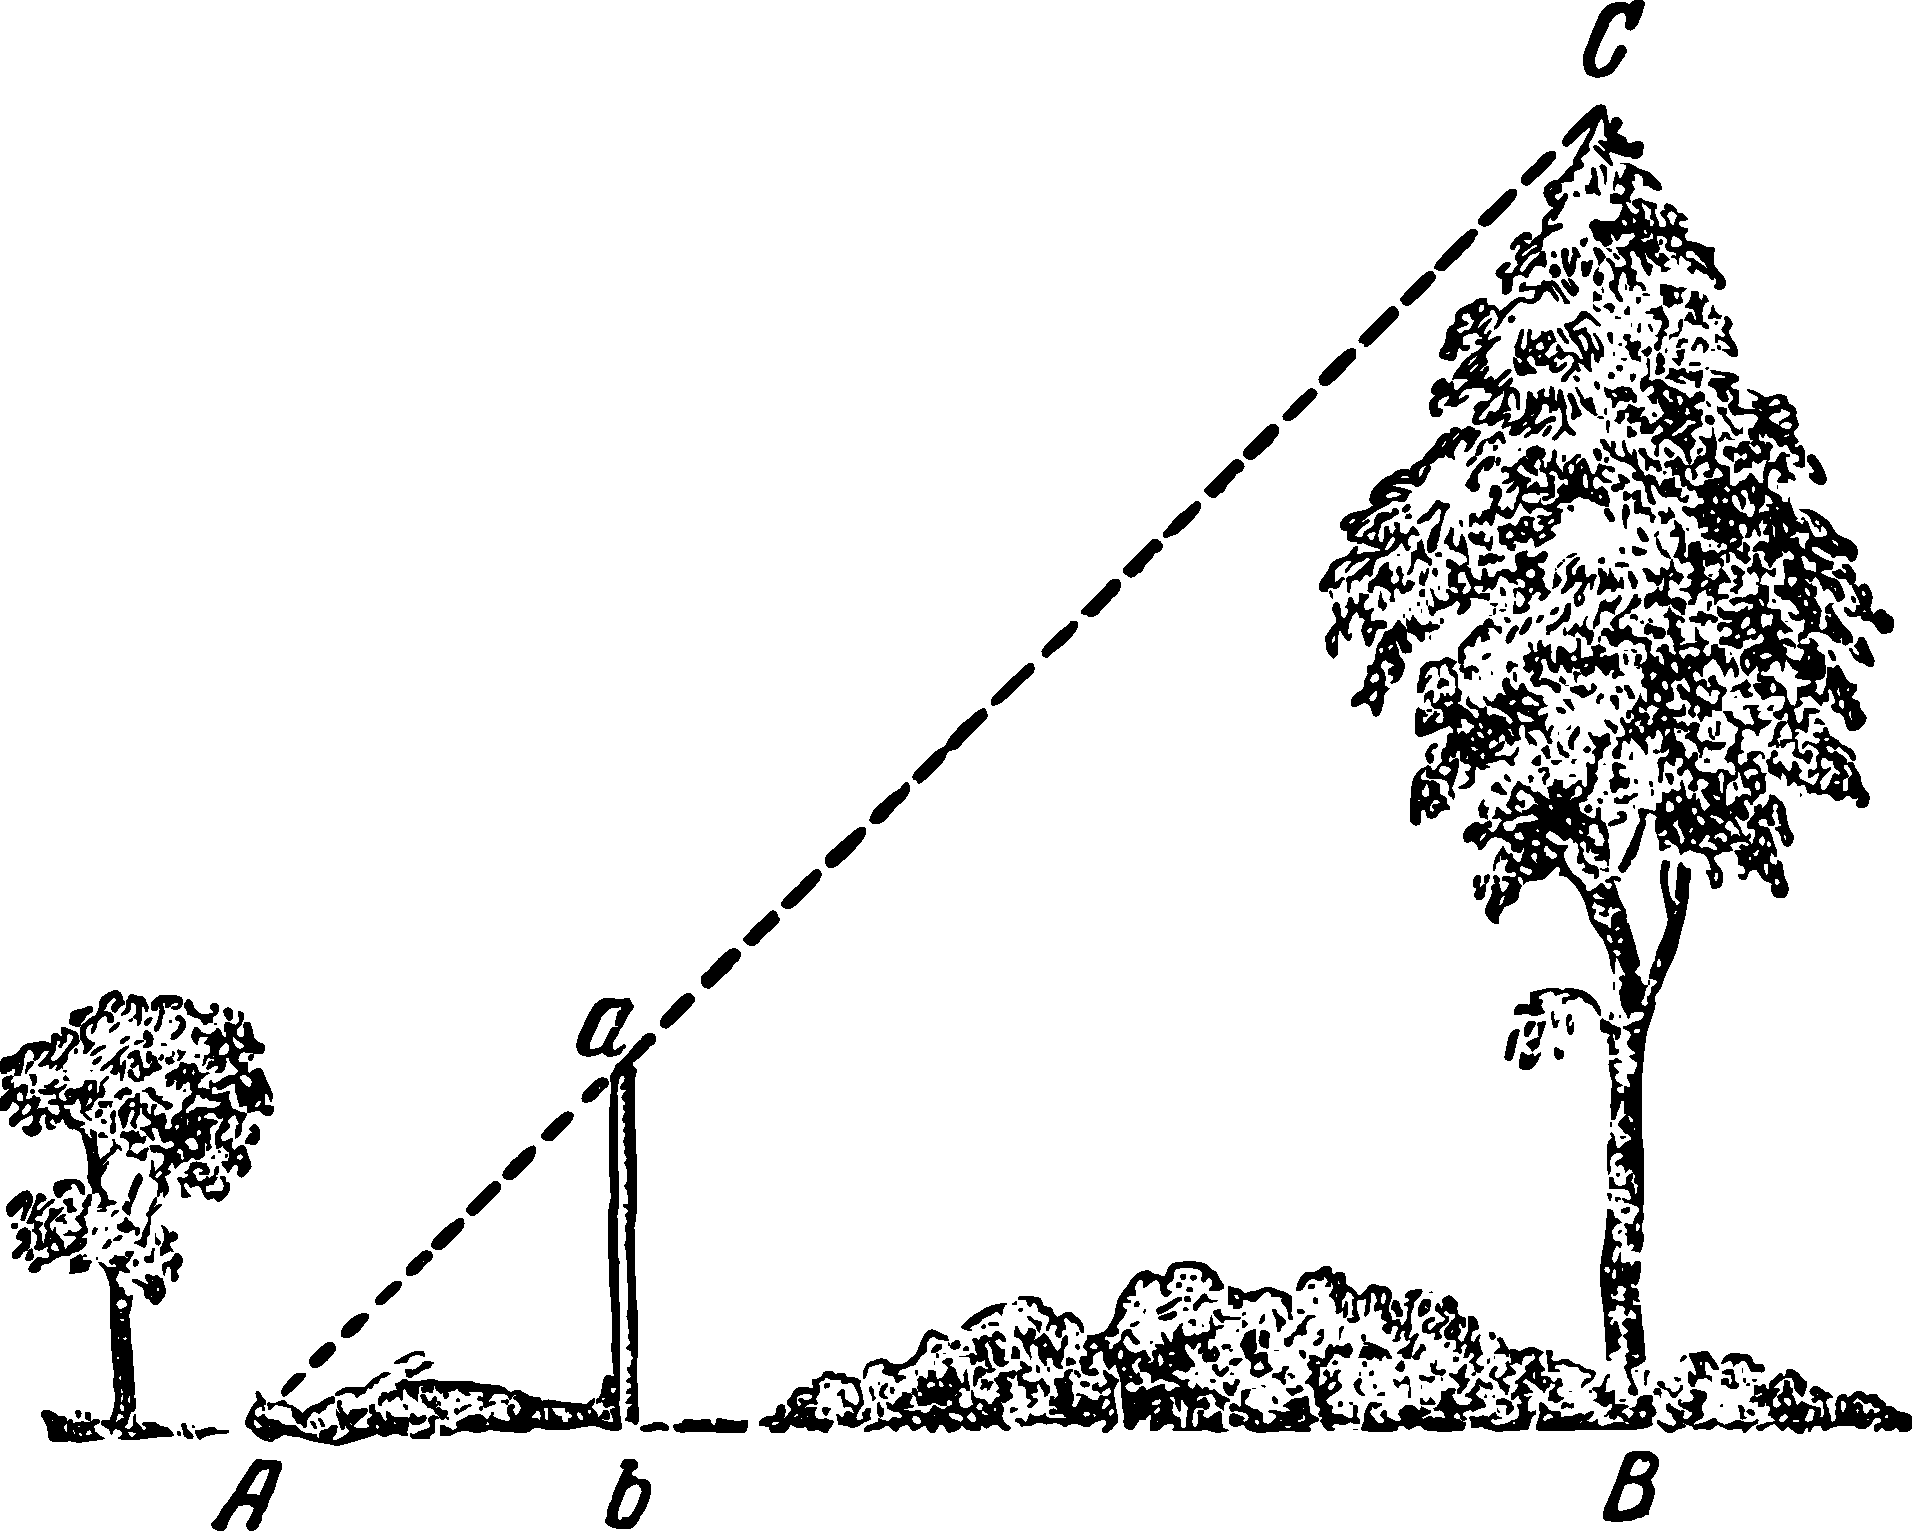
\includegraphics[width=0.9\textwidth]{figures/ch-01/fig-01-06.pdf}
\sidecaption{Another way to determine the height.\label{fig-01-06}}
\end{figure}

Another method does not even require a pin device. Here you need a pole, which you will have to insert vertically into the ground so that the protruding part is exactly at your height. The location for the pole must be chosen so that, lying down as shown in \figr{fig-01-06}, you see the top of the tree in a straight line with the upper point of the pole. Since triangle $Aba$ is isosceles and right-angled, angle $A = \ang{45}$, and therefore $AB$ equals $BC$, i.e., the desired height of the tree.



\section{The Method of Jules Verne}
\label{sec-1.3}

The next, also quite simple, method for measuring tall objects is vividly described by Jules Verne in his famous novel \emph{The Mysterious Island.}

``Today we need to measure the height of the Far View platform,'' said the engineer.

``Will you need a tool for that?'' asked Herbert.

``No, we won't. We'll proceed somewhat differently, resorting to a somewhat simpler and more accurate method.''

The young man, eager to learn as much as possible, followed the engineer, who descended from the granite wall to the rocky shore.

Taking a straight pole, twelve feet long, the engineer measured it as precisely as possible, comparing it to his own height, which he knew well. Meanwhile, Herbert held a plumb bob given to him by the engineer: just a stone attached to the end of a rope.

Not reaching five hundred feet from the granite wall, which rose vertically, the engineer drove the pole two feet into the sand and firmly secured it, placing it vertically with the help of the plumb bob.

\begin{figure}[h!]
\centering
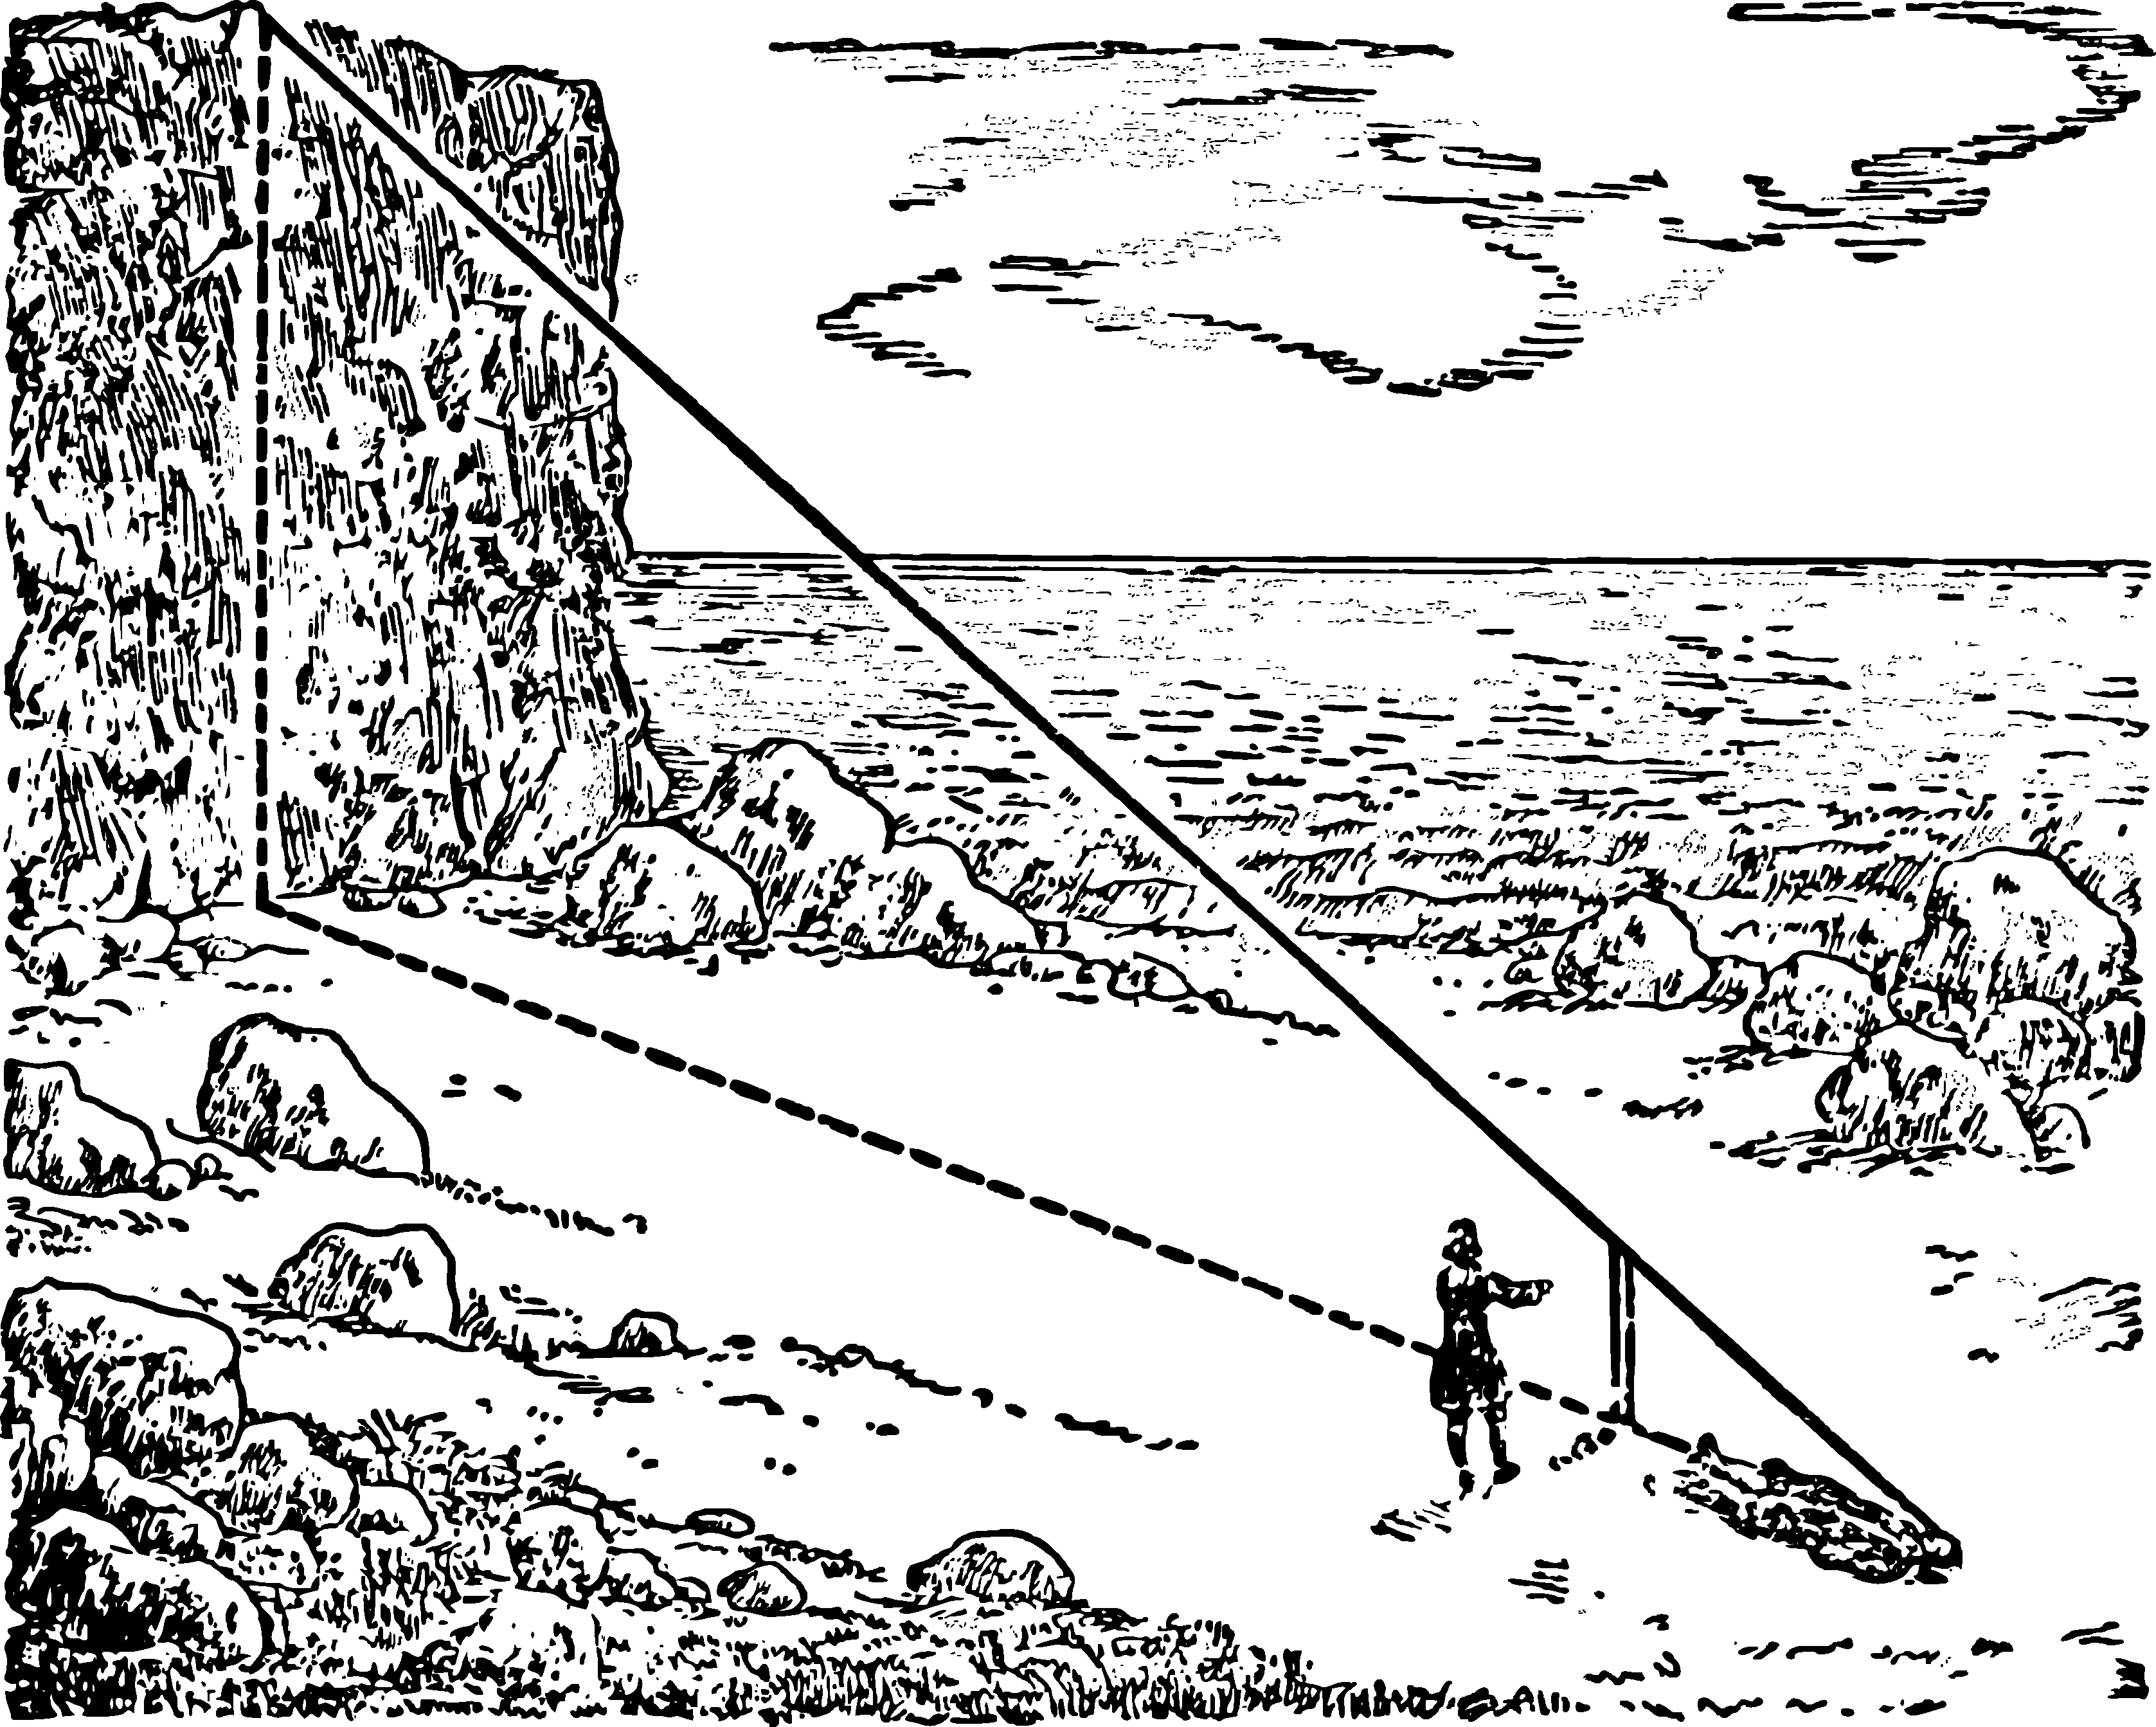
\includegraphics[width=0.9\textwidth]{figures/ch-01/fig-01-07.pdf}
\sidecaption{How the heroes of Jules Verne measured the height of the cliff.\label{fig-01-07}}
\end{figure}

Then he moved away from the pole to a distance where, lying on the sand, one could see both the end of the pole and the edge of the ridge in a straight line (see \figr{fig-01-07}). He carefully marked this point with a stake.

``Are you familiar with the basics of geometry?'' he asked Herbert as he rose from the ground.

``Yes.''

``Do you remember the properties of similar triangles?''

``Their corresponding sides are proportional.''

``Exactly. So now I'll construct two similar right triangles. In the smaller one, one leg will be the plumb-line pole, and the other will be the distance from the stake to the base of the pole; the hypotenuse will be my line of sight. In the other triangle, the legs will be: the granite wall, the height of which we want to determine, and the distance from the stake to the base of this wall; the hypotenuse will be my line of sight, coinciding with the direction of the hypotenuse of the first triangle.''

``Understood!'' exclaimed the youth. ``The distance from the stake to the pole is related to the distance from the stake to the base of the wall, as the height of the pole is to the height of the wall.''

``Yes. And consequently, if we measure the first two distances, then, knowing the height of the pole, we can calculate the fourth, unknown term of the proportion, i.e., the height of the wall. In this way, we can manage without directly measuring the height.''

Both horizontal distances were measured: the smaller one was 15 feet, the larger one was 500 feet.

At the end of the measurements, the engineer made the following record:
\begin{align*}%
15 : 500 & = 10 : x,\\
500 \times 10 & = 5000,\\
5000 : 15 & = 333.3.
\end{align*}
Thus, the height of the granite wall was 333 feet.


\section{How Sergeant Popov Acted}
\label{sec-1.4}

Some of the methods described for measuring height are inconvenient as they require lying on the ground. This inconvenience can, of course, be avoided.

Here's a story from one of the fronts of the Great Patriotic War. Lieutenant Ivanyuk's unit was ordered to build a bridge across a mountain river. On the opposite bank were entrenched fascists. To scout the location for the bridge, the lieutenant assigned a reconnaissance group led by Senior Sergeant Popov. In the nearest forest, they measured the diameter and height of the most typical trees and counted the number of trees that could be used for construction.

They measured the height of the trees using a pole (stick) as shown in \figr{fig-01-08}.

\begin{figure}[h!]
\centering
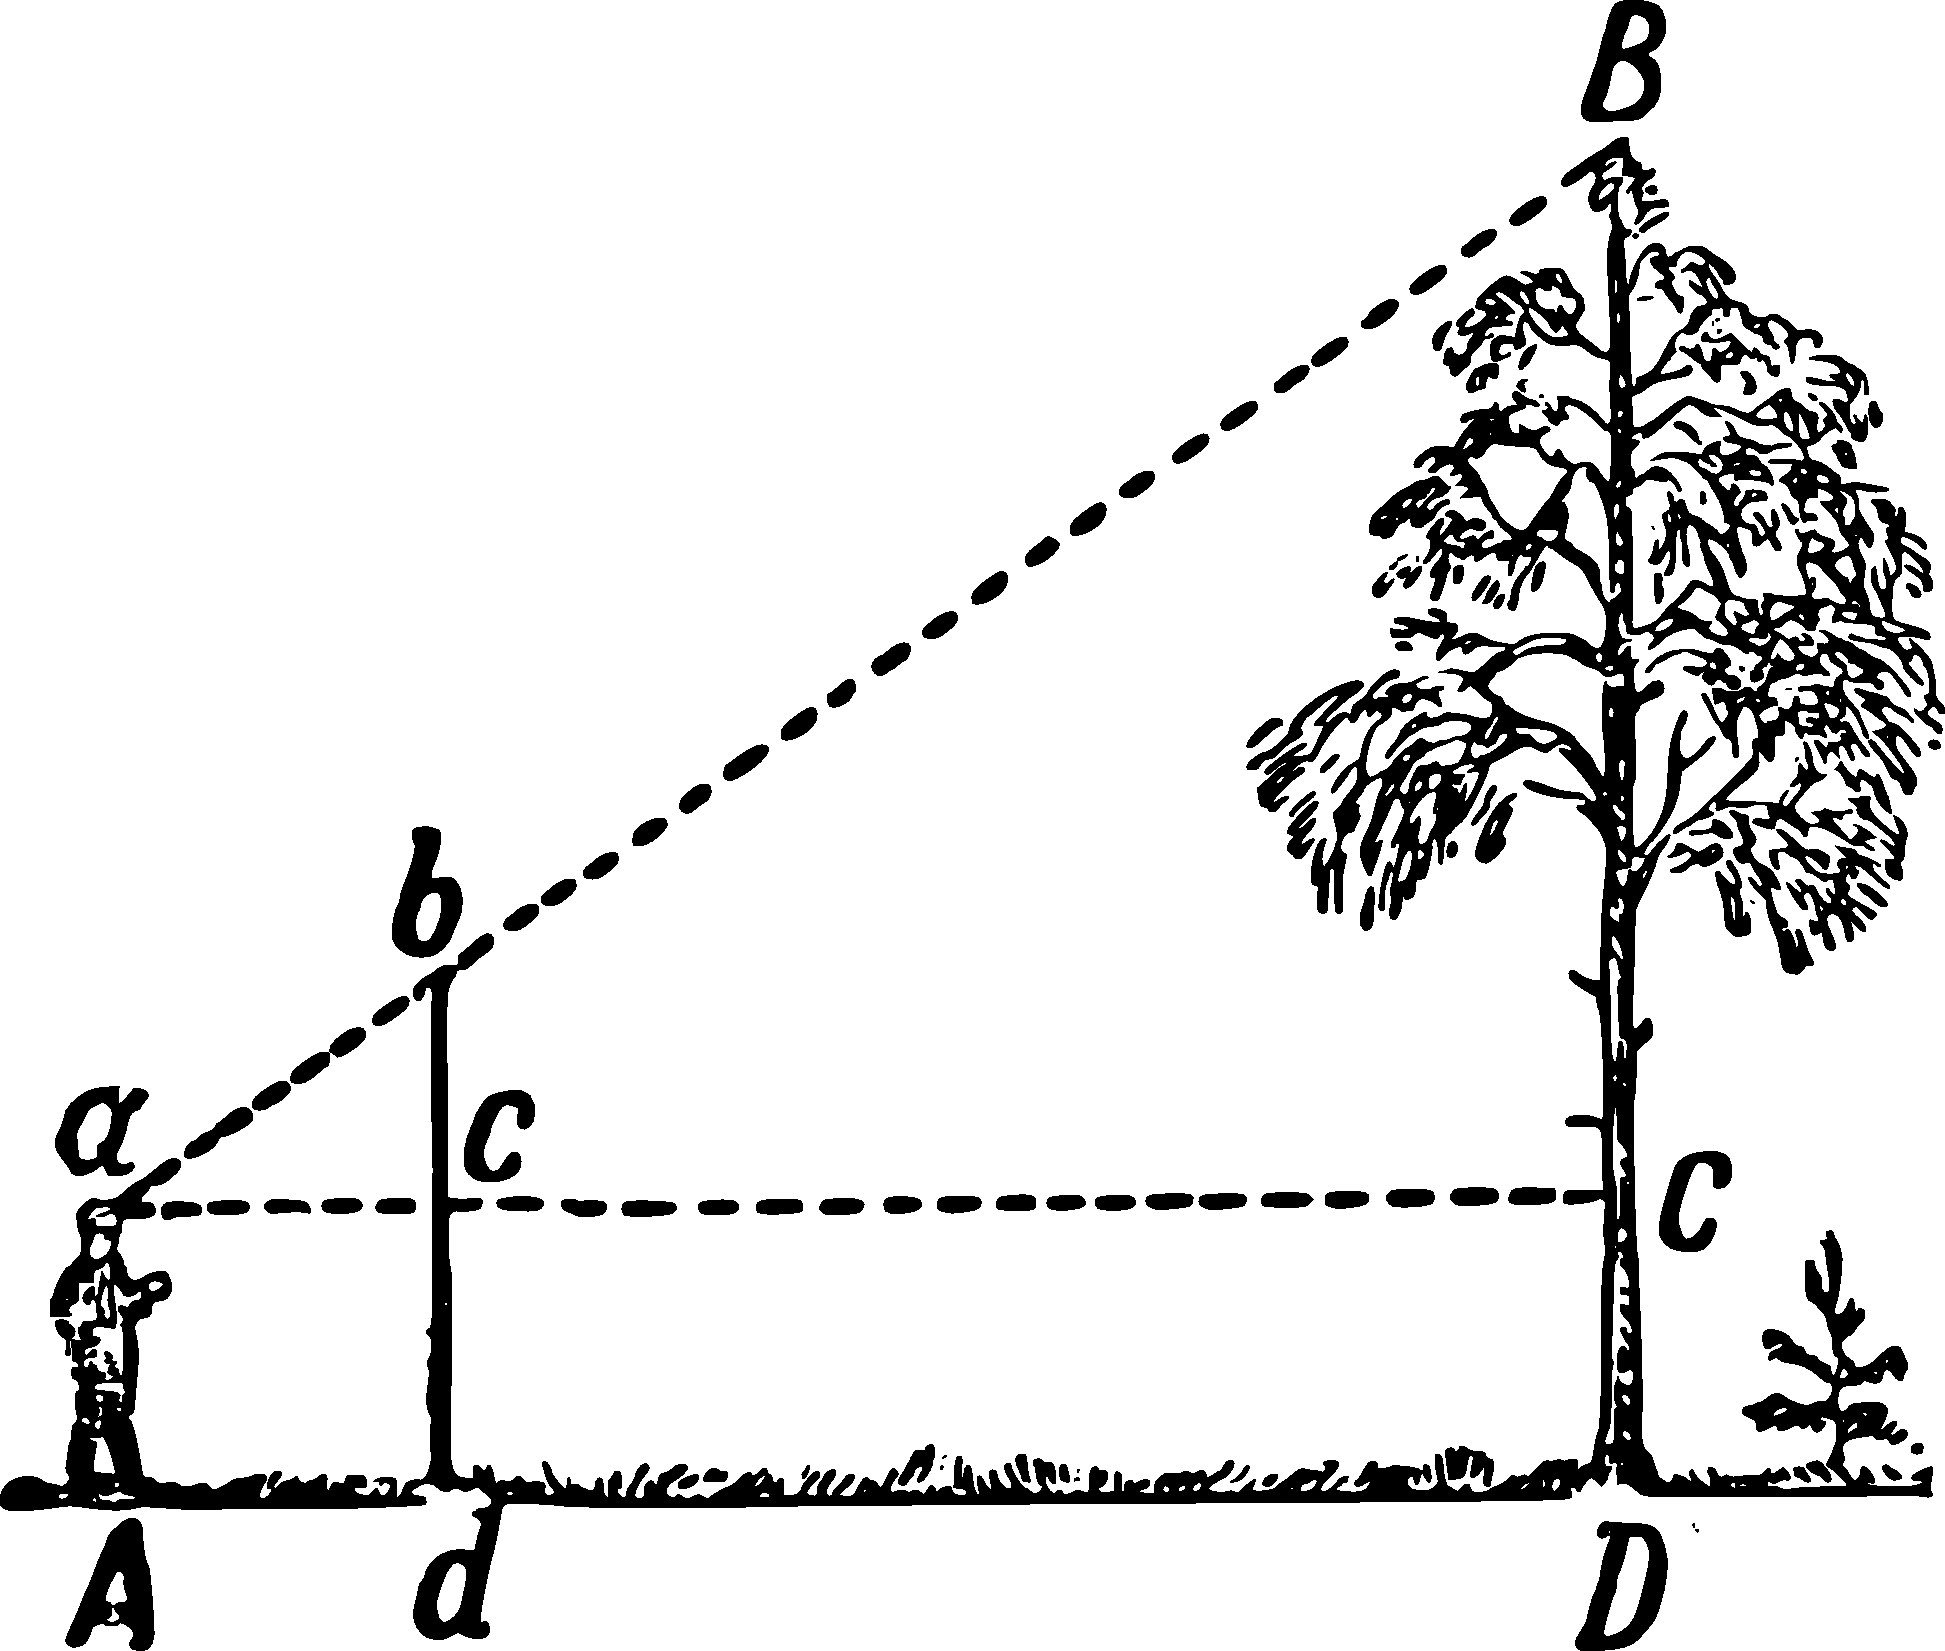
\includegraphics[width=0.6\textwidth]{figures/ch-01/fig-01-08.pdf}
\sidecaption{Measuring the height of the trees with a pole.\label{fig-01-08}}
\end{figure}

This method works as follows: Armed with a pole taller than your own height, drive it into the ground vertically at some distance from the tree being measured (see \figr{fig-01-08}). Step back from the pole along the line $dD$ until you reach point $A$, from where, looking at the top of the tree, you'll see the upper point $B$ of the pole aligned with it. Then, without changing the position of your head, look along the horizontal line $aC$, noting the point $C$ where your line of sight intersects the pole and the tree trunk. Ask your assistant to mark these points, and the observation is complete. Then, based on the similarity of triangles $abc$ and $aBC$, calculate $BC$ from the proportion 
\begin{equation*}%
\frac{BC}{bc} = \frac{aC}{ac},
\end{equation*}
and thus
\begin{equation*}%
BC = bc \cdot \frac{aC}{ac}
\end{equation*}
The distances $bc$, $aC$, and $ac$ can be easily measured directly. To obtain the actual height of the tree, add the distance $BC$ to the distance $CD$, which is also measured directly.

To determine the number of trees, the senior sergeant ordered the soldiers to measure the area of the forest. Then he counted the number of trees in a small area measuring 50 by 50 meters and multiplied accordingly.

Based on all the data collected by the scouts, the unit commander determined where and what kind of bridge needed to be built. The bridge was completed on time, and the combat mission was successfully accomplished!\sidenote{The episodes of the Great Patriotic War described here and further are narrated by A. Demidov in the journal \emph{Military Knowledge} No. 8, 1949, in the article \emph{River Reconnaissance.}\label{ref-21}}

\clearpage

\section{Using a Notebook}
\label{sec-1.5}

As a device for an approximate estimate of the inaccessible height, you can also use your pocket back book, if it is equipped with a pencil stuck in a cover or a loop with a book. It will help you to build in space those two similar triangles, from which the desired height is obtained. The book should be held near the eyes as shown in the simplified \figr{fig-01-09}. It should be in the vertical book so that, looking from the point $a$, you can see the top of the tree $B$ covered with the tip of the pencil $b$. Then, due to the similarity of the triangles $abc$ and $aBC$, the height of the $BC$ will be determined from the proportion
\begin{equation*}%
\frac{BC}{bc} = \frac{aC}{ac}.
\end{equation*}
The distances of $bc$, $ac$ and $aC$ are measured directly. To the resulting value of the $BC$, add the length of $CD$, which is, on level ground, the height of the eyes above the ground


\begin{figure}[h!]
\centering
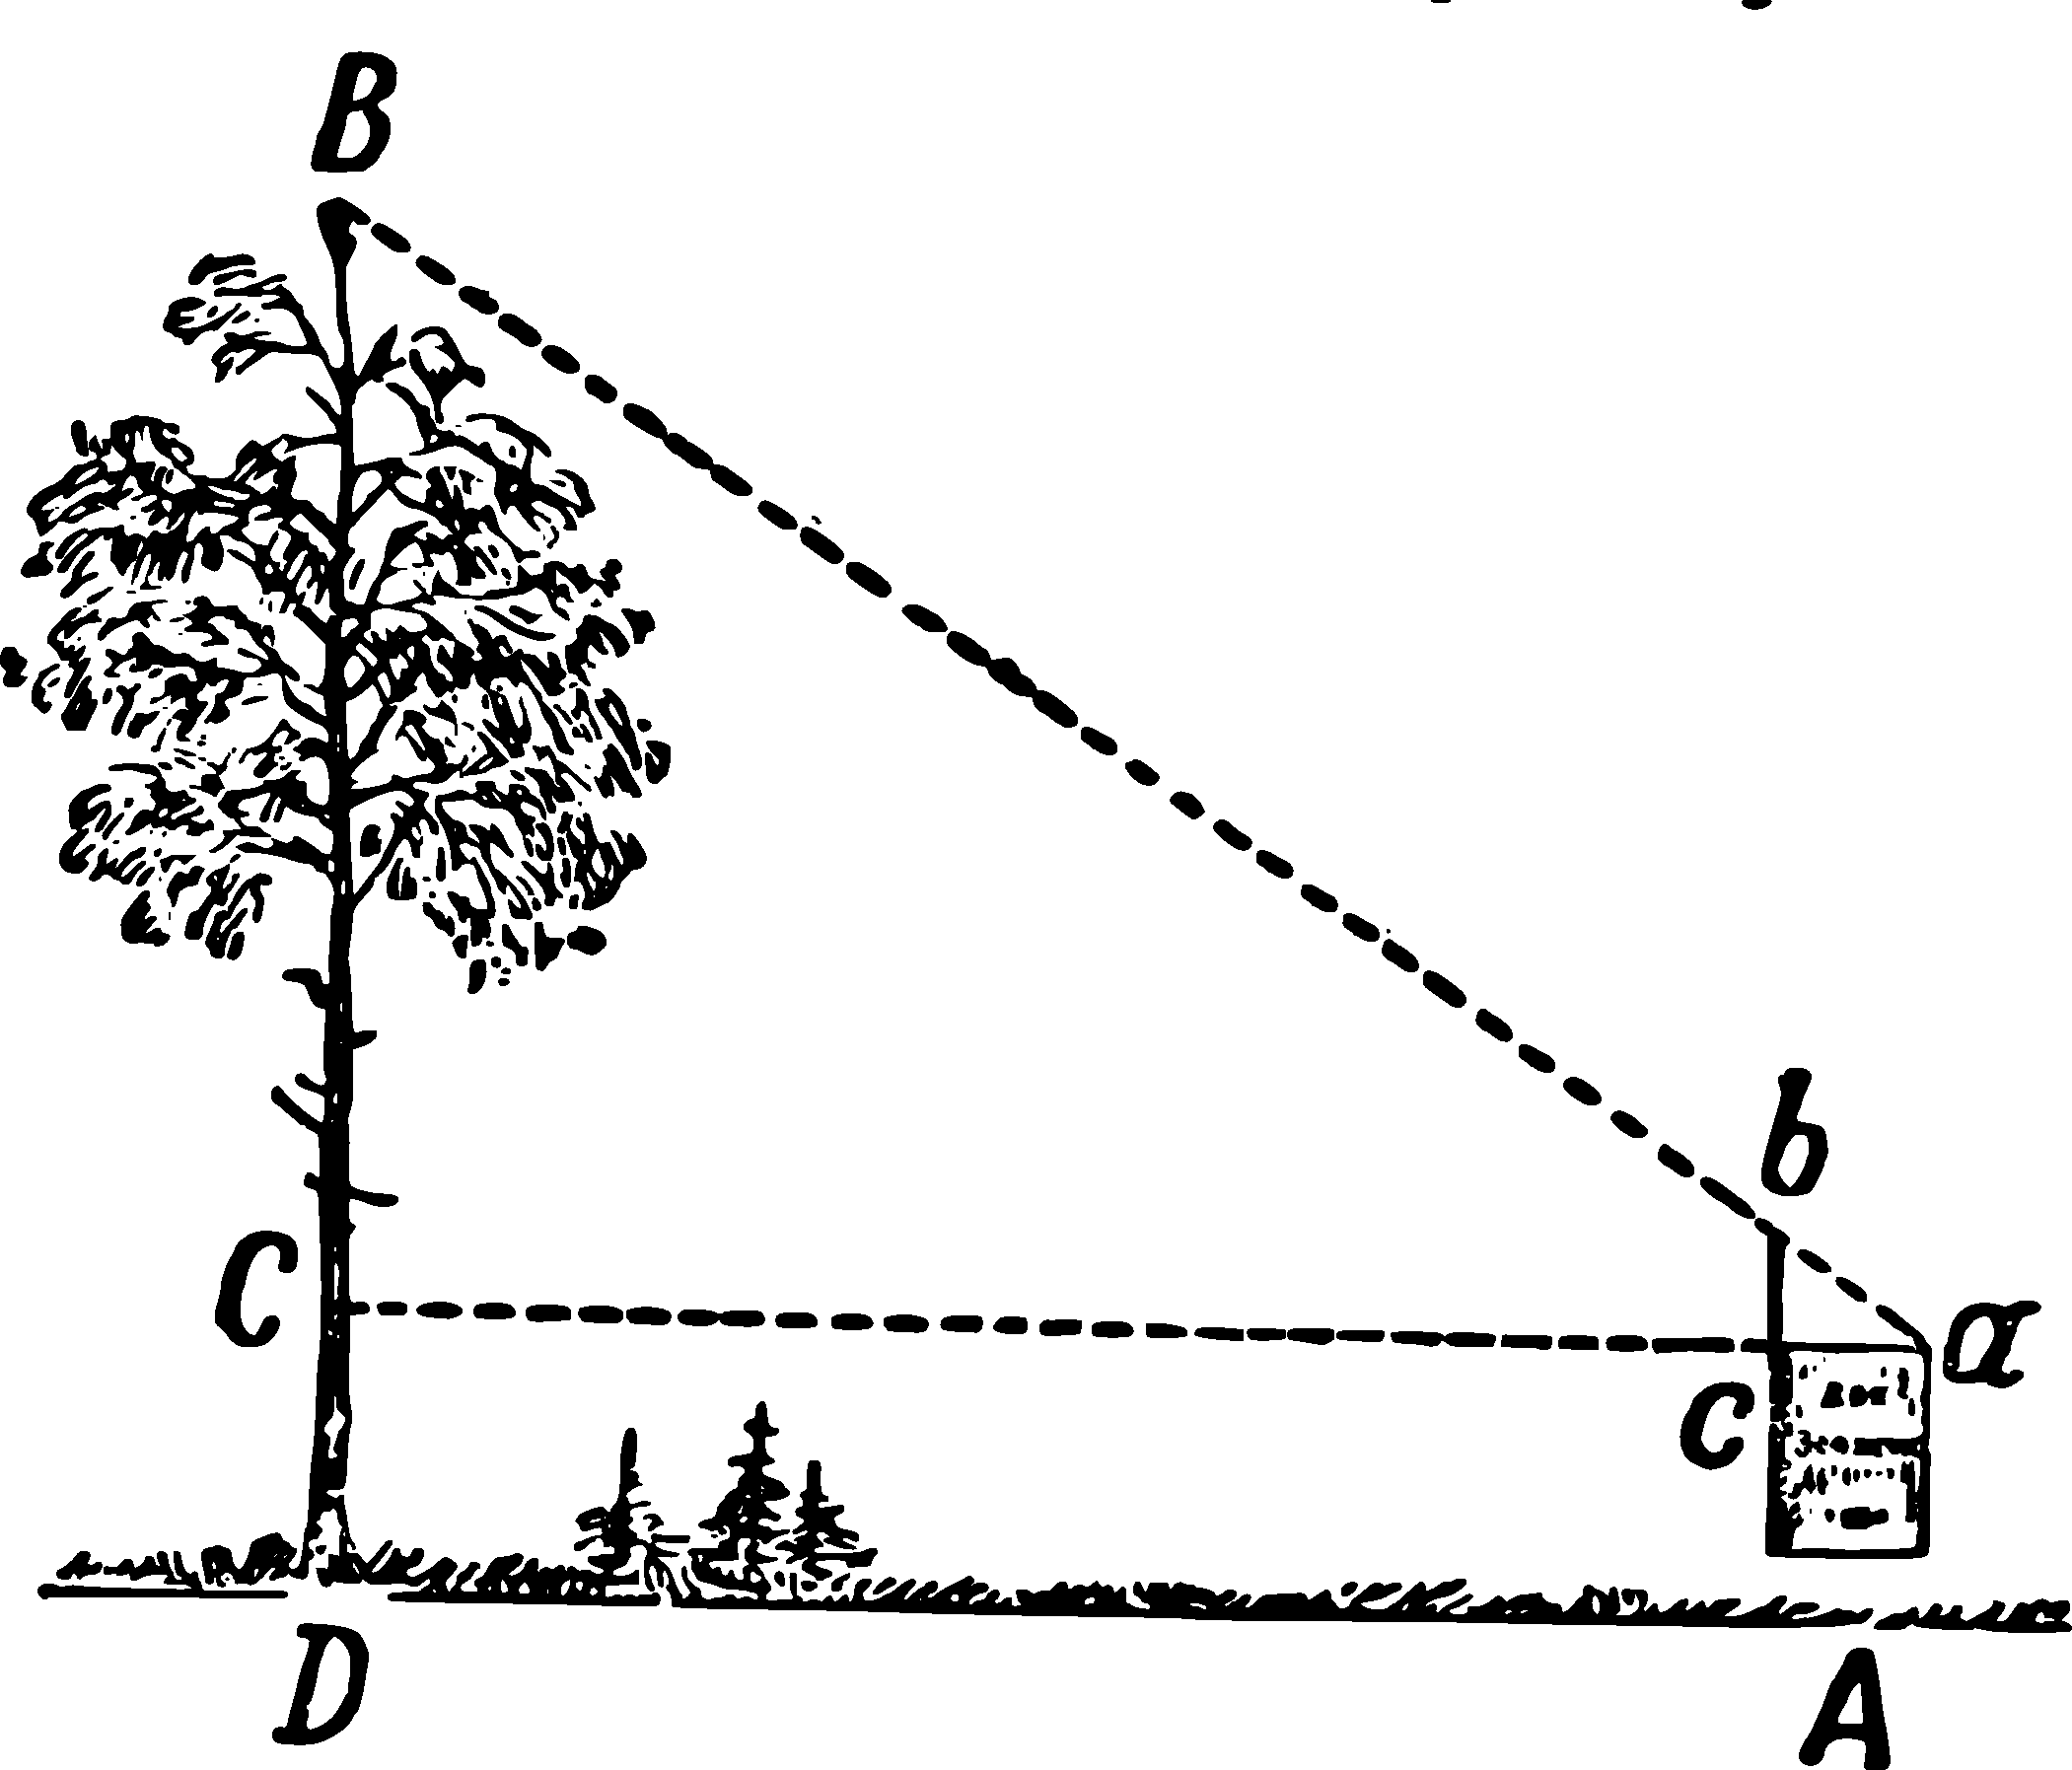
\includegraphics[width=0.6\textwidth]{figures/ch-01/fig-01-09.pdf}
\sidecaption{Height measurement using a notebook.\label{fig-01-09}}
\end{figure}

Since the width of the $ac$ book is unchanged, if you always stand at the same distance from the measured tree (for example, \SI{10}{\meter}), the height of the tree will depend only on the extended part of the pencil. Therefore, you can calculate in advance what height corresponds to a particular extension, and put these numbers on the pencil. Your notebook will then turn into a simplified altimeter, since you can use it to determine heights immediately, without calculations.





\section{Without Approaching The Tree}
\label{sec-1.6}

Sometimes it may be inconvenient to get close to the base of the tree being measured. Can its height still be determined in such a case?

Absolutely. For this purpose, a clever device has been devised, which, like the previous ones, is easy to make by yourself. Two planks, $ab$ and $cd$ (top of \figr{fig-01-10}), are fastened together at right angles so that $ab$ equals $bc$, and $bd$ equals half of $ab$. That's the whole device. 

To measure height with it, hold it in your hands, directing plank CD vertically (for which it has a plumb line with a weight), and stand precisely in two places: first (\figr{fig-01-10}) at point $A$, where the device is positioned with end $c$ up, and then at point $A'$, a bit farther away, where the device is held with end $d$ up. Point $A$ is chosen so that, looking from $a$ to the end of $a$, it is seen on the same line as the top of the tree. Point $A'$ is found so that, looking from $a'$ to point $d'$, it is seen coinciding with $B$. 

The discovery of these two points $A$ and $A'$\sidenote{These points must necessarily lie in a straight line with the base of the tree.} constitutes all the measurement because the desired part of the tree's height, $BC$, is equal to the distance $DA'$. The equality follows easily from the fact that $aC = BC$ and $a'C = 2BC$; thus,
\begin{equation*}%
a'C - aC = BC.
\end{equation*}


\begin{figure}[h!]
\centering
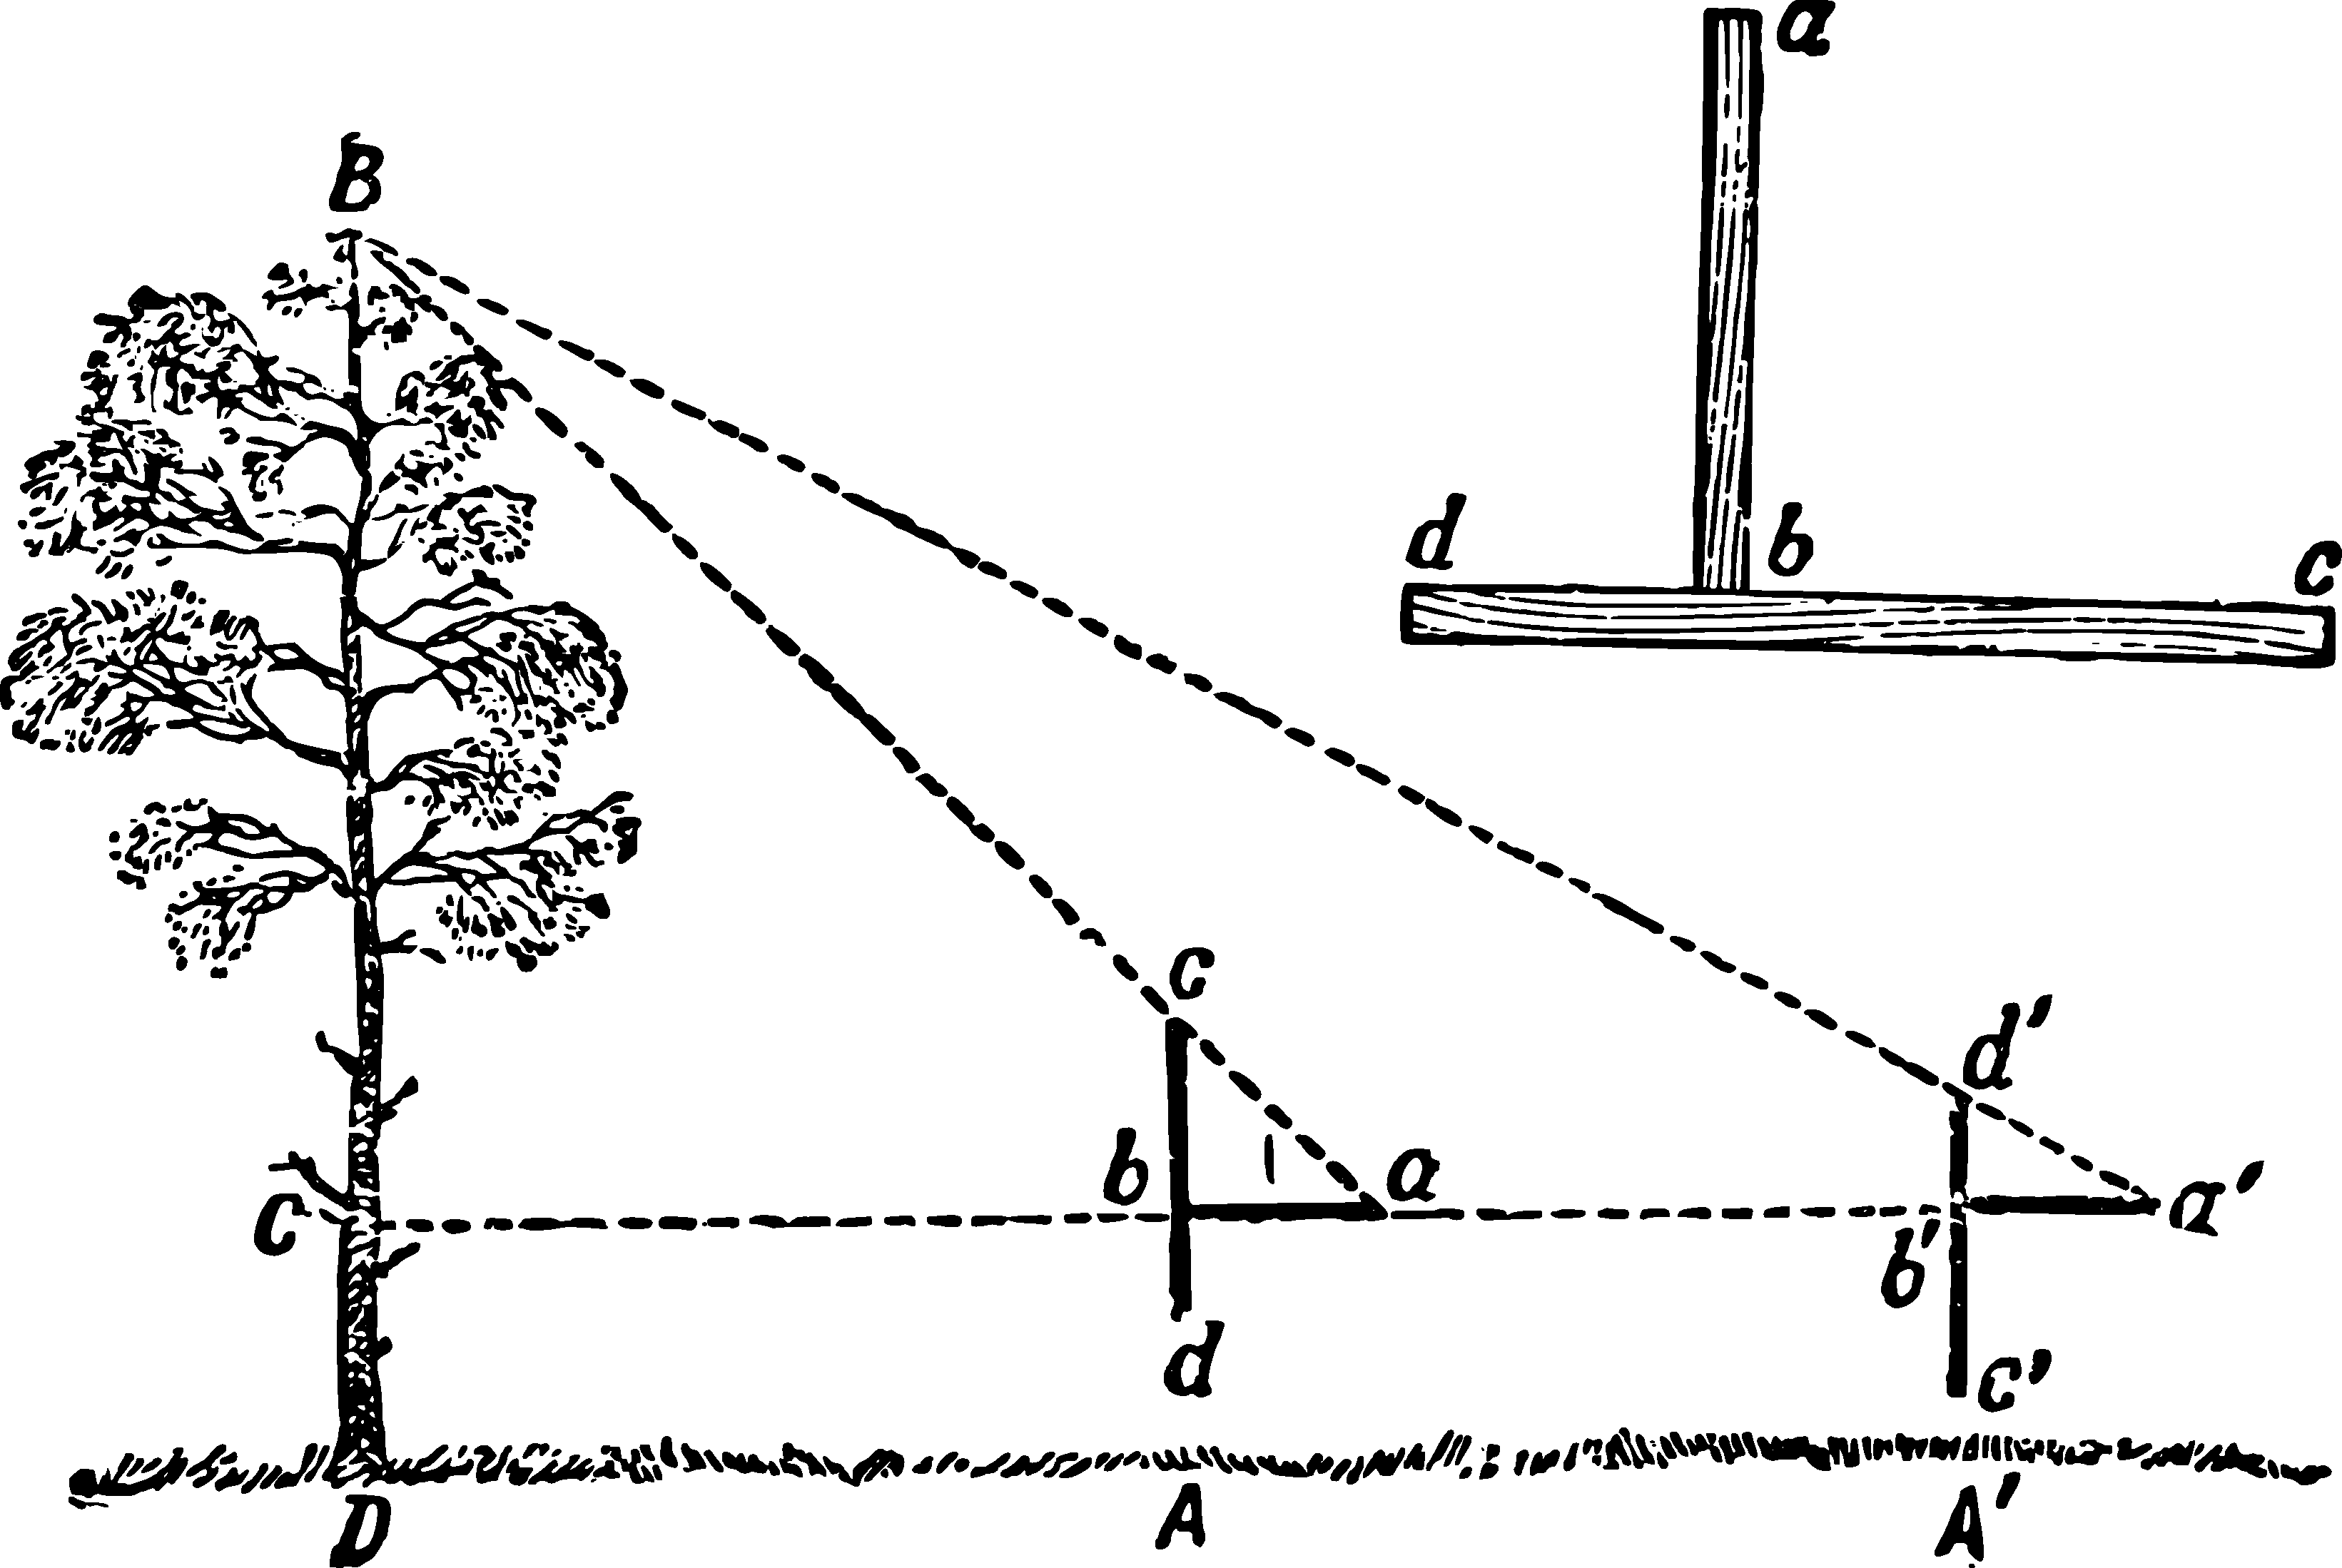
\includegraphics[width=0.8\textwidth]{figures/ch-01/fig-01-10.pdf}
\sidecaption{The use of a simple altimeter consisting of two planks.\label{fig-01-10}}
\end{figure}




You can see that using this simple device, we measure the tree's height without approaching closer than its height. It goes without saying that if it's possible to approach the trunk, it's sufficient to find just one of the points -- $A$ or $A'$ -- to determine its height.

Instead of two planks, you can use four pins, arranging them on a board properly; in this form, the ``device'' is even simpler.

%\clearpage

\section{Forest Rangers' Altimeter}
\label{sec-1.7}

It's time to explain how the ``real'' altimeters, used in practise by forest workers, are constructed. I'll describe one of these altimeters, slightly modifying it so that the device can be easily crafted at home. 

\begin{figure}[h!]
\centering
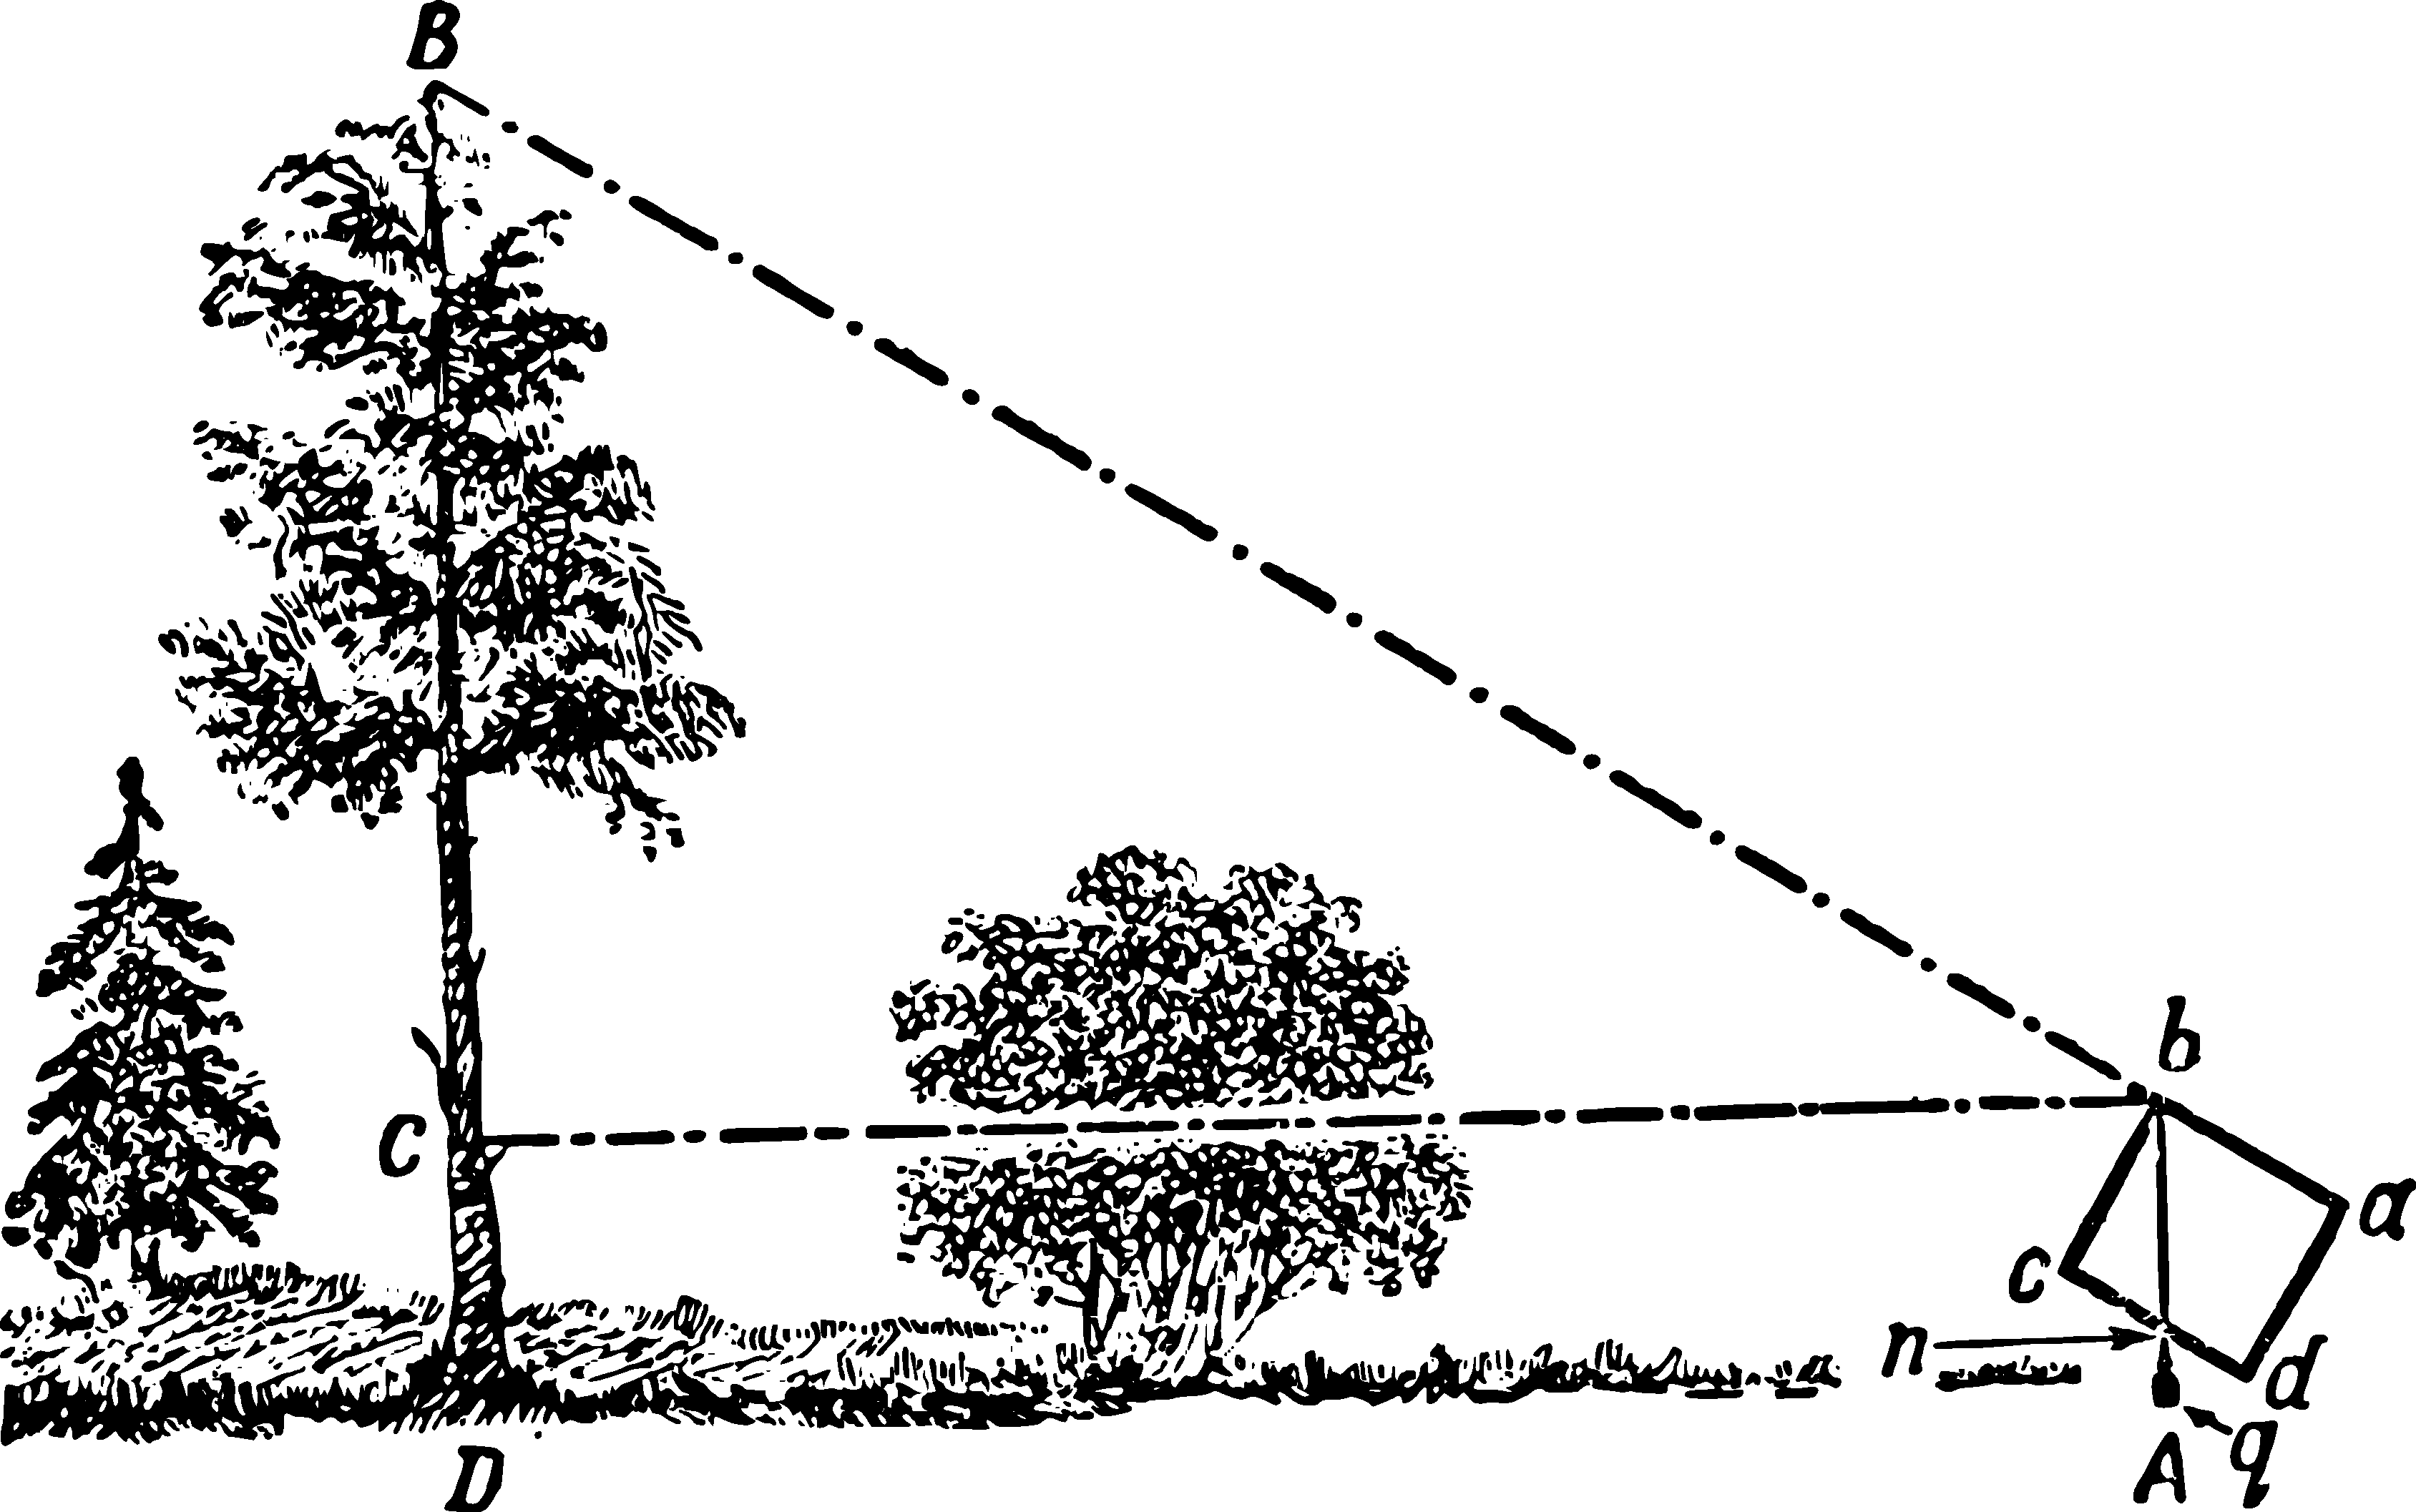
\includegraphics[width=\textwidth]{figures/ch-01/fig-01-11.pdf}
\sidecaption{The scheme of using the altimeter of foresters.\label{fig-01-11}}
\end{figure}


The essence of the device is visible in \figr{fig-01-11}. A cardboard or wooden rectangle, $abcd$, is held in the hand so that, looking along edge $ab$, the tip $B$ of the tree is in line with it. A weight, $q$, is suspended from point $b$ on a thread. We note the point $n$ where the thread intersects line $dc$. Triangles $bBC$ and $bnc$ are similar because they are both rectangular and have equal acute angles $bBC$ and $bnc$ (with corresponding parallel sides). Therefore, we can write the proportion:
\begin{align*}%
\frac{BC}{nc} & = \frac{bC}{bc}; \,\, \text{hence} \\
BC & = bC \cdot \frac{nc}{bc}.
\end{align*}
Since $bC$, $nc$, and $bc$ can be measured directly, it is easy to obtain the desired height of the tree by adding the length of the lower part $CD$ to the trunk (the height of the device above the ground). 

A few details remain to be added. If the edge of the board $bc$ is made, for example, exactly \SI{10}{\centi\meter}, and centimeter divisions are marked on edge $dc$, then the ratio $nc/bc$ will always be expressed as a decimal fraction, directly indicating what fraction of the distance $bC$ represents the height of the tree $BC$. For example, let's say the thread stops against the 7th division mark (i.e., $nc = \SI{7}{\centi\meter}$); this means that the height of the tree above eye level is 0.7 times the observer's distance from the trunk.

\begin{figure}[h!]
\centering
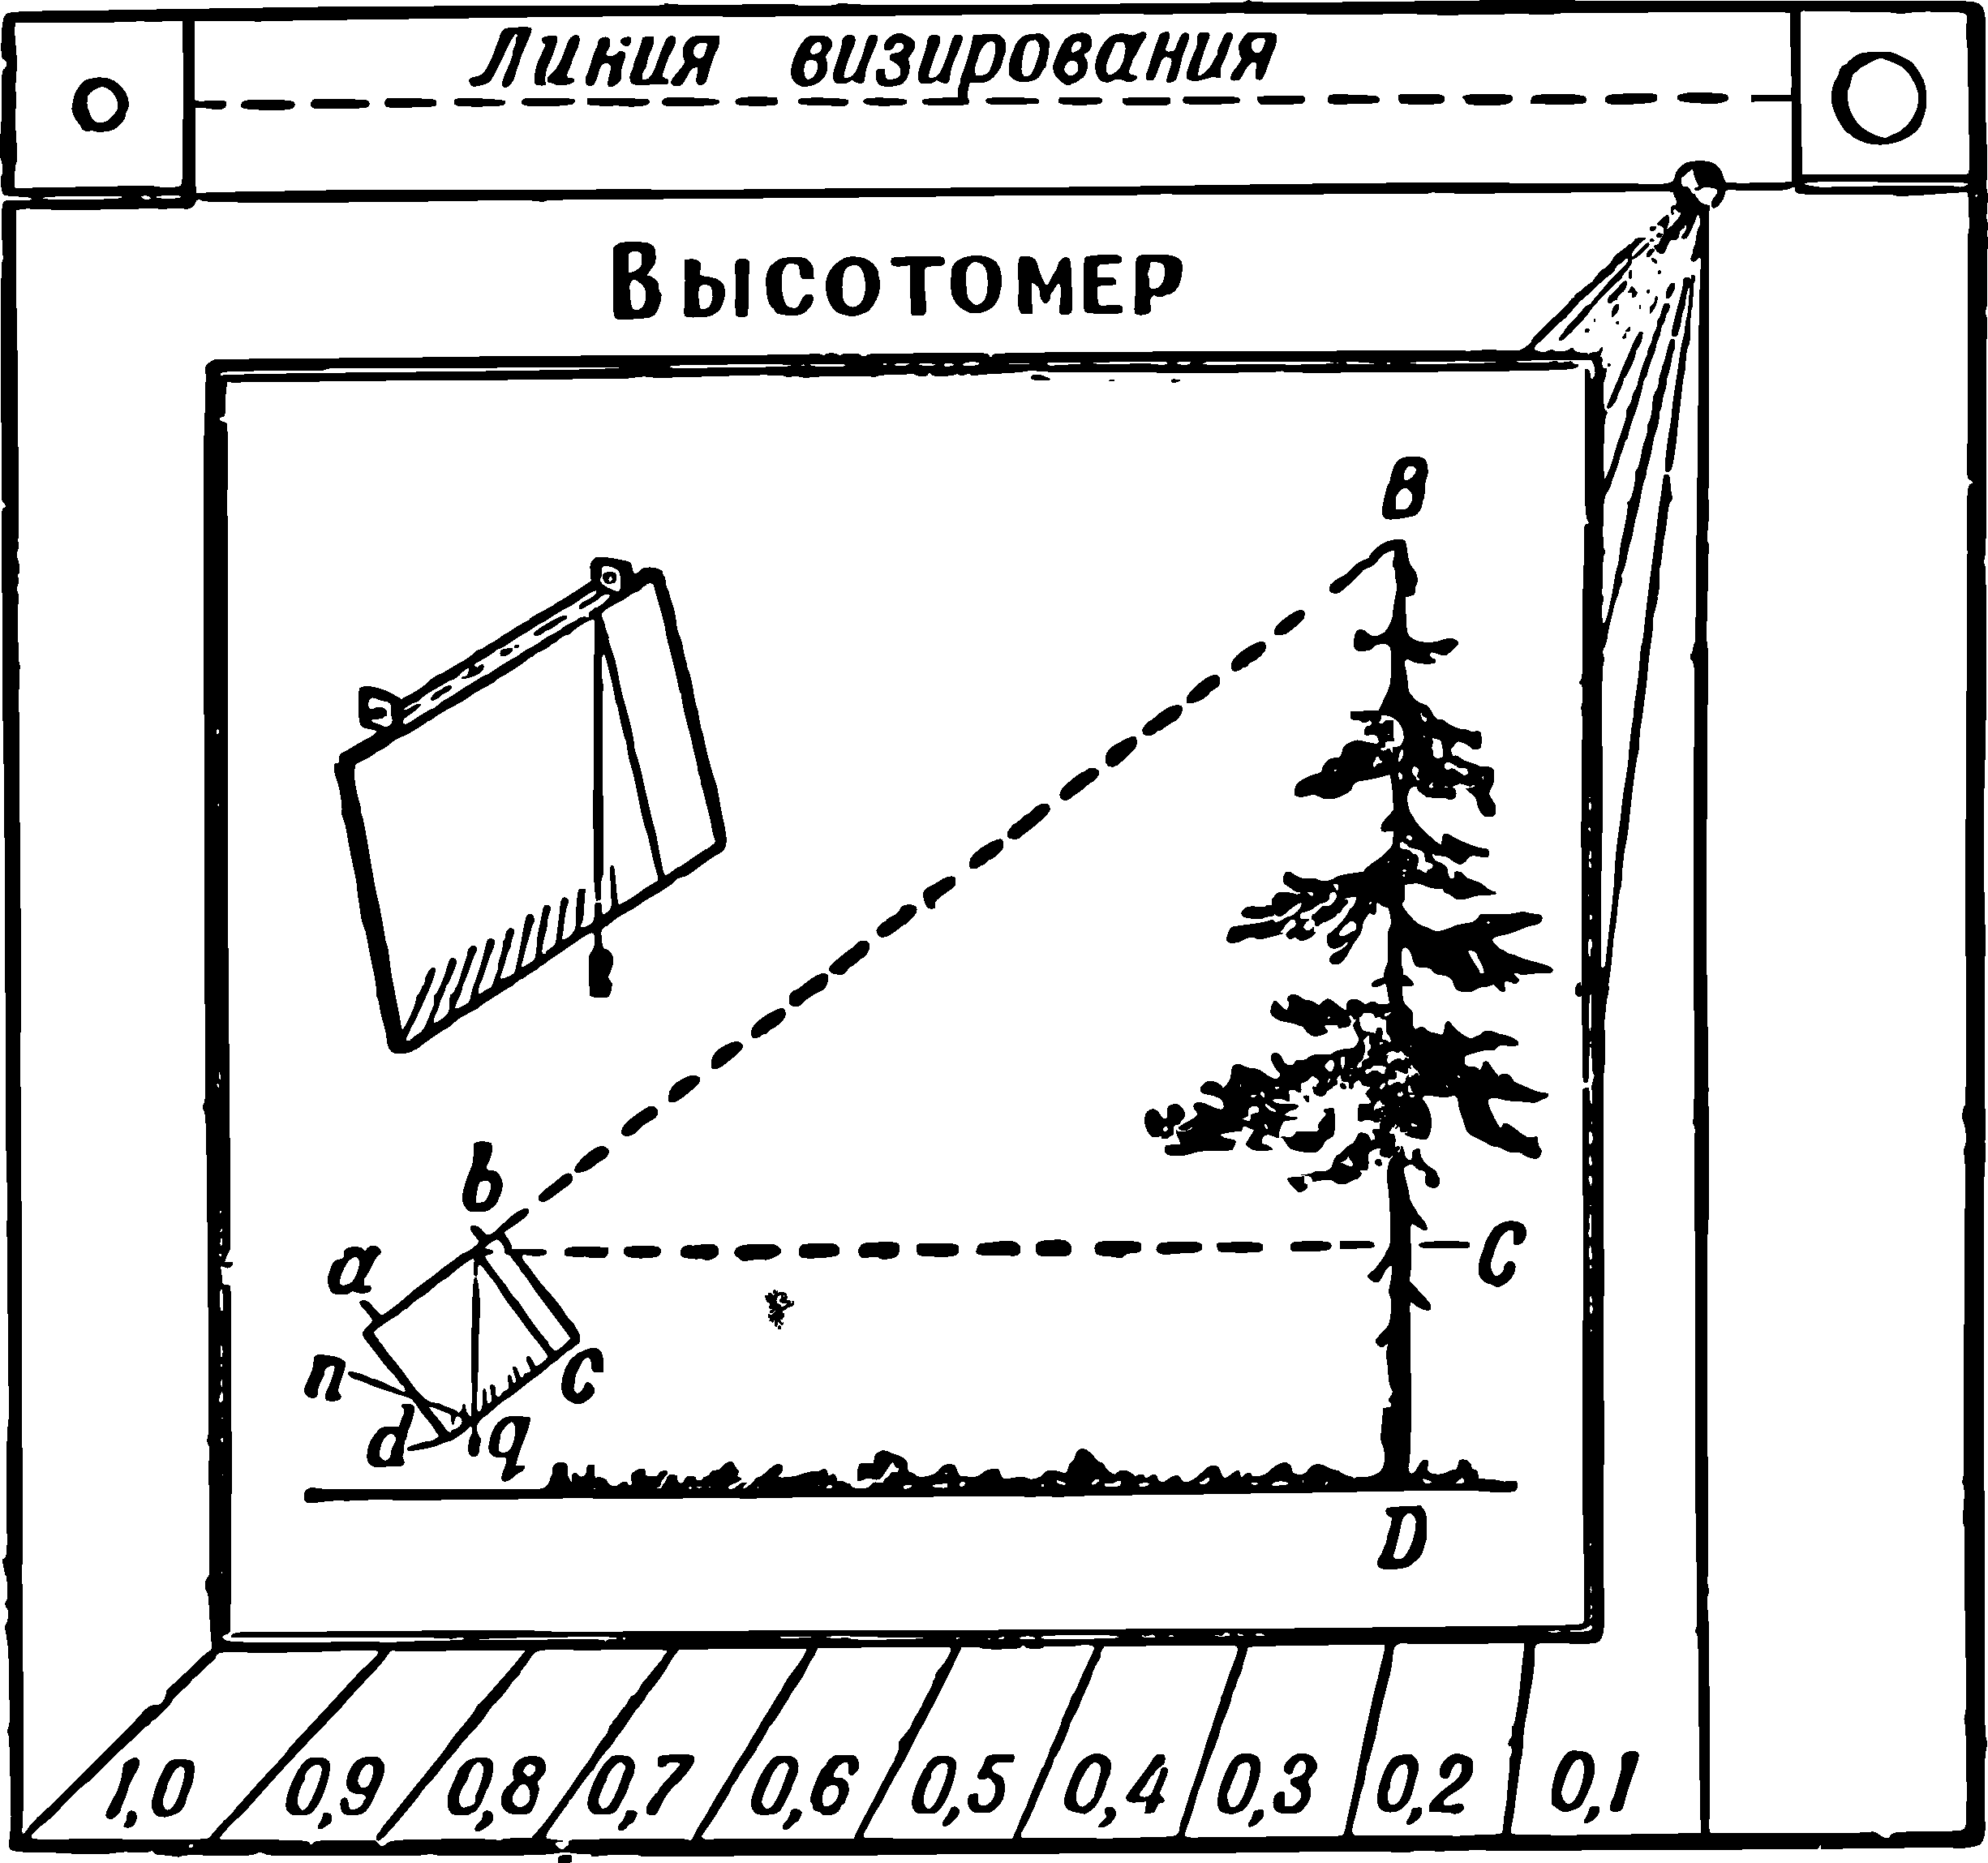
\includegraphics[width=0.7\textwidth]{figures/ch-01/fig-01-12.pdf}
\sidecaption{The forest rangers' altimeter.\label{fig-01-12}}
\end{figure}

The second improvement relates to the method of observation: to make it convenient to look along line $ab$, you can fold down two squares with holes drilled in them at the upper corners of the cardboard rectangle: one smaller one for the eye and one larger one for sighting the tree top (see \figr{fig-01-11}). Further enhancement is represented by the device shown almost to scale in \figr{fig-01-12}. It is easy and quick to make it in this form; no special skill is required. Occupying little space in the pocket, it will provide you with the ability to quickly determine the heights of encountered objects during excursions—trees, poles, buildings, and so on. (This tool is part of the \emph{Geometry in the Open Air} kit developed by the author of this book.)

%\clearpage


\ques Is it possible to use the altimeter described now to measure trees that cannot be approached closely? If possible, what should be done In such cases?


\ans The device should be aimed at the top of the tree $B$, as shown in \figr{fig-01-13}, from two points, $A$ and $A'$. 

\begin{figure}[h!]
\centering
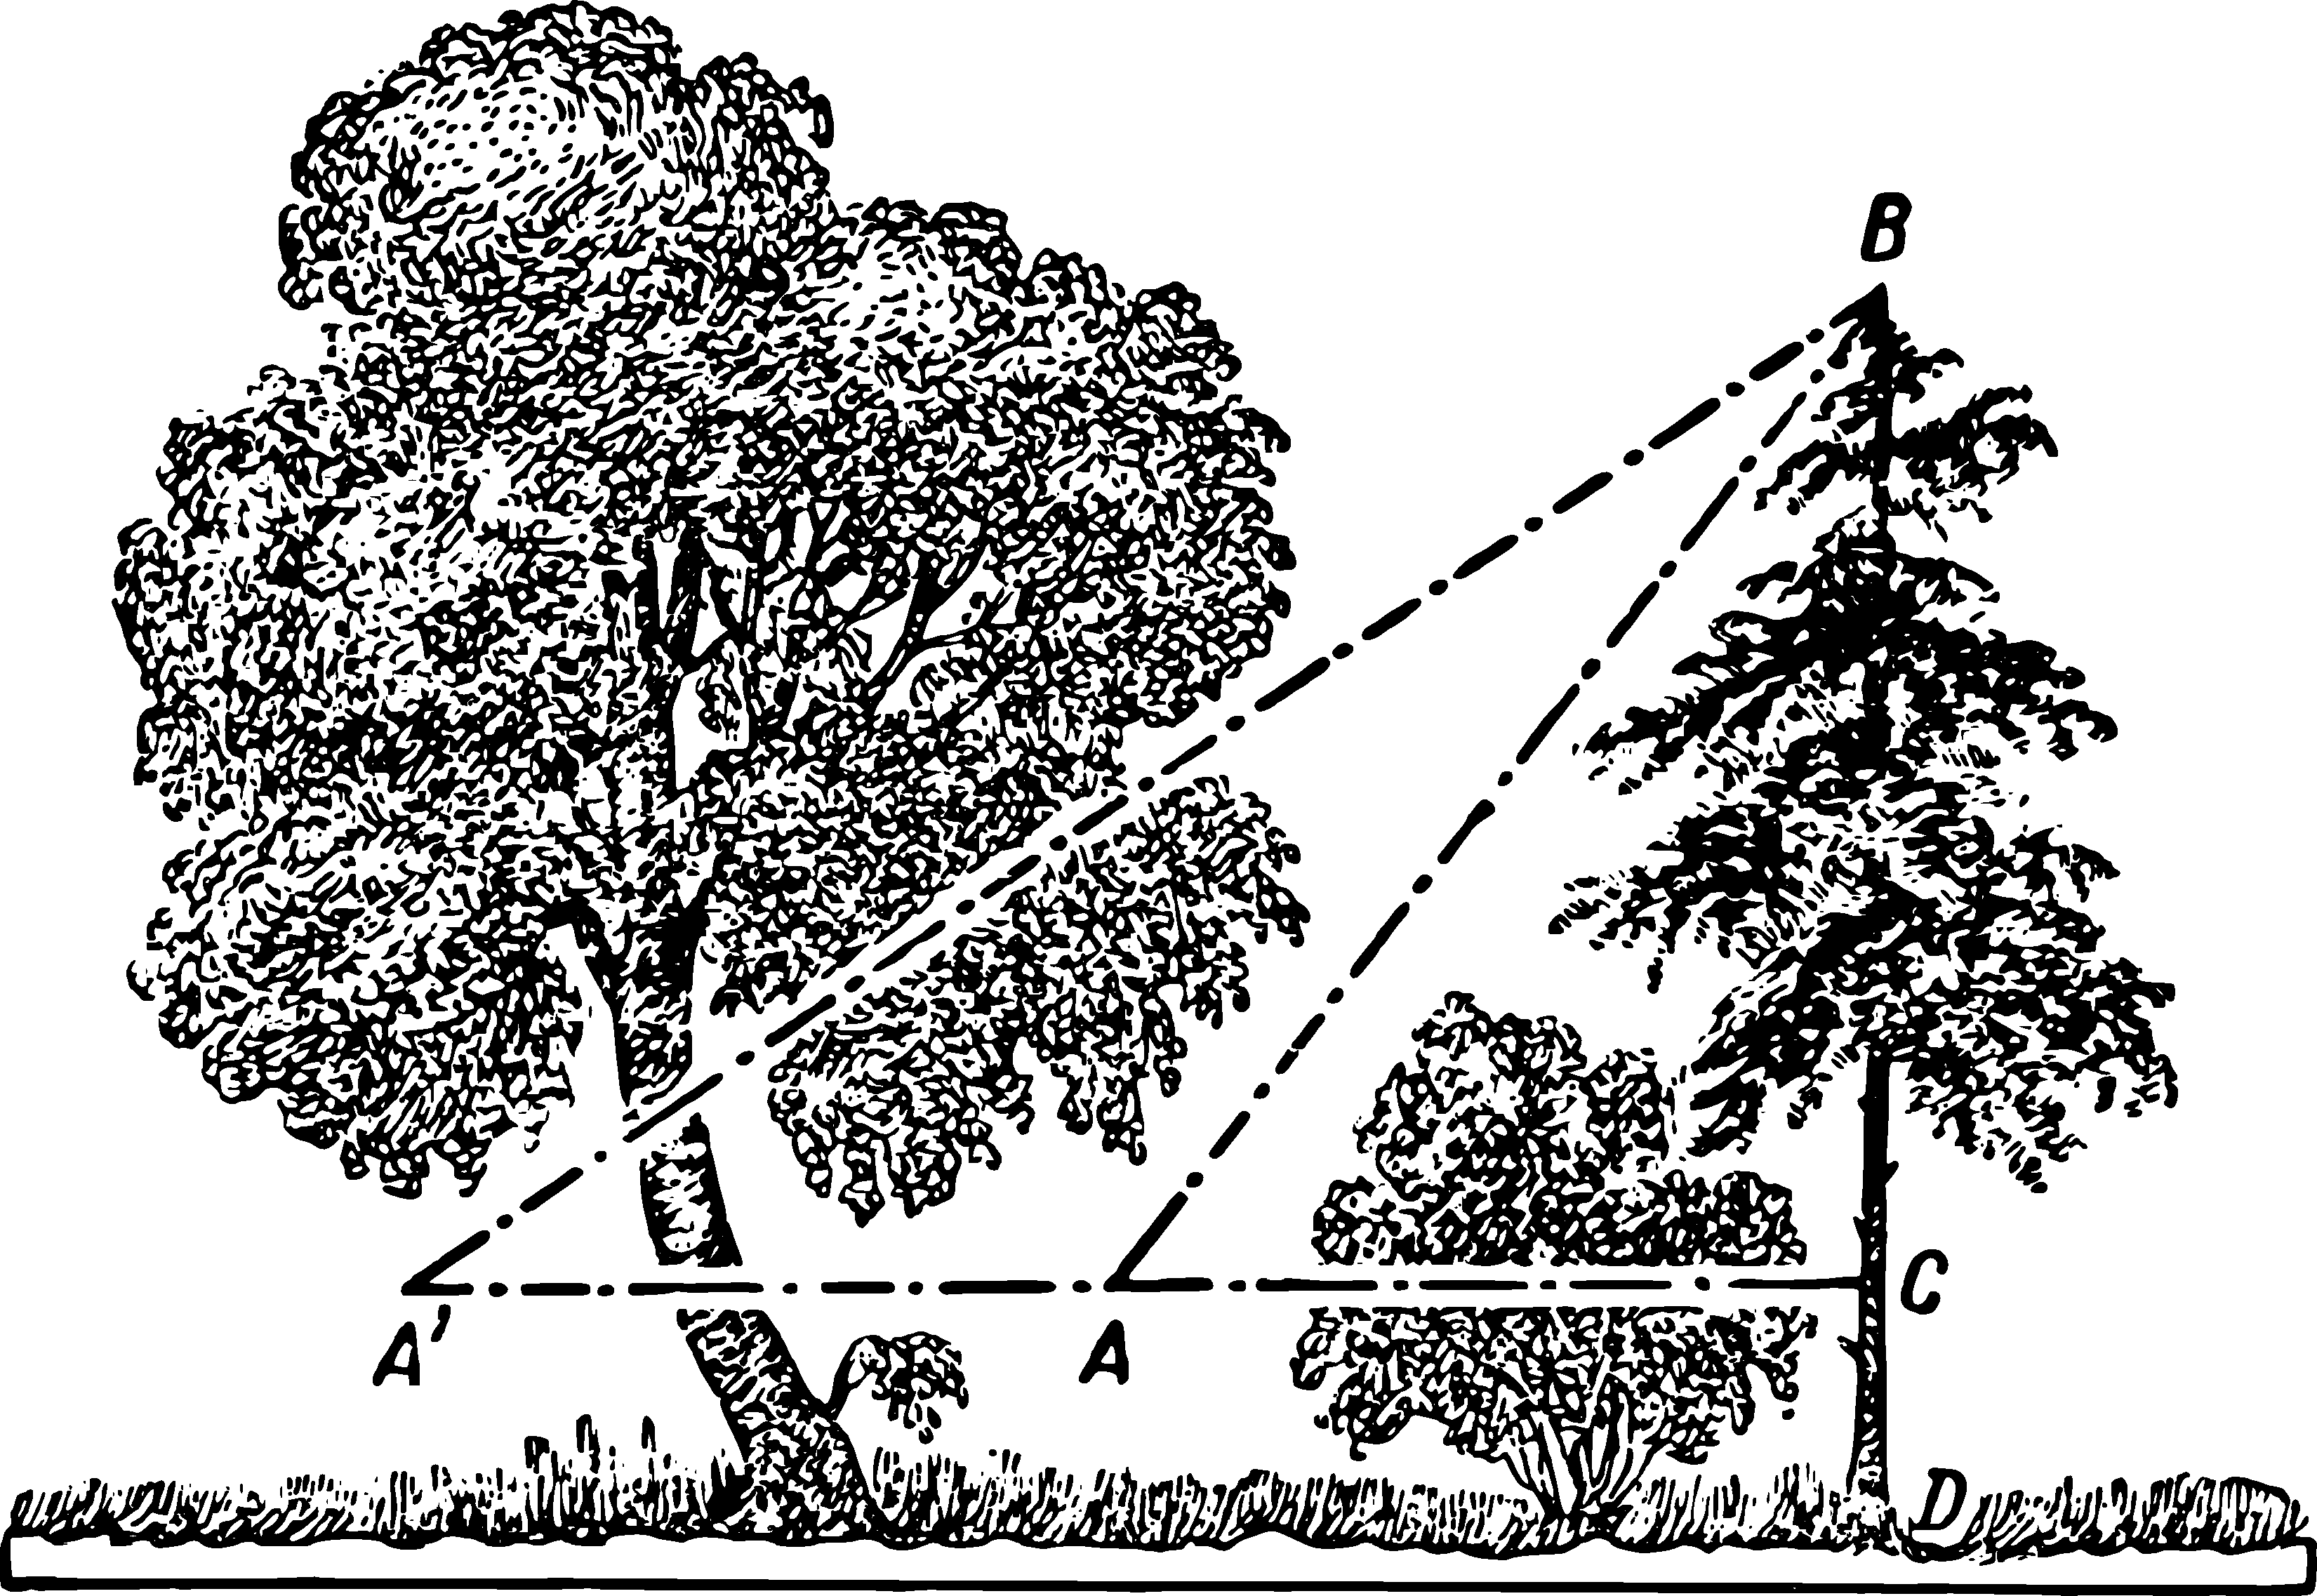
\includegraphics[width=0.9\textwidth]{figures/ch-01/fig-01-13.pdf}
\sidecaption[][-1cm]{How to measure the height of a tree without approaching it.\label{fig-01-13}}
\end{figure}

Let's say at point $A$ we determined that $BC = 0.9\,AC$, and at point $A'$ we determined that $BC = 0.4\,A'C$. Then we know that:
\begin{equation*}%
AC = \frac{BC}{0.9},\quad   A'C  = \frac{BC}{0.4} 
\end{equation*}
So that we can write
\begin{equation*}%
AA' = A'C - AC = \frac{BC}{0.4} - \frac{BC}{0.9} = \frac{25}{18} \,BC.
\end{equation*}
Hence,
\begin{align*}%
AA' & = \frac{25}{18} \,BC, \\ 
\therefore BC & = \frac{18}{25} \,AA' \\
& = 0.72 \, AA'.
\end{align*}
You can see that by measuring the distance $AA'$ between both observation points and taking a certain fraction of this value, we can determine the desired and inaccessible height.

\section{Using a Mirror}
\label{sec-1.8}


\ques Here's another unconventional method for determining the height of a tree using a mirror. At some distance (see \figr{fig-01-14}) from the tree being measured, on level ground at point $C$, place a small mirror horizontally and step back to point $D$, from where the observer can see the top of tree's point $A$ in the mirror. Then, the tree ($AB$) is as many times taller than the observer's height ($ED$) as the distance $BC$ from the mirror to the tree is greater than the distance $CD$ from the mirror to the observer. Why?

\begin{figure}[h!]
\centering
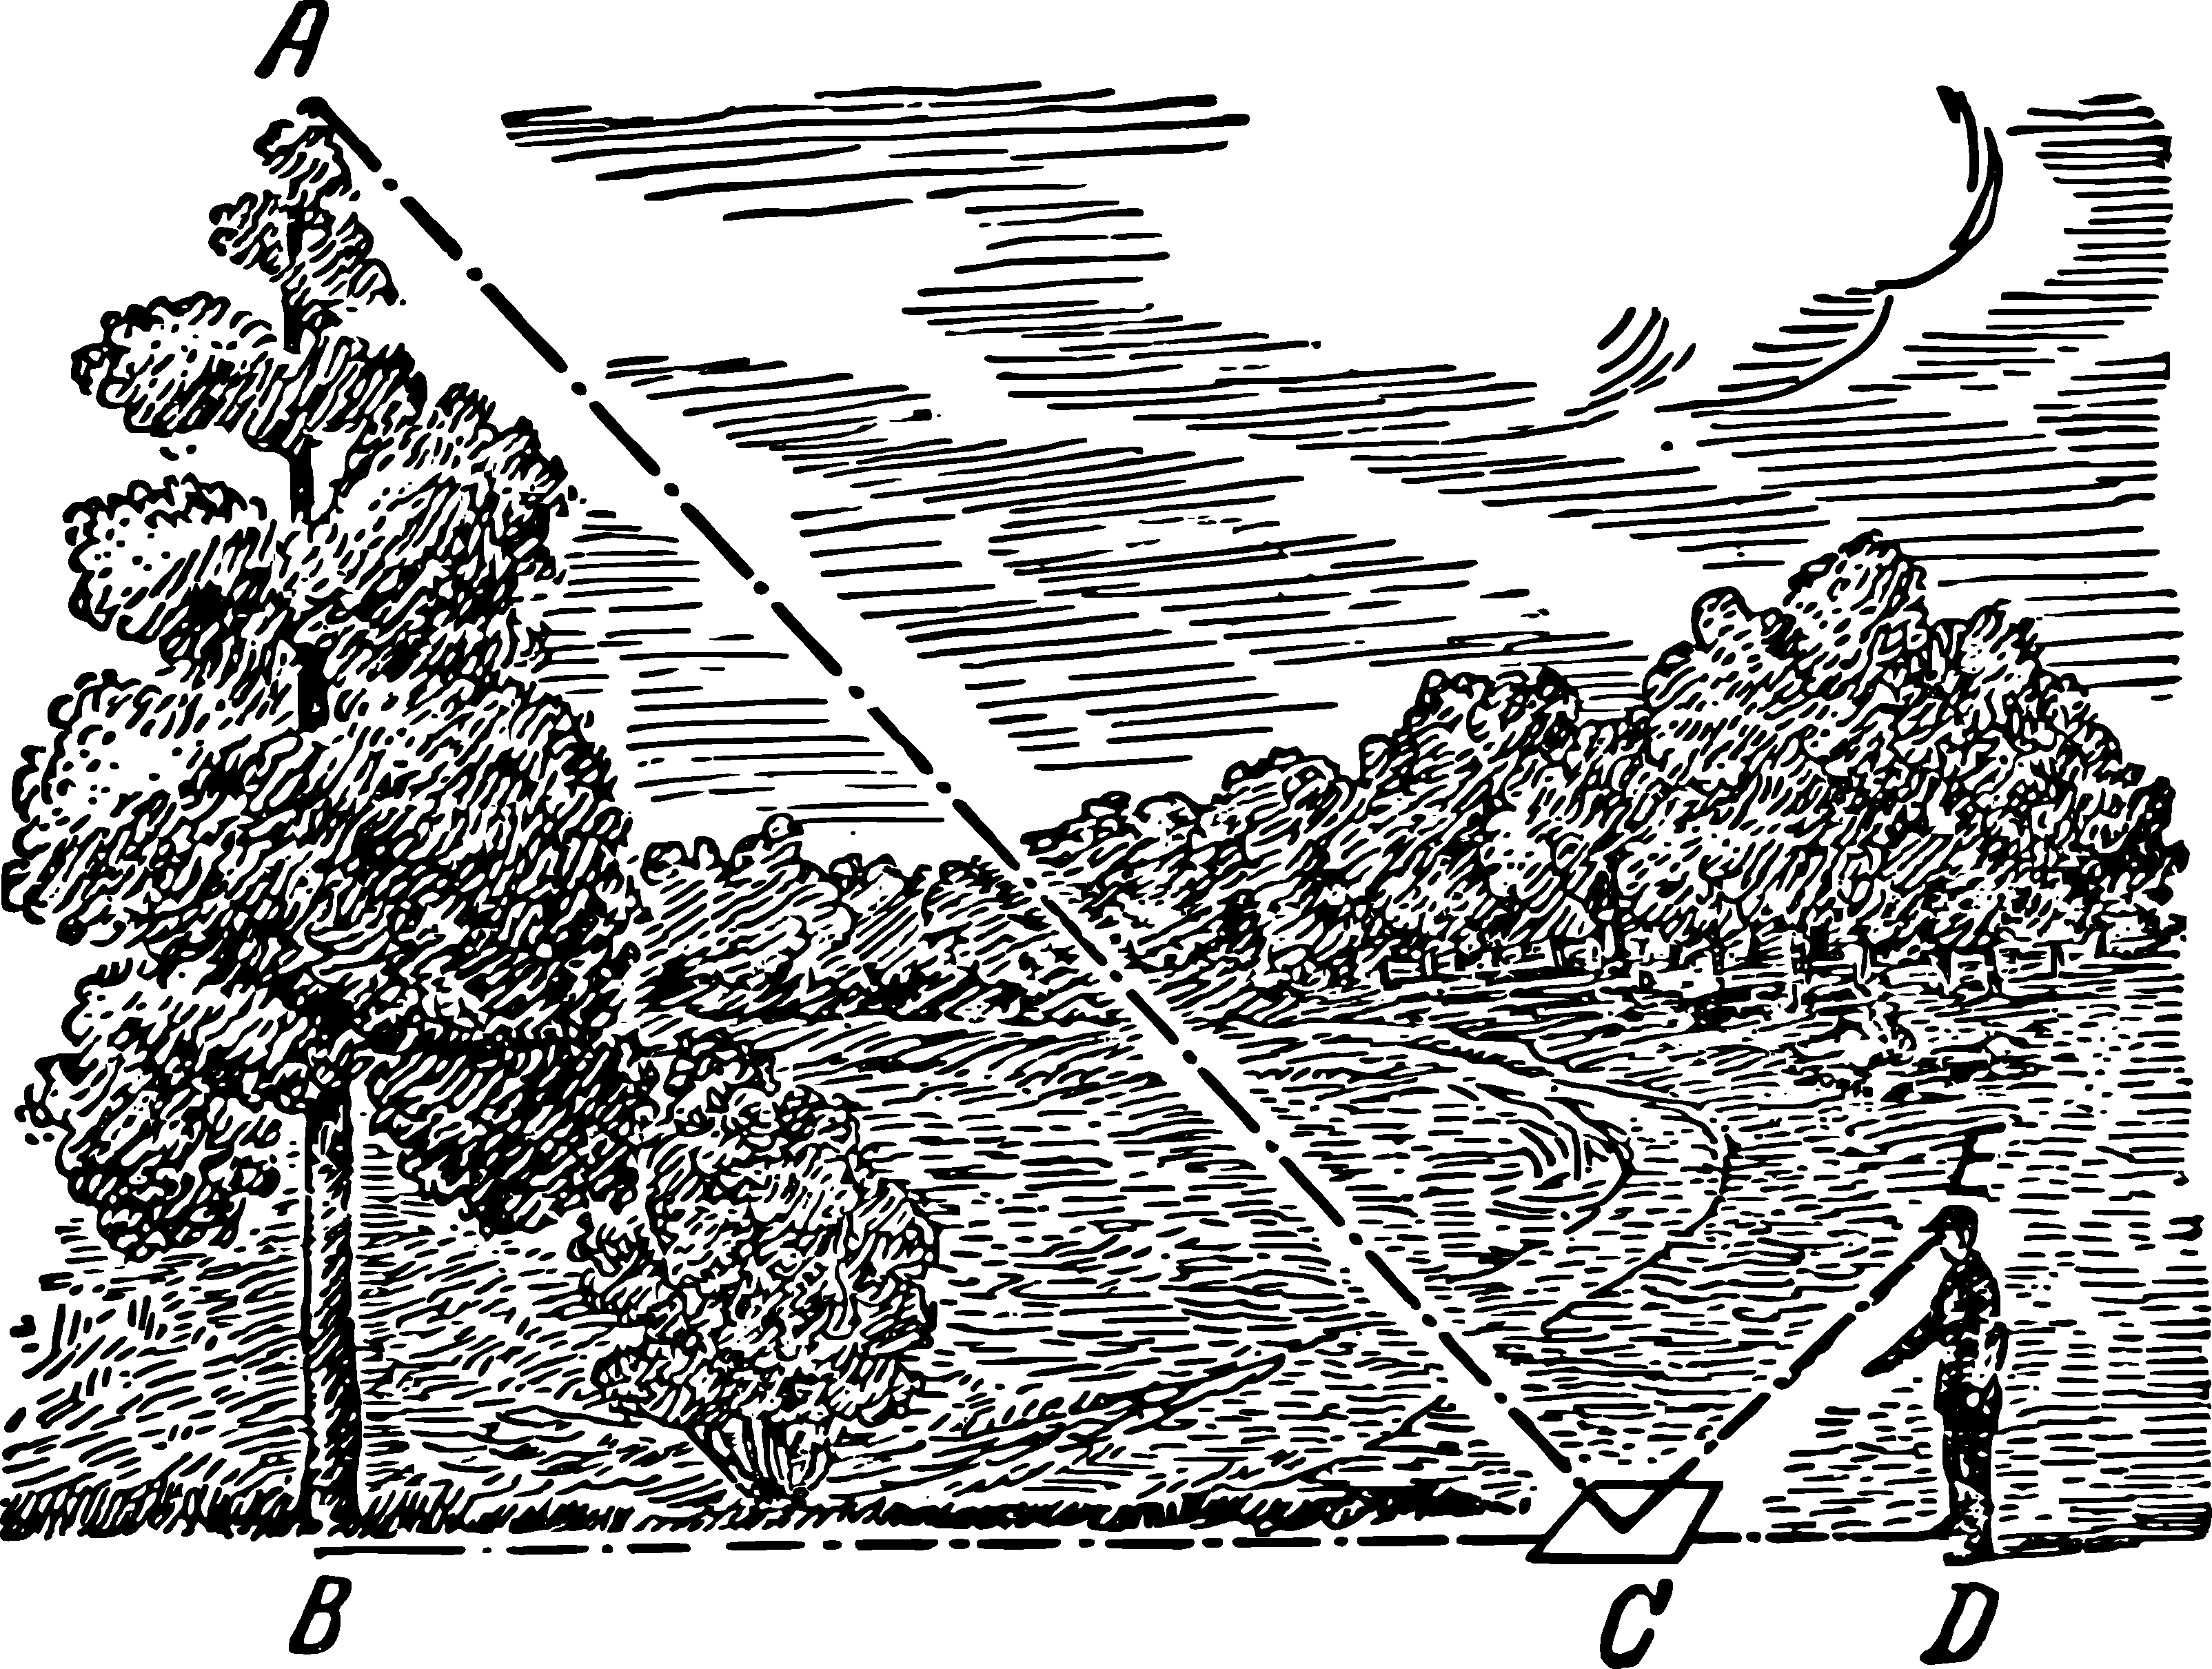
\includegraphics[width=0.9\textwidth]{figures/ch-01/fig-01-14.pdf}
\sidecaption[][0cm]{Height measurement using a mirror.\label{fig-01-14}}
\end{figure}


\ans The method is based on the law of reflection of light. The top $A$ (\figr{fig-01-15}) is reflected at point $A'$ in such a way that $AB = A'B$. From the similarity of triangles $BCA'$ and $CED$, it follows that 
\begin{equation*}%
\frac{A'B}{ED} = \frac{BC}{CD}. 
\end{equation*}
In this, simply replace $A'B$ with $AB$ to justify the relationship stated in the problem. This convenient and effortless method can be applied in any weather, but not in dense vegetation, only to a solitary tree.
\begin{marginfigure}[-4cm]%[h!]
\centering
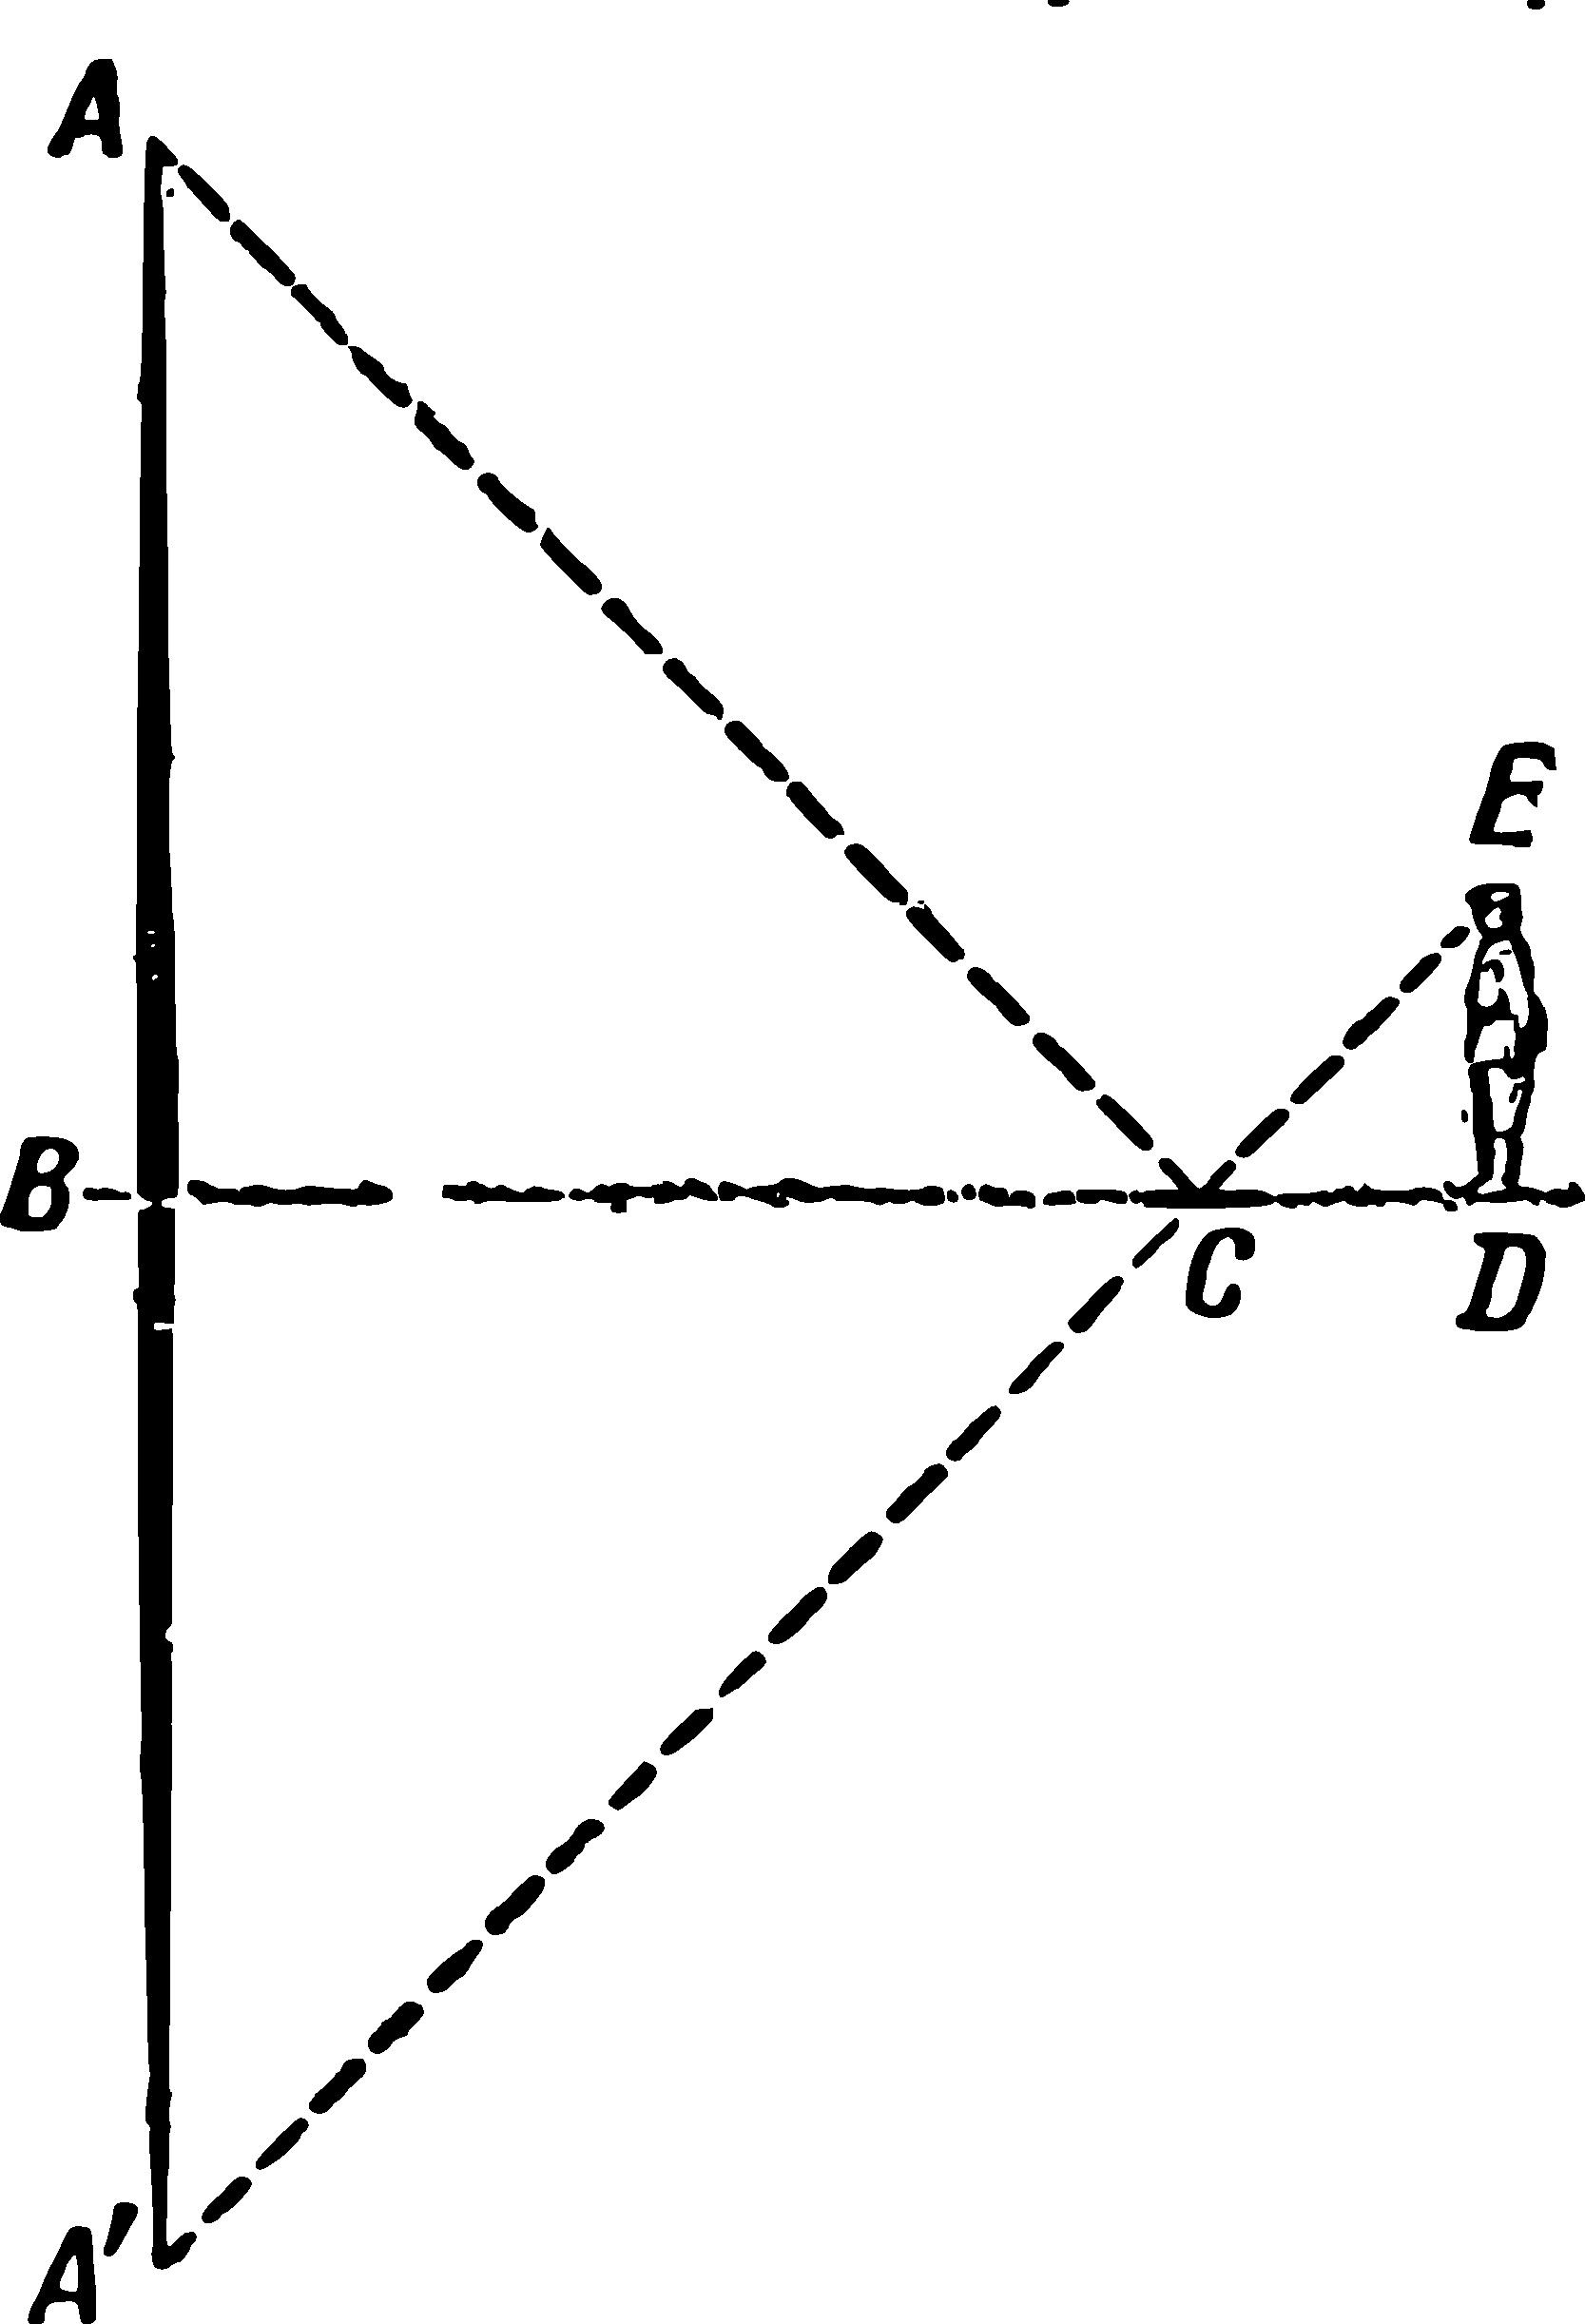
\includegraphics[width=0.9\textwidth]{figures/ch-01/fig-01-15.pdf}
\sidecaption{Geometric construction for the method of measuring the height using a mirror.\label{fig-01-15}}
\end{marginfigure}

%\clearpage 

\ques However, what should be done when it is impossible to approach the tree being measured closely for some reason?\\

\ans This is an ancient problem dating back over 500 years. It is discussed by the medieval mathematician Antonius de Cremona in his work \emph{On Practical Land Measurement} (1400).


The problem is solved by the dual application of the method described earlier -- placing the mirror in two locations. By making the appropriate construction, it is easy to deduce from the similarity of triangles that the sought-after height of the tree is equal to the observer's eye level multiplied by the ratio of the distance between the mirror positions to the difference in distances from the mirror to the observer.

Before concluding the discussion on measuring the height of trees, I propose to the reader another ``forest'' problem.

\section{Two Pines}
\label{sec-1.9}


\ques Two pine trees grow 40 meters apart. You measured their heights: one turned out to be 31 meters tall, while the other, younger one, is only 6 meters tall. Can you calculate the distance between their tops?

\begin{figure}[h!]
\centering
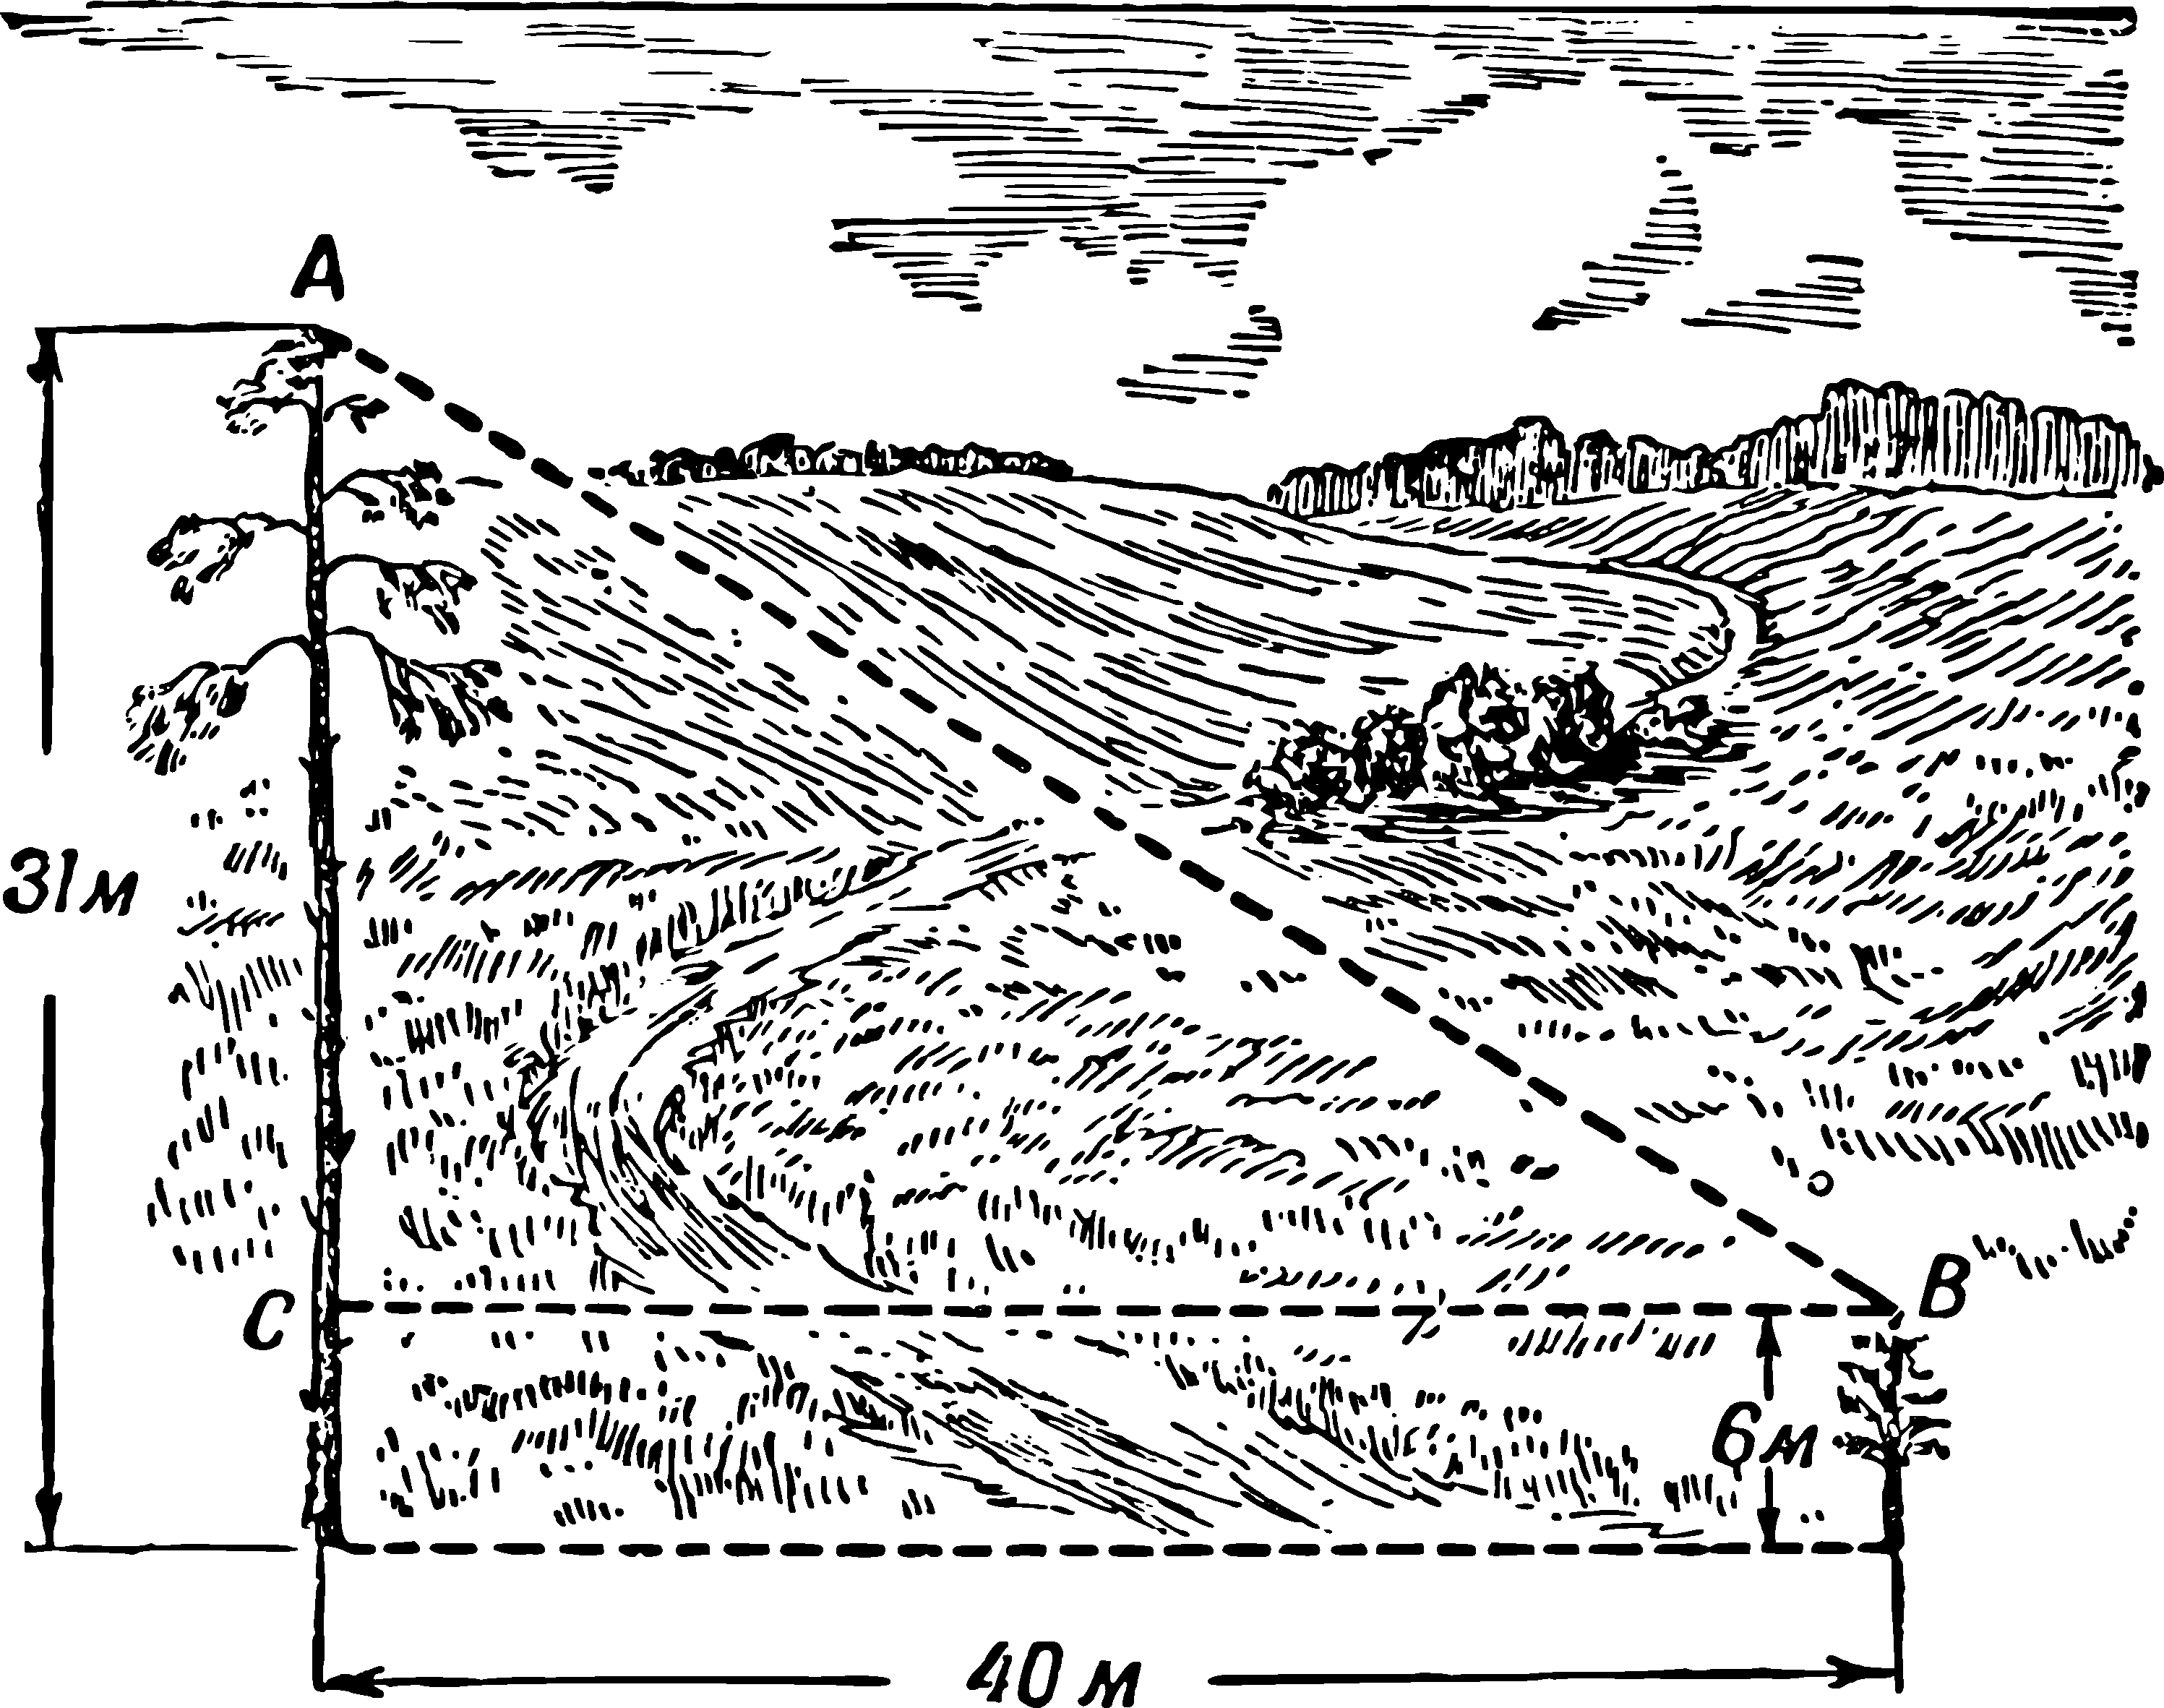
\includegraphics[width=0.9\textwidth]{figures/ch-01/fig-01-16.pdf}
\sidecaption{What is the distance between the tops of the pines?\label{fig-01-16}}
\end{figure}

\ans The desired distance between the tops of the pine trees (see \figr{fig-01-16}) according to the Pythagorean theorem is
\begin{equation*}%
\sqrt{40^{2} + 25^{2}} = \SI{47}{\meter}.
\end{equation*}



\section{The shape of the tree trunk}
\label{sec-1.10}

Now you can already, walking through the forest, determine -- in almost half a dozen different ways -- the height of any tree. It will probably be interesting for you to determine its volume as well, calculate how many cubic meters of wood it contains, and at the same time weigh it. To find out if, for example, it would be possible to take away such a trunk on one cart. Both of these tasks are no longer as simple as determining height; experts have not found ways to accurately resolve it and are content with only a more or less approximate estimate. Even for a felled trunk, which lies in front of you cleared of branches, the task is far from easy.

The thing is, a tree trunk, even the smoothest one without bulges, does not represent either a cylinder, a complete cone, a truncated cone, or any other geometric solid whose volume we can calculate using formulas. The trunk is certainly not a cylinder — it tapers towards the top (it has ``runoff'', as foresters say) — but it is also not a cone because its ``generating line'' is not a straight line, but a curve, and moreover, not a circular arc, but some other curve, convex towards the axis of the tree.\sidenote[][-5cm]{The curve that fits closest to this is called the ``semicubical parabola'' $(y^3 = ax^2)$; the solid obtained by rotating this parabola is called a ``neiloid'' (named after the ancient mathematician Neil, who found a way to determine the length of the arc of such a curve). The shape of a tree trunk grown in the forest approximates that of a neiloid. Calculating the volume of a neiloid is done using advanced mathematical techniques.}

Therefore, a more or less accurate calculation of the volume of a tree trunk can only be done using the tools of integral calculus. To some readers, it may seem strange that the measurement of a simple log requires resorting to the services of higher mathematics. Many think that higher mathematics is only relevant to some special subjects, whereas in everyday life, only elementary mathematics is applicable. This is completely incorrect: one can fairly accurately calculate the volume of a star or a planet using elements of geometry, whereas an exact calculation of the volume of a long log or a beer barrel is impossible without analytical geometry and integral calculus.

However, our book does not assume that the reader is familiar with higher mathematics; therefore, here we will have to be content with only an approximate calculation of the volume of the trunk. We will assume that the volume of the trunk is more or less close either to the volume of a truncated cone, or -- for a trunk with a pointed end — to the volume of a complete cone, or, finally, -- for short logs — to the volume of a cylinder. The volume of each of these three solids can be easily calculated. Could we find a formula for the volume that would be suitable for all three of these named solids for the sake of consistency in calculation? Then we would approximately calculate the volume of the trunk without caring about what it resembles more — a cylinder or a cone, complete or truncated.


\section{Universal Formula}
\label{sec-1.11}

Such a formula exists; moreover, it is not only suitable for cylinders, complete and truncated cones, but also for all kinds of prisms, pyramids complete and truncated, and even for spheres. Here is this remarkable formula, known in mathematics as Simpson's formula:
\begin{equation*}
v = \frac{h}{6}\, (b_{1} + 4b_{2} + b_{3})
\end{equation*}
where $h$ is the height of the solid, $b_{1}$ is the area of the lower base, $b_{2}$ is the area of the middle section\sidenote[][-2cm]{ That is, the cross-sectional area of the body in the middle of its height.}, $b_{3}$ is the area of the upper base.

\ques Prove that with this formula, one can calculate the volume of the following seven geometric solids: prism, pyramid complete, pyramid truncated, cylinder, cone complete, cone truncated, sphere.

\ans It is very easy to verify the correctness of this formula by simply applying it to the listed solids. Then, we obtain for the prism and cylinder (see \figr{fig-01-17}~\drkgry{a}):
\begin{equation*}%
v = \frac{h}{6}\, (b_{1} + 4b_{2} + b_{3}) = b_{1}h;
\end{equation*}
for the pyramid and cone (see \figr{fig-01-17}~\drkgry{b}):
\begin{equation*}%
v = \frac{h}{6}\, (b_{1} + 4\frac{b_{2}}{4} + 0) = \frac{b_{1}h}{3};
\end{equation*}
for the truncated cone (see \figr{fig-01-17}~\drkgry{c}):
\begin{align*}%
v & = \frac{h}{6}\, \left[ \pi R^{2} + 4 \pi \frac{(R + r)^{2}}{2} + \pi r^{2} \right] \\ 
& = \frac{h}{6}\, \left[ \pi R^{2} + \pi R^{2} + 2 \pi Rr +  \pi r^{2} + \pi r^{2} \right] \\ 
& = \frac{\pi h}{3}\, \left[ R^{2} + Rr + r^{2}\right],
\end{align*}
for the truncated pyramid, the proof proceeds similarly; finally, for the sphere (see \figr{fig-01-17}~\drkgry{d}):
\begin{equation*}%
v = \frac{2R}{6}\, (0 + 4 \pi R^{2}{4} + 0) = \frac{4}{3}\pi R^{3}.
\end{equation*}

\begin{figure}[h!]
\centering
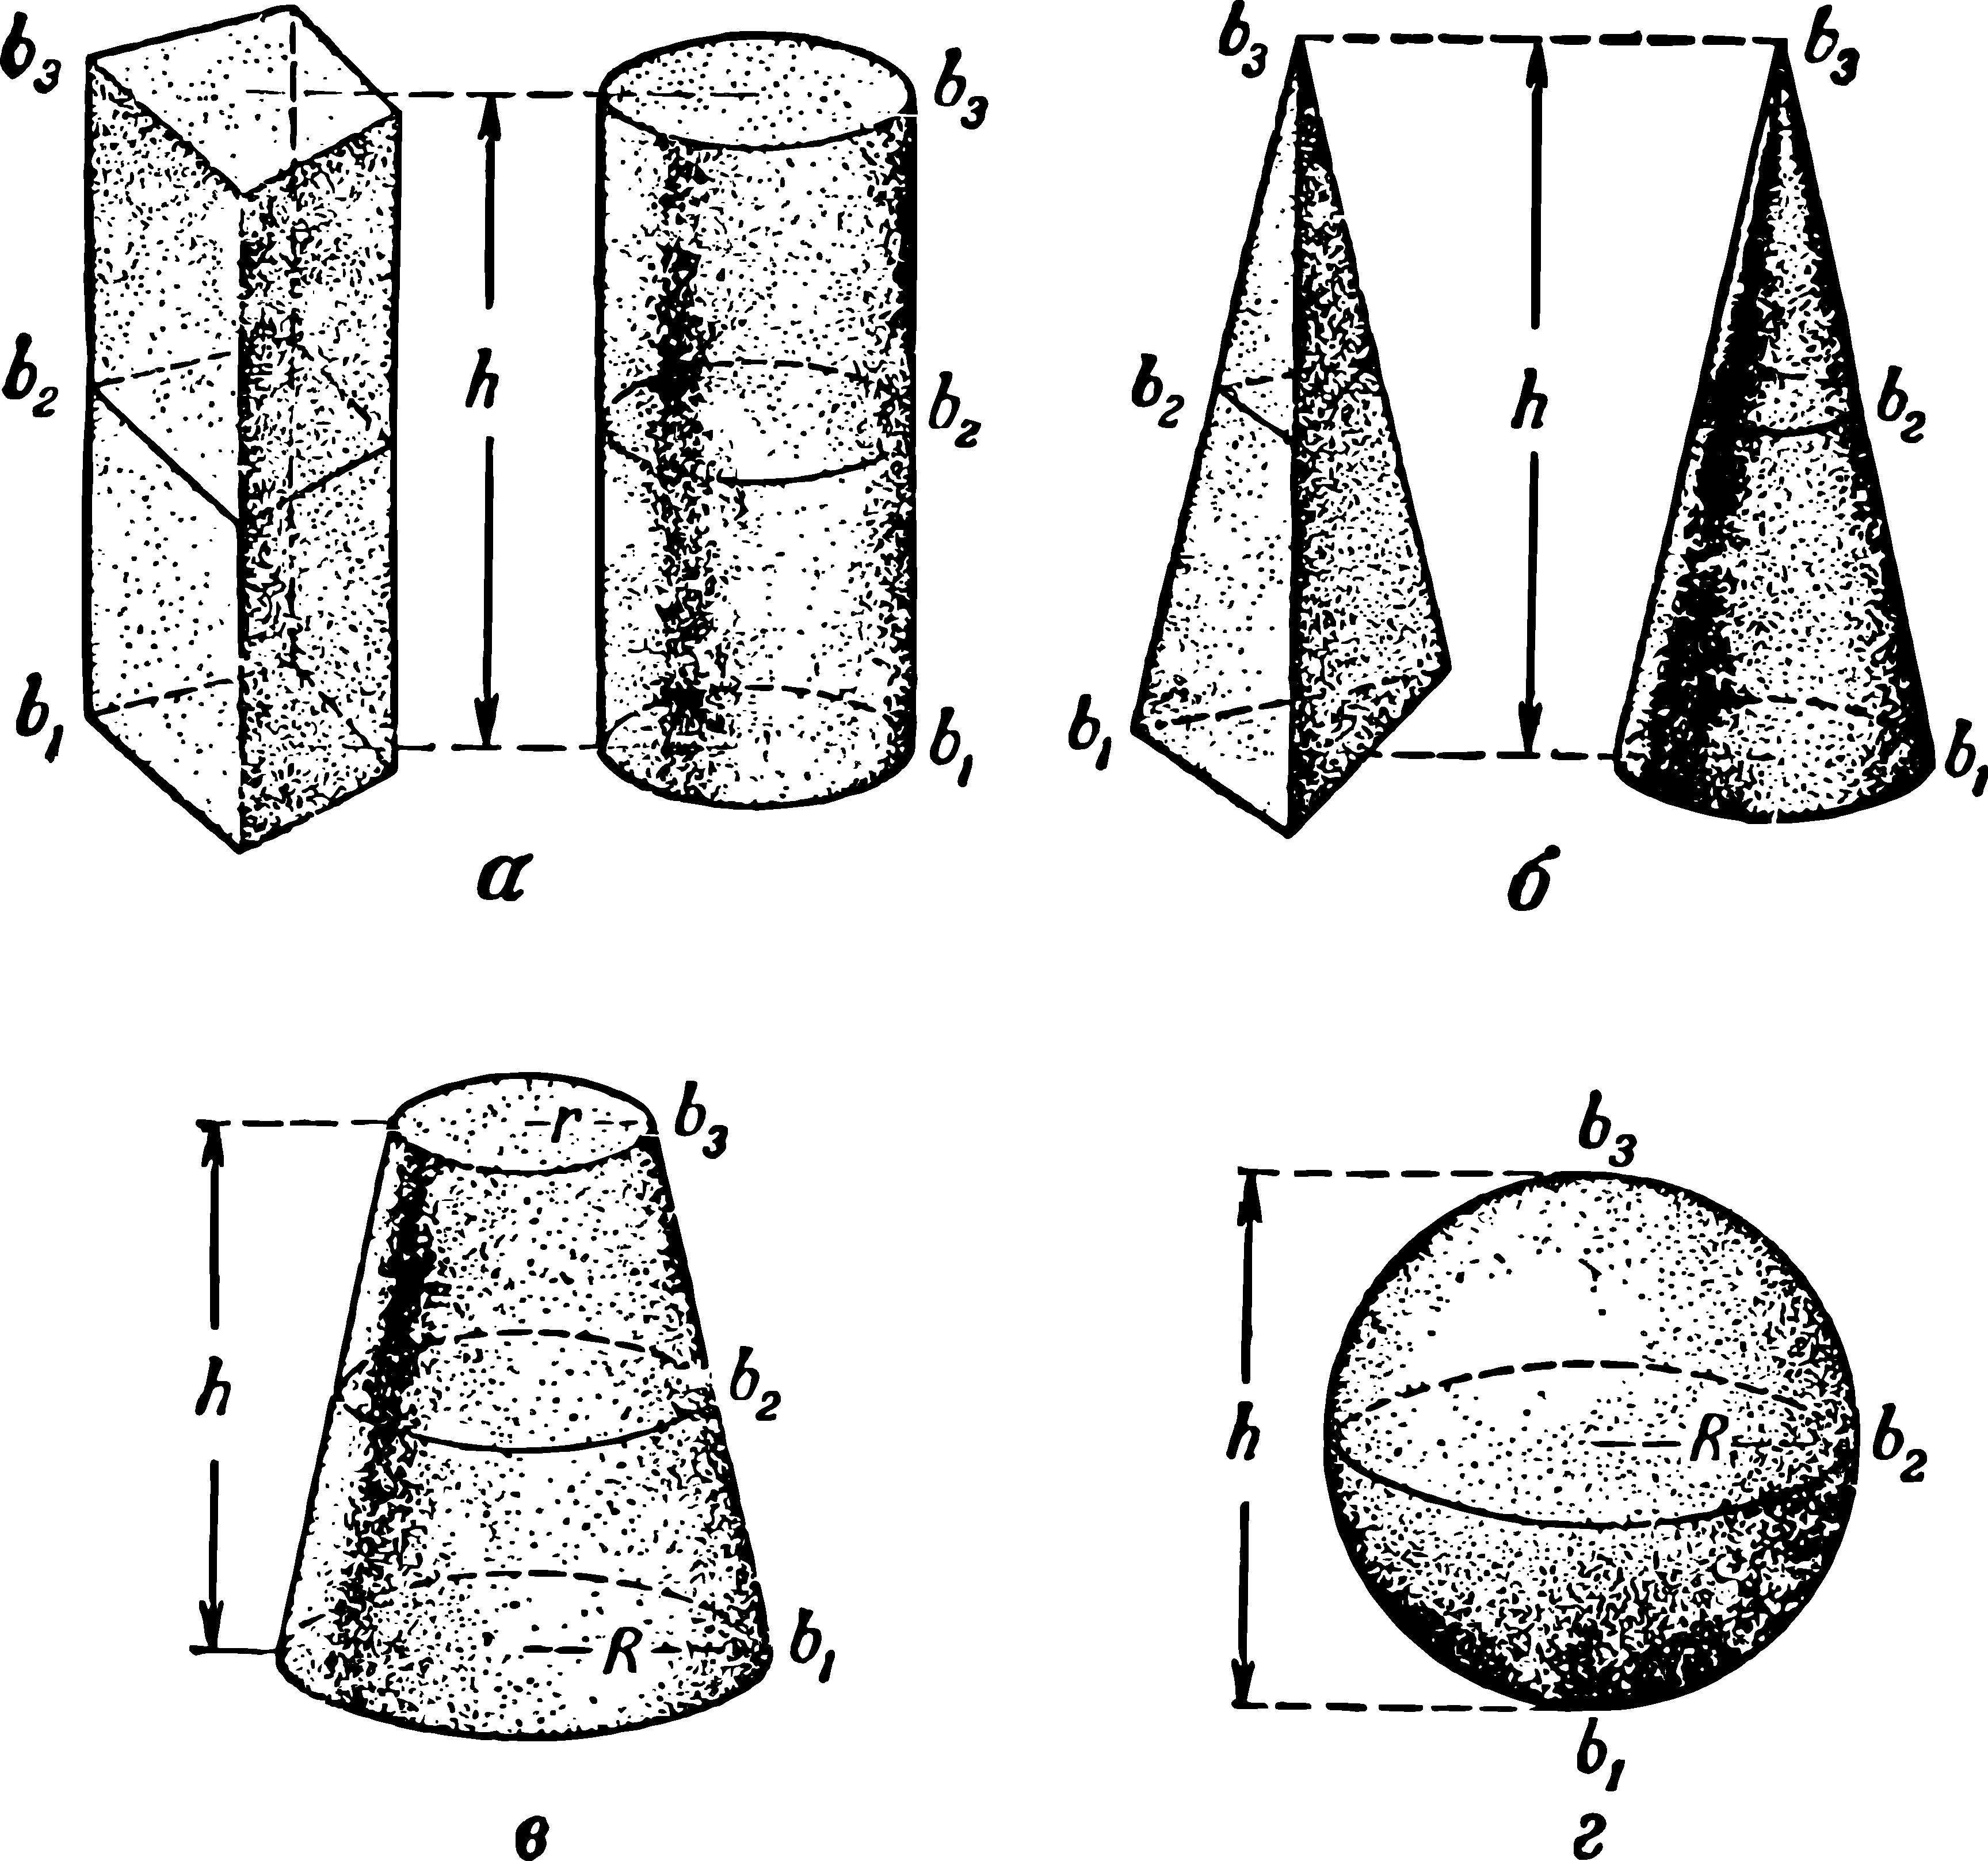
\includegraphics[width=0.9\textwidth]{figures/ch-01/fig-01-17.pdf}
\sidecaption[][-2cm]{Geometric bodies whose volumes can be calculated using a single formula.\label{fig-01-17}}
\end{figure}

\ques Let's note another interesting feature of our universal formula: it is also suitable for calculating the area of plane figures: parallelograms, trapezoids, and triangles, if by 
\begin{enumerate}[label=\textsection]
\item \( h \) we mean, as before, the height of the figure, 
\item by \( b_{1} \) the length of the lower base, 
\item by \( b_{2} \) the length of the middle base and 
\item by $b_{3}$ the length of the lower base. 
\end{enumerate}
How can we confirm this?

\ans Applying the formula, we have: for a parallelogram (square, rectangle) (see \figr{fig-01-18}~\drkgry{a})
\begin{equation*}%
S = \frac{h}{6}\, (b_{1} + 4 b_{1} + b_{1}) = b_{1}h;
\end{equation*}
for a trapezoid (see \figr{fig-01-18}~\drkgry{b})
\begin{equation*}%
S = \frac{h}{6}\, \left( b_{1} + 4 \frac{b_{1} + b_{2}}{2} + b_{3} \right) = \frac{h}{2}\,(b_{1} + b_{3});
\end{equation*}
for a triangle (see \figr{fig-01-18}~\drkgry{c})
\begin{equation*}%
S = \frac{h}{6}\, \left( b_{1} + 4 \frac{b_{1}}{2} + 0 \right) = \frac{b_{1}h}{2}.
\end{equation*}
You can see that our formula has enough right to be called universal.

\begin{figure}[h!]
\centering
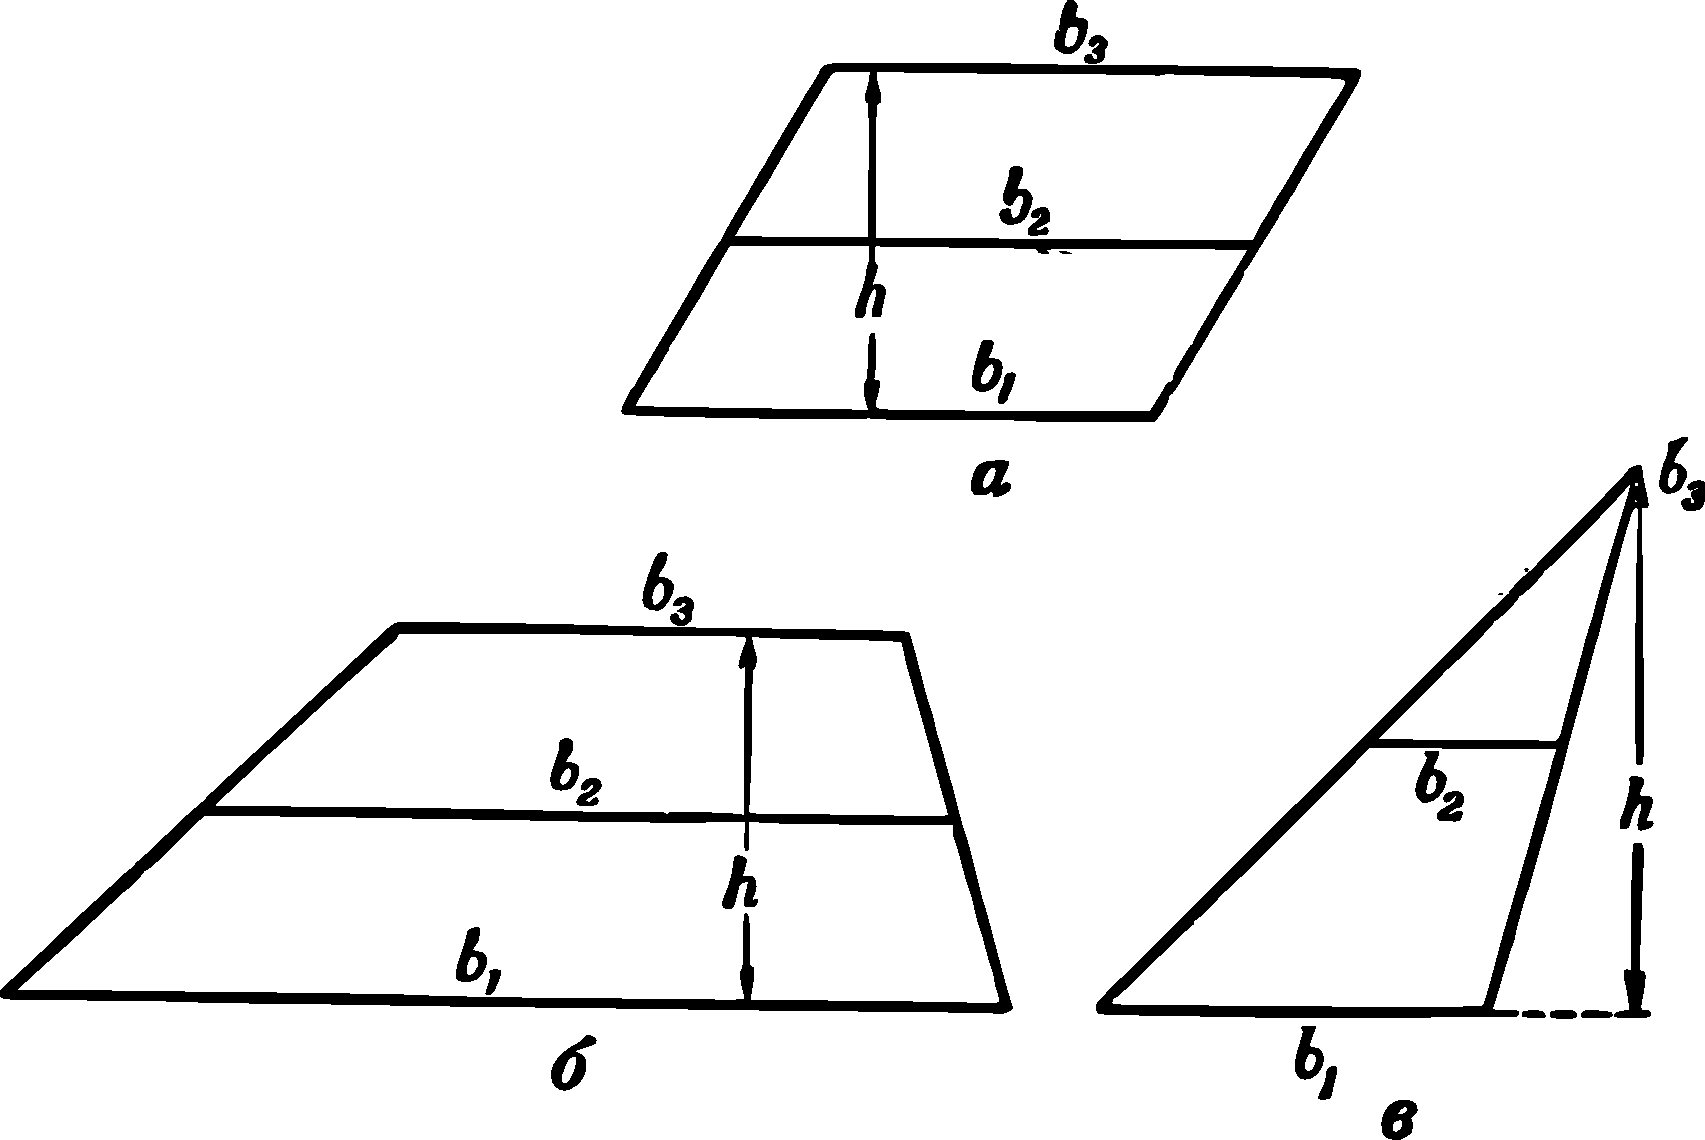
\includegraphics[width=\textwidth]{figures/ch-01/fig-01-18.pdf}
\sidecaption{The universal formula is also suitable for calculating the areas of these figures.\label{fig-01-18}}
\end{figure}


\section{Volume and Weight of a Tree at the Root}
\label{sec-1.12}

So, you have a formula with which you can approximately calculate the volume of a felled tree trunk without worrying about what geometric shape it resembles: a cylinder, a complete cone, or a truncated cone. For this, four measurements are needed -- the length of the trunk and three diameters: the lower cut, the upper, and in the middle of the length. Measuring the lower and upper diameters is very simple; however, determining the average diameter without a special device (``measuring fork'' used by foresters, see \figr{fig-01-19} and \figr{fig-01-20}\sidenote{A similar principle is applied in the well-known device for measuring the diameter of round objects -- the caliper \figr{fig-01-20}, to the right).} is quite difficult. But the difficulty can be overcome by encircling the trunk with a rope and dividing its length by 3 1/7 to get the diameter.

\begin{figure}[h!]
\centering
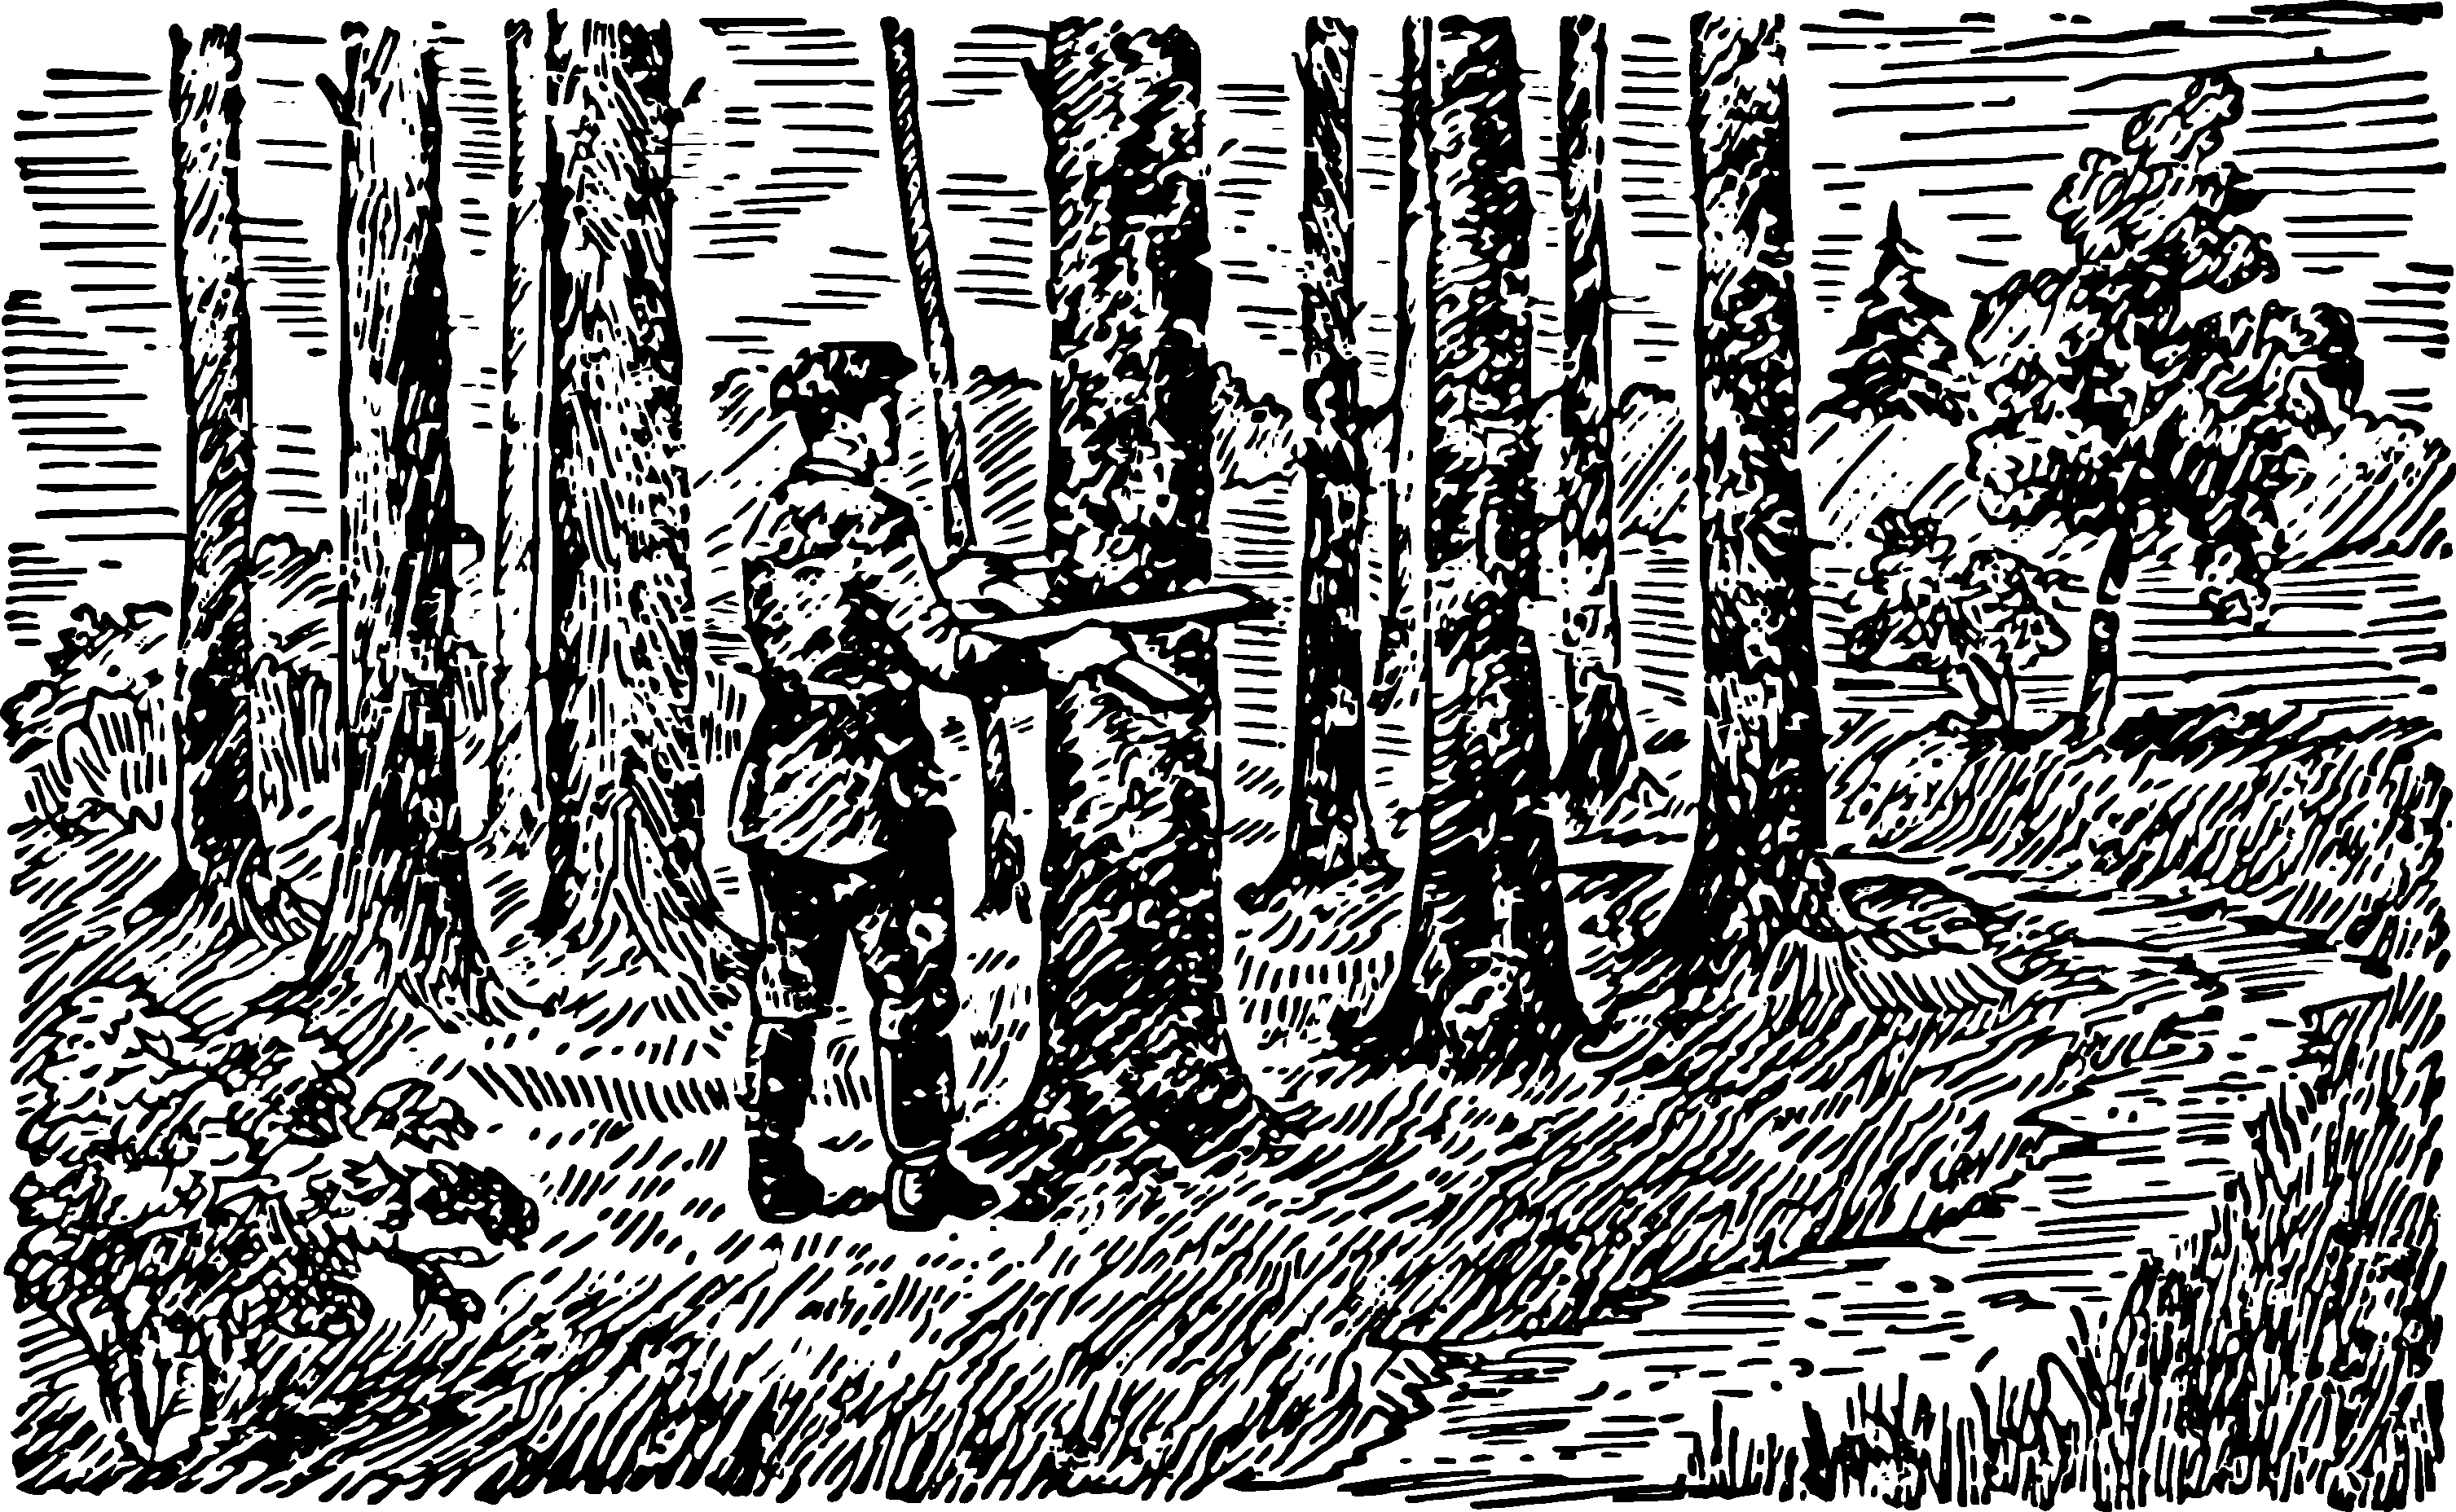
\includegraphics[width=\textwidth]{figures/ch-01/fig-01-19.pdf}
\sidecaption{Measuring the diameter of a tree with a measuring fork.\label{fig-01-19}}
\end{figure}


The volume of a felled tree trunk obtained in this way is accurate enough for many practical purposes. In short, but less accurately, this problem can be solved by calculating the volume of the trunk as the volume of a cylinder, the diameter of the base of which is equal to the diameter of the trunk in the middle of its length; however, the result obtained is underestimated, sometimes by 12\%. But if you mentally divide the trunk into two-meter segments and determine the volume of each of these almost cylindrical parts to then add them up, the result will be much better: it errs on the side of underestimation by no more than 2–3\%.

\begin{figure}[h!]
\centering
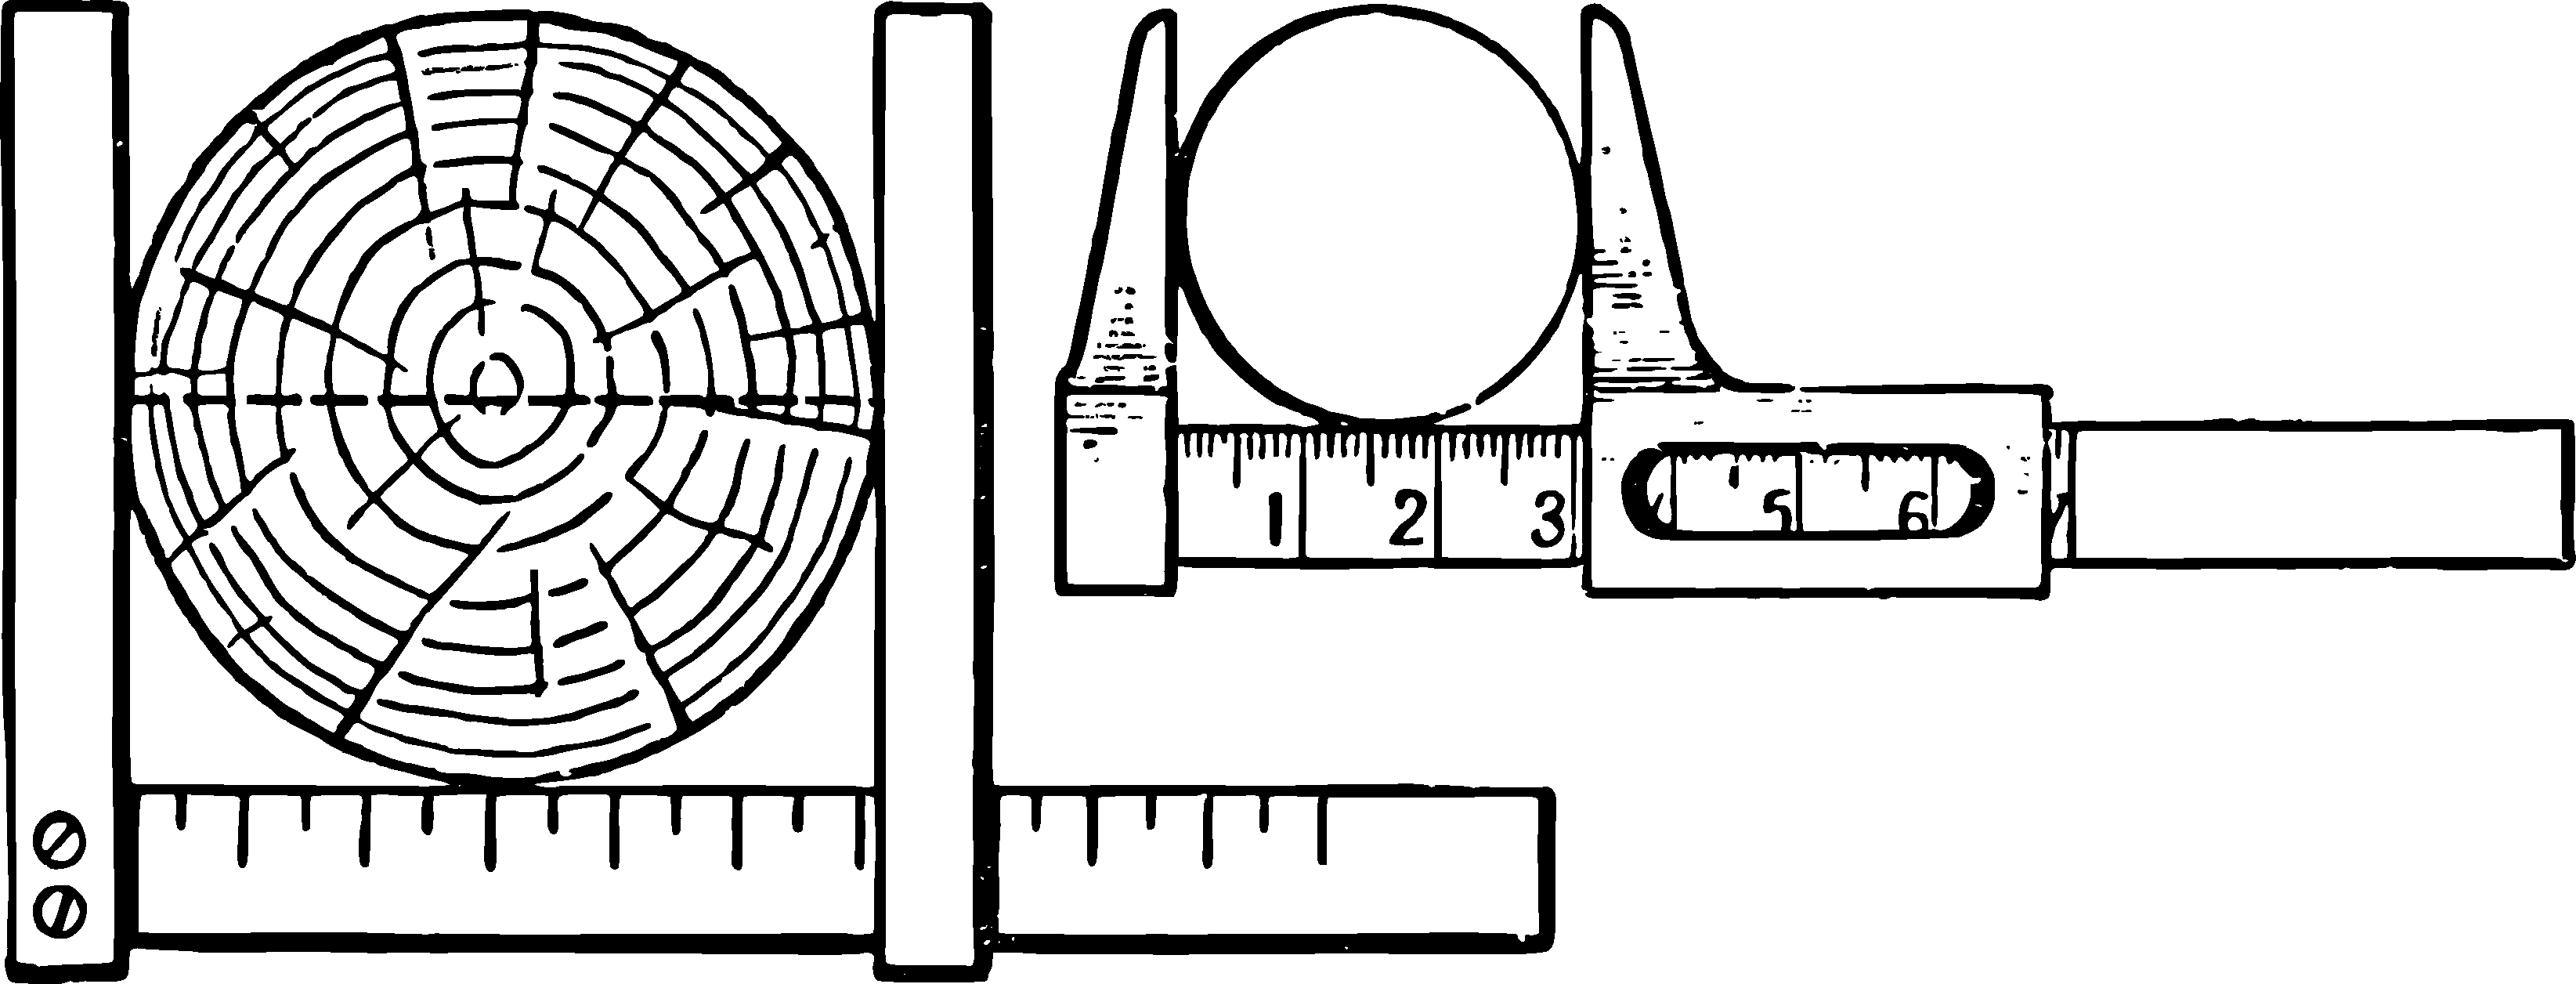
\includegraphics[width=0.9\textwidth]{figures/ch-01/fig-01-20.pdf}
\sidecaption{Measuring fork (left) and caliper (right).\label{fig-01-20}}
\end{figure}

However, all this is completely inapplicable to a tree at the root: if you are not going to climb it, then you can only measure the diameter of its lower part. In this case, to determine the volume, you will have to be satisfied with only a very approximate estimate, comforting yourself with the fact that professional foresters usually proceed in a similar way. They also use a table of so-called ``species numbers,'' i.e., numbers that show what proportion of the volume of the measured tree is compared to the volume of a cylinder of the same height and diameter, measured at the height of a grown man's chest, i.e., 130 cm (this height is the most convenient for measuring). 

\figr{fig-01-21} illustrates this clearly. Of course, ``species numbers'' vary for trees of different species and heights, as the shape of the trunk is variable. However, the fluctuations are not particularly great: for pine and fir trunks (grown in dense plantations), ``species numbers'' range from 0.45 to 0.51, i.e., are approximately half.

\begin{figure}[h!]
\centering
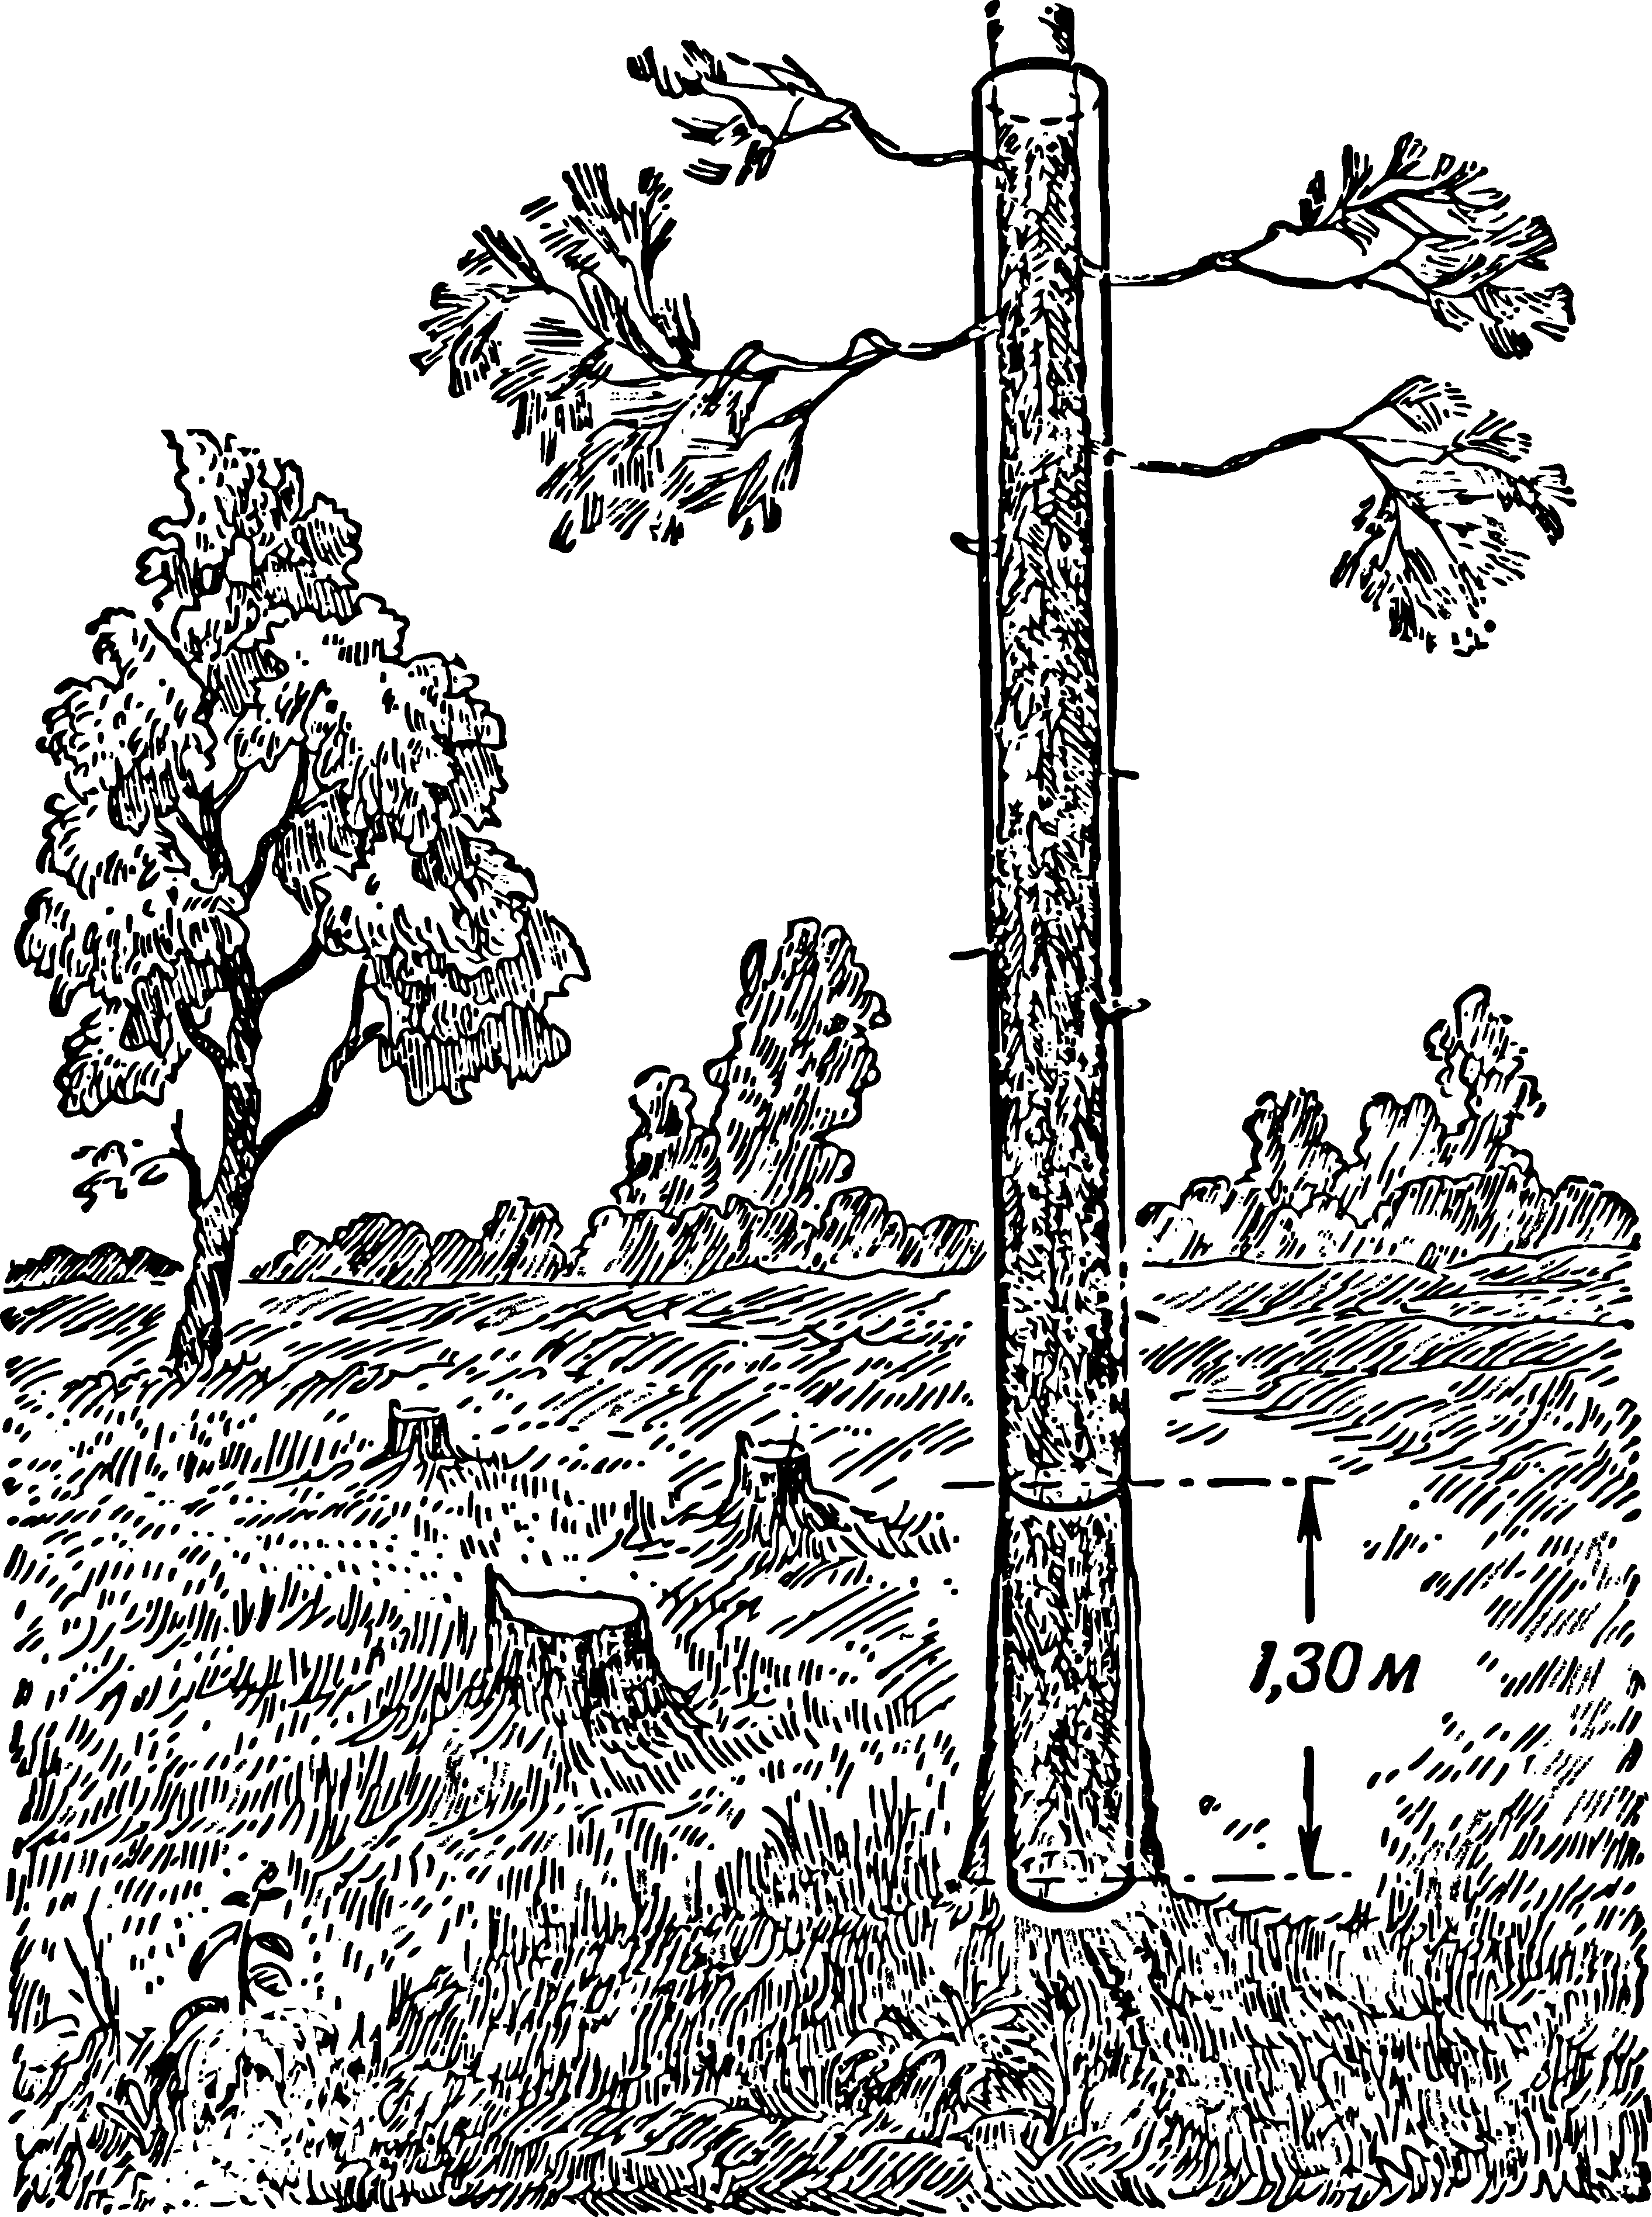
\includegraphics[width=0.8\textwidth]{figures/ch-01/fig-01-21.pdf}
\sidecaption[][-4cm]{What is a ``species number''?\label{fig-01-21}}
\end{figure}

Thus, without much error, it can be assumed that the volume of a coniferous tree at the root is half the volume of a cylinder of the same height with a diameter equal to the diameter of the tree at chest height.

This is, of course, only an approximate estimate, but it is not too far from the true result: up to 2\% in the overestimation direction and up to 10\% in the underestimation direction.\sidenote[][-1cm]{It must be remembered that ``species numbers'' refer only to trees that have grown in the forest, i.e. to tall and thin (smooth, without nodes); for free-standing branched trees, such general rules for calculating volume cannot be specified.}

From here, it is only one step towards estimating the weight of the tree at the root. For this, it is enough to know that 1 cubic meter of fresh pine or fir wood weighs about 600–700 kg. For example, suppose you are standing next to a fir tree, the height of which you have determined to be \SI{28}{\meter}, and the circumference of the trunk at chest height is \SI{120}{\centi\meter}. Then the area of the corresponding circle is \SI{1100}{\centi\meter\squared}, or \SI{0.11}{\meter\squared}, and the volume of the trunk is $1/2 \times 0.11 \times 28 = \SI{1.5}{\meter\cubed}$. Assuming that 1 cubic meter of fresh fir wood weighs on average \SI{650}{\kilo\gram}, we find that 1.0 cubic meter should weigh about a ton (\SI{1000}{\kilo\gram}).


\section{Leaf Geometry}
\label{sec-1.12}

\ques In the shadow of a silver poplar from its roots, a thicket has grown. Pick a leaf and notice how large it is compared to the leaves of the parent tree, especially those that grew in bright sunlight. The shaded leaves compensate for the lack of light with the size of their area, capturing sunlight rays. Understanding this is the task of botany. But the geometer can also have a say here: he can determine exactly how many times the area of the thicket leaf is larger than the area of the parent tree leaf.

How would you solve this problem?


\ans You can go two ways. First, determine the area of each leaf separately and find their ratio. The area of the leaf can be measured by covering it with transparent grid paper, each square of which corresponds, for example, to 4 square millimeters (a sheet of transparent grid paper used for this purpose is called a pallet). This is a perfectly correct but overly laborious method.\sidenote{However, this method has an advantage: using it, you can compare the areas of leaves with different shapes, which cannot be done according to the method described below.}

A shorter method is based on the fact that both leaves, different in size, still have the same or almost the same shape: in other words, they are geometrically similar figures. We know that the areas of such figures are related as the squares of their linear dimensions. Therefore, by determining how many times one leaf is longer or wider than the other, we can find the ratio of their areas simply by squaring this number. Let the thicket leaf be 15 cm long, and the leaf from the tree branch only 4 cm long; the ratio of their linear dimensions is 15/4, and therefore, in terms of area, one is larger than the other by 225/16 times, or about 14. Rounding off (since full accuracy cannot be achieved here), we can say that the thicket leaf is approximately 15 times larger than the tree leaf in terms of area.

Let us consider another example.
%\clearpage

\ques At a dandelion grown in shade, a leaf is 31 cm long. At another specimen grown in sunlight, the leaf blade is only 3.3 cm long. Approximately how many times is the area of the first leaf larger than the area of the second?



\ans We proceed as before. The ratio of the areas is
\begin{equation*}%
\frac{31^{2}}{3.3^{2}} = \frac{960}{10.9} = 87;
\end{equation*}
so one leaf is approximately 90 times larger than the other in terms of area.

\begin{marginfigure}[-3.5cm]%[h!]
\centering
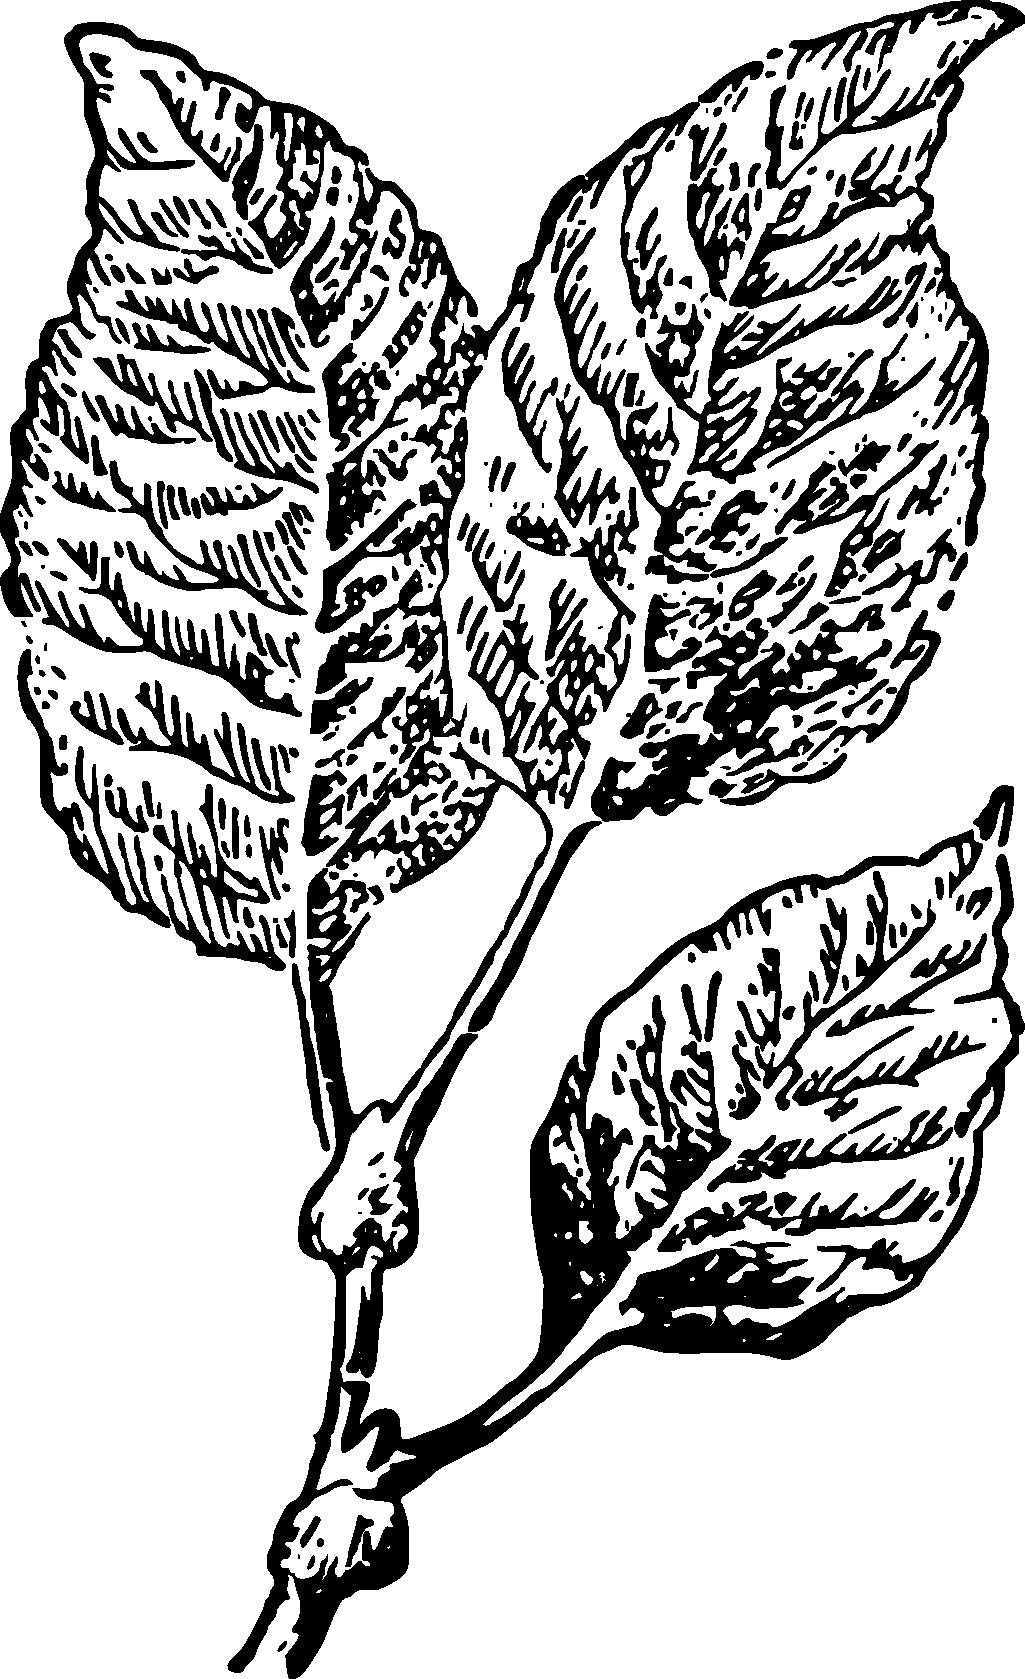
\includegraphics[width=0.9\textwidth]{figures/ch-01/fig-01-22.pdf}
\sidecaption{Determine the ratio of the areas of these leaves.\label{fig-01-22}}
\end{marginfigure}


It is easy to find in the forest many pairs of leaves of the same shape but different sizes, thus providing interesting material for geometric problems on the ratio of areas of similar figures. It always seems strange to an unaccustomed eye that a relatively small difference in the length and width of leaves results in a noticeable difference in their areas. For example, if two leaves, geometrically similar in shape, differ in length by 20\%, then the ratio of their areas is 
\begin{equation*}%
1.2^{2} \approx 1.4, 
\end{equation*}
meaning the difference is 40\%. And with a difference in width of 40\%, One leaf exceeds the other in area by 
\begin{equation*}%
1.4^{2} \approx 2, 
\end{equation*}
or nearly twice.

\ques  We invite the reader to determine the ratio of the areas of the leaves depicted in \figr{fig-01-22} and \figr{fig-01-23}.

\begin{marginfigure}[-4.5cm]%[h!]
\centering
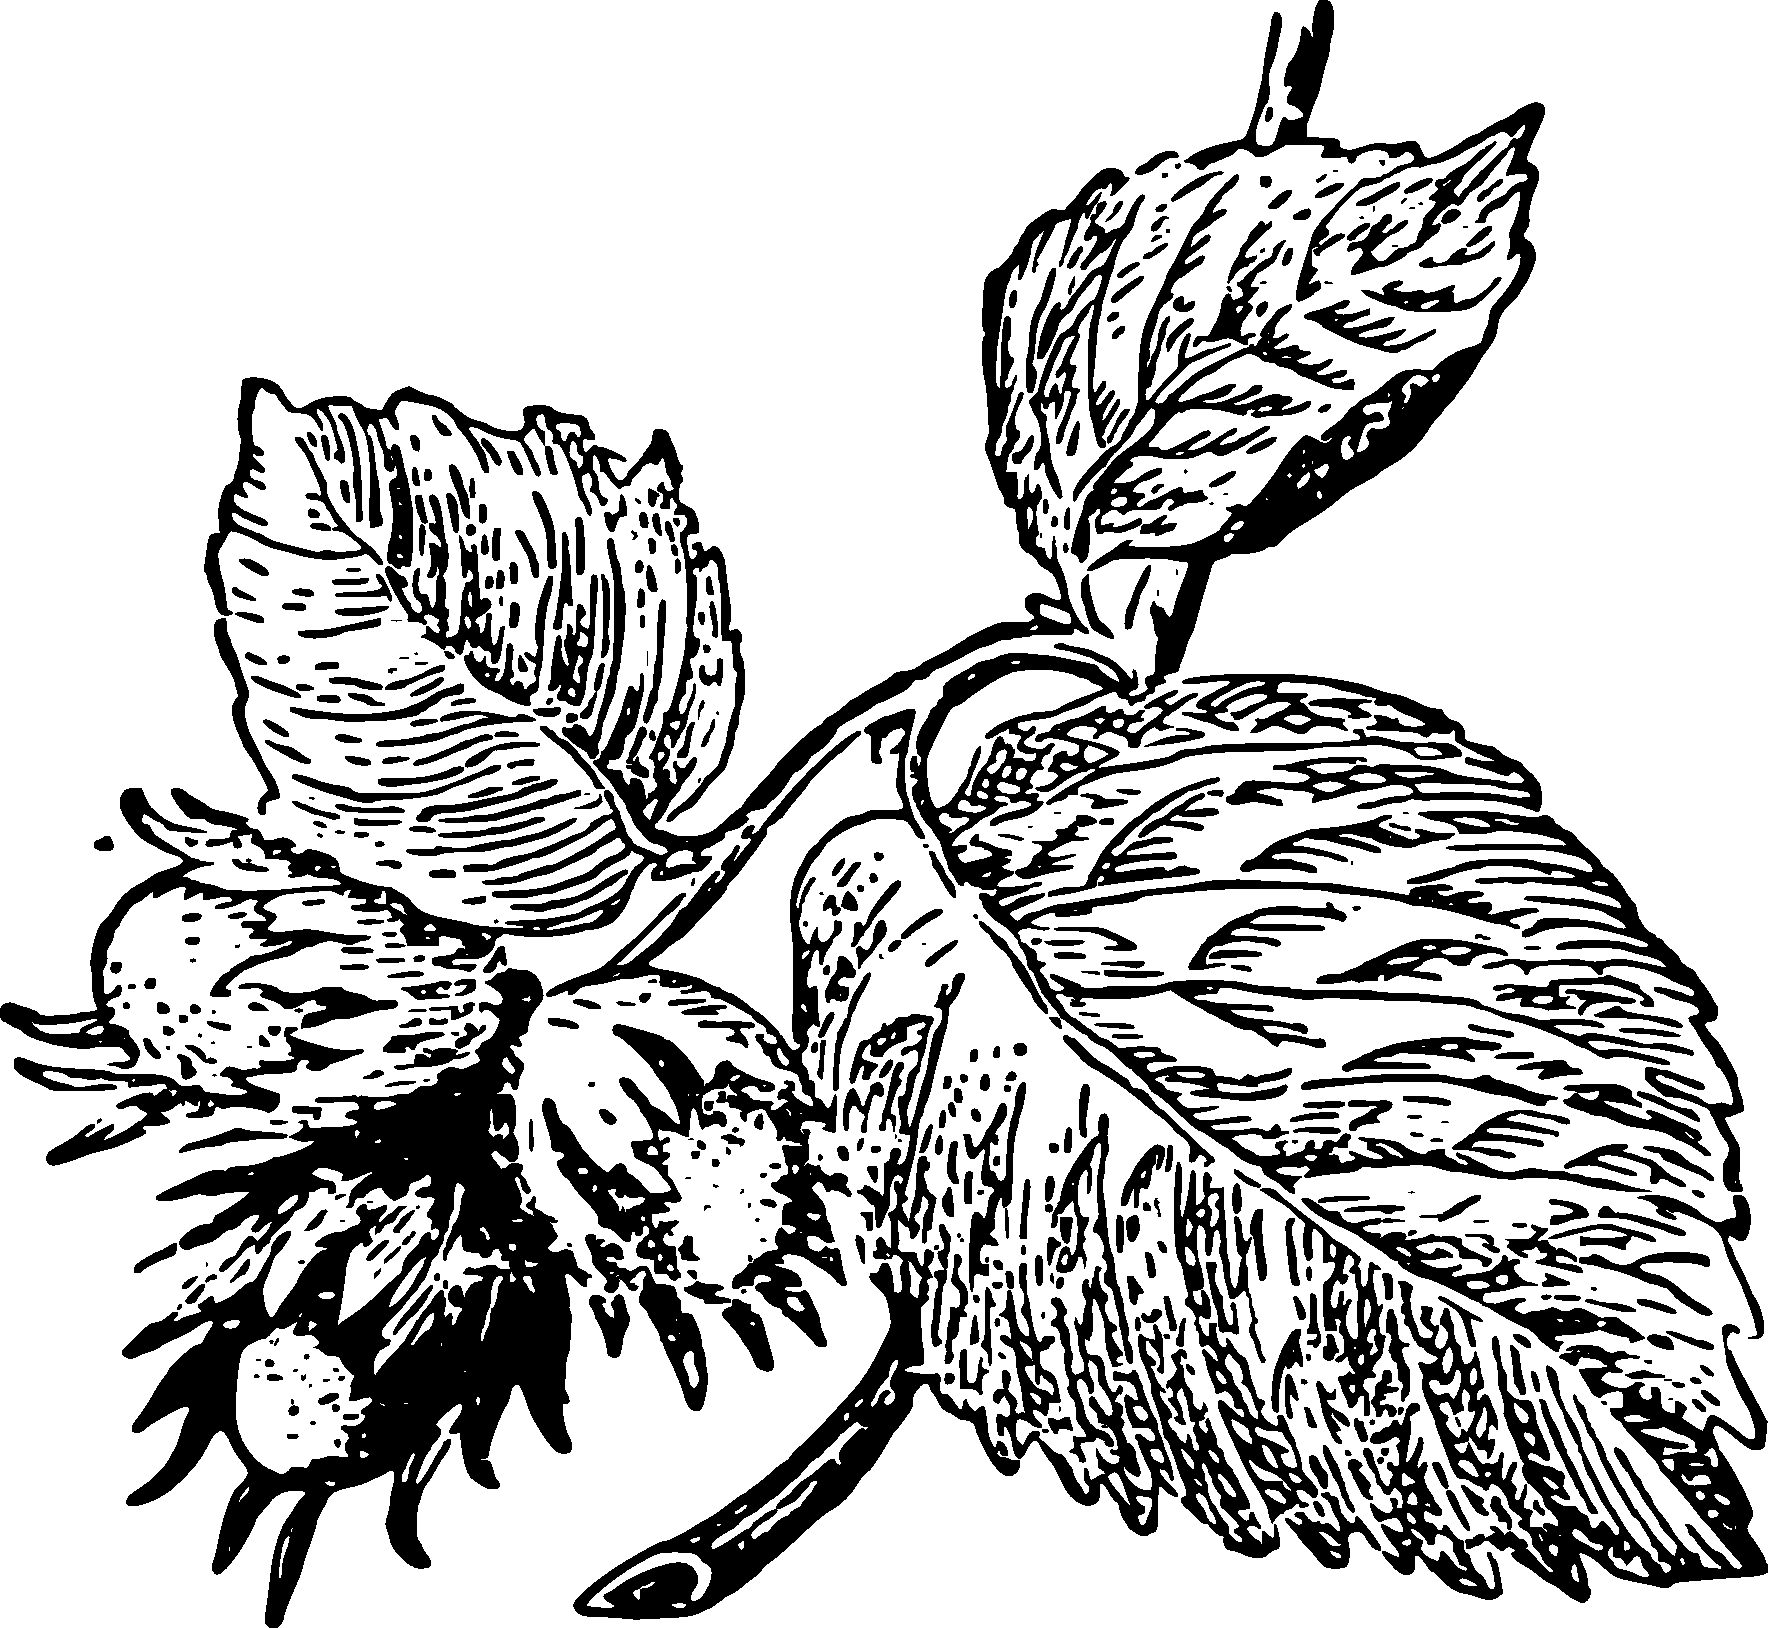
\includegraphics[width=0.9\textwidth]{figures/ch-01/fig-01-23.pdf}
\sidecaption{Determine the ratio of the areas of these leaves.\label{fig-01-23}}
\end{marginfigure}


%\ques \textsf{\small\color{Salmon} We invite the reader to determine the ratio of the areas of the leaves depicted in \figr{fig-01-22}and \figr{fig-01-23}.}

\section{Six-legged heroes}
\label{sec-1.14}

Amazing creatures, ants! Swiftly climbing up stems with a burden much heavier than their tiny size (\figr{fig-01-24}), ants present an intriguing puzzle to observant individuals: where does the insect derive the strength to effortlessly carry a load ten times its own weight? Indeed, a human might struggle to climb stairs while carrying, for instance, a piano (\figr{fig-01-24}), with the weight ratio of the load to the body being roughly similar to that of an ant. Thus, it seems that the ant is relatively stronger than a human!

But is it really so?

Without geometry, this cannot be understood. Let's listen to what the expert (Professor A.F. Brandt) has to say, primarily about the strength of muscles, and then about the current question regarding the comparison of forces between the insect and the human: ``A muscle resembles a resilient cord; however, its contraction is based not on elasticity, but on other reasons, and is normally manifested under the influence of nervous excitation, as demonstrated in physiological experiments involving the application of electric current to the corresponding nerve or directly to the muscle.''

``These experiments are easily conducted on muscles excised from a freshly killed frog, as the muscles of cold-blooded animals retain their vital properties for a long time even outside the organism, even at ordinary temperatures. The experiment is very simple. The main calf muscle, which extends the hind leg, is excised together with a piece of the femur bone from which it originates, and together with the terminal tendon. This muscle is found to be the most convenient due to its size, shape, and ease of preparation. A hook is passed through the tendon, and a weight is attached to it.'' 

\begin{marginfigure}[-3cm]%[h!]
\centering
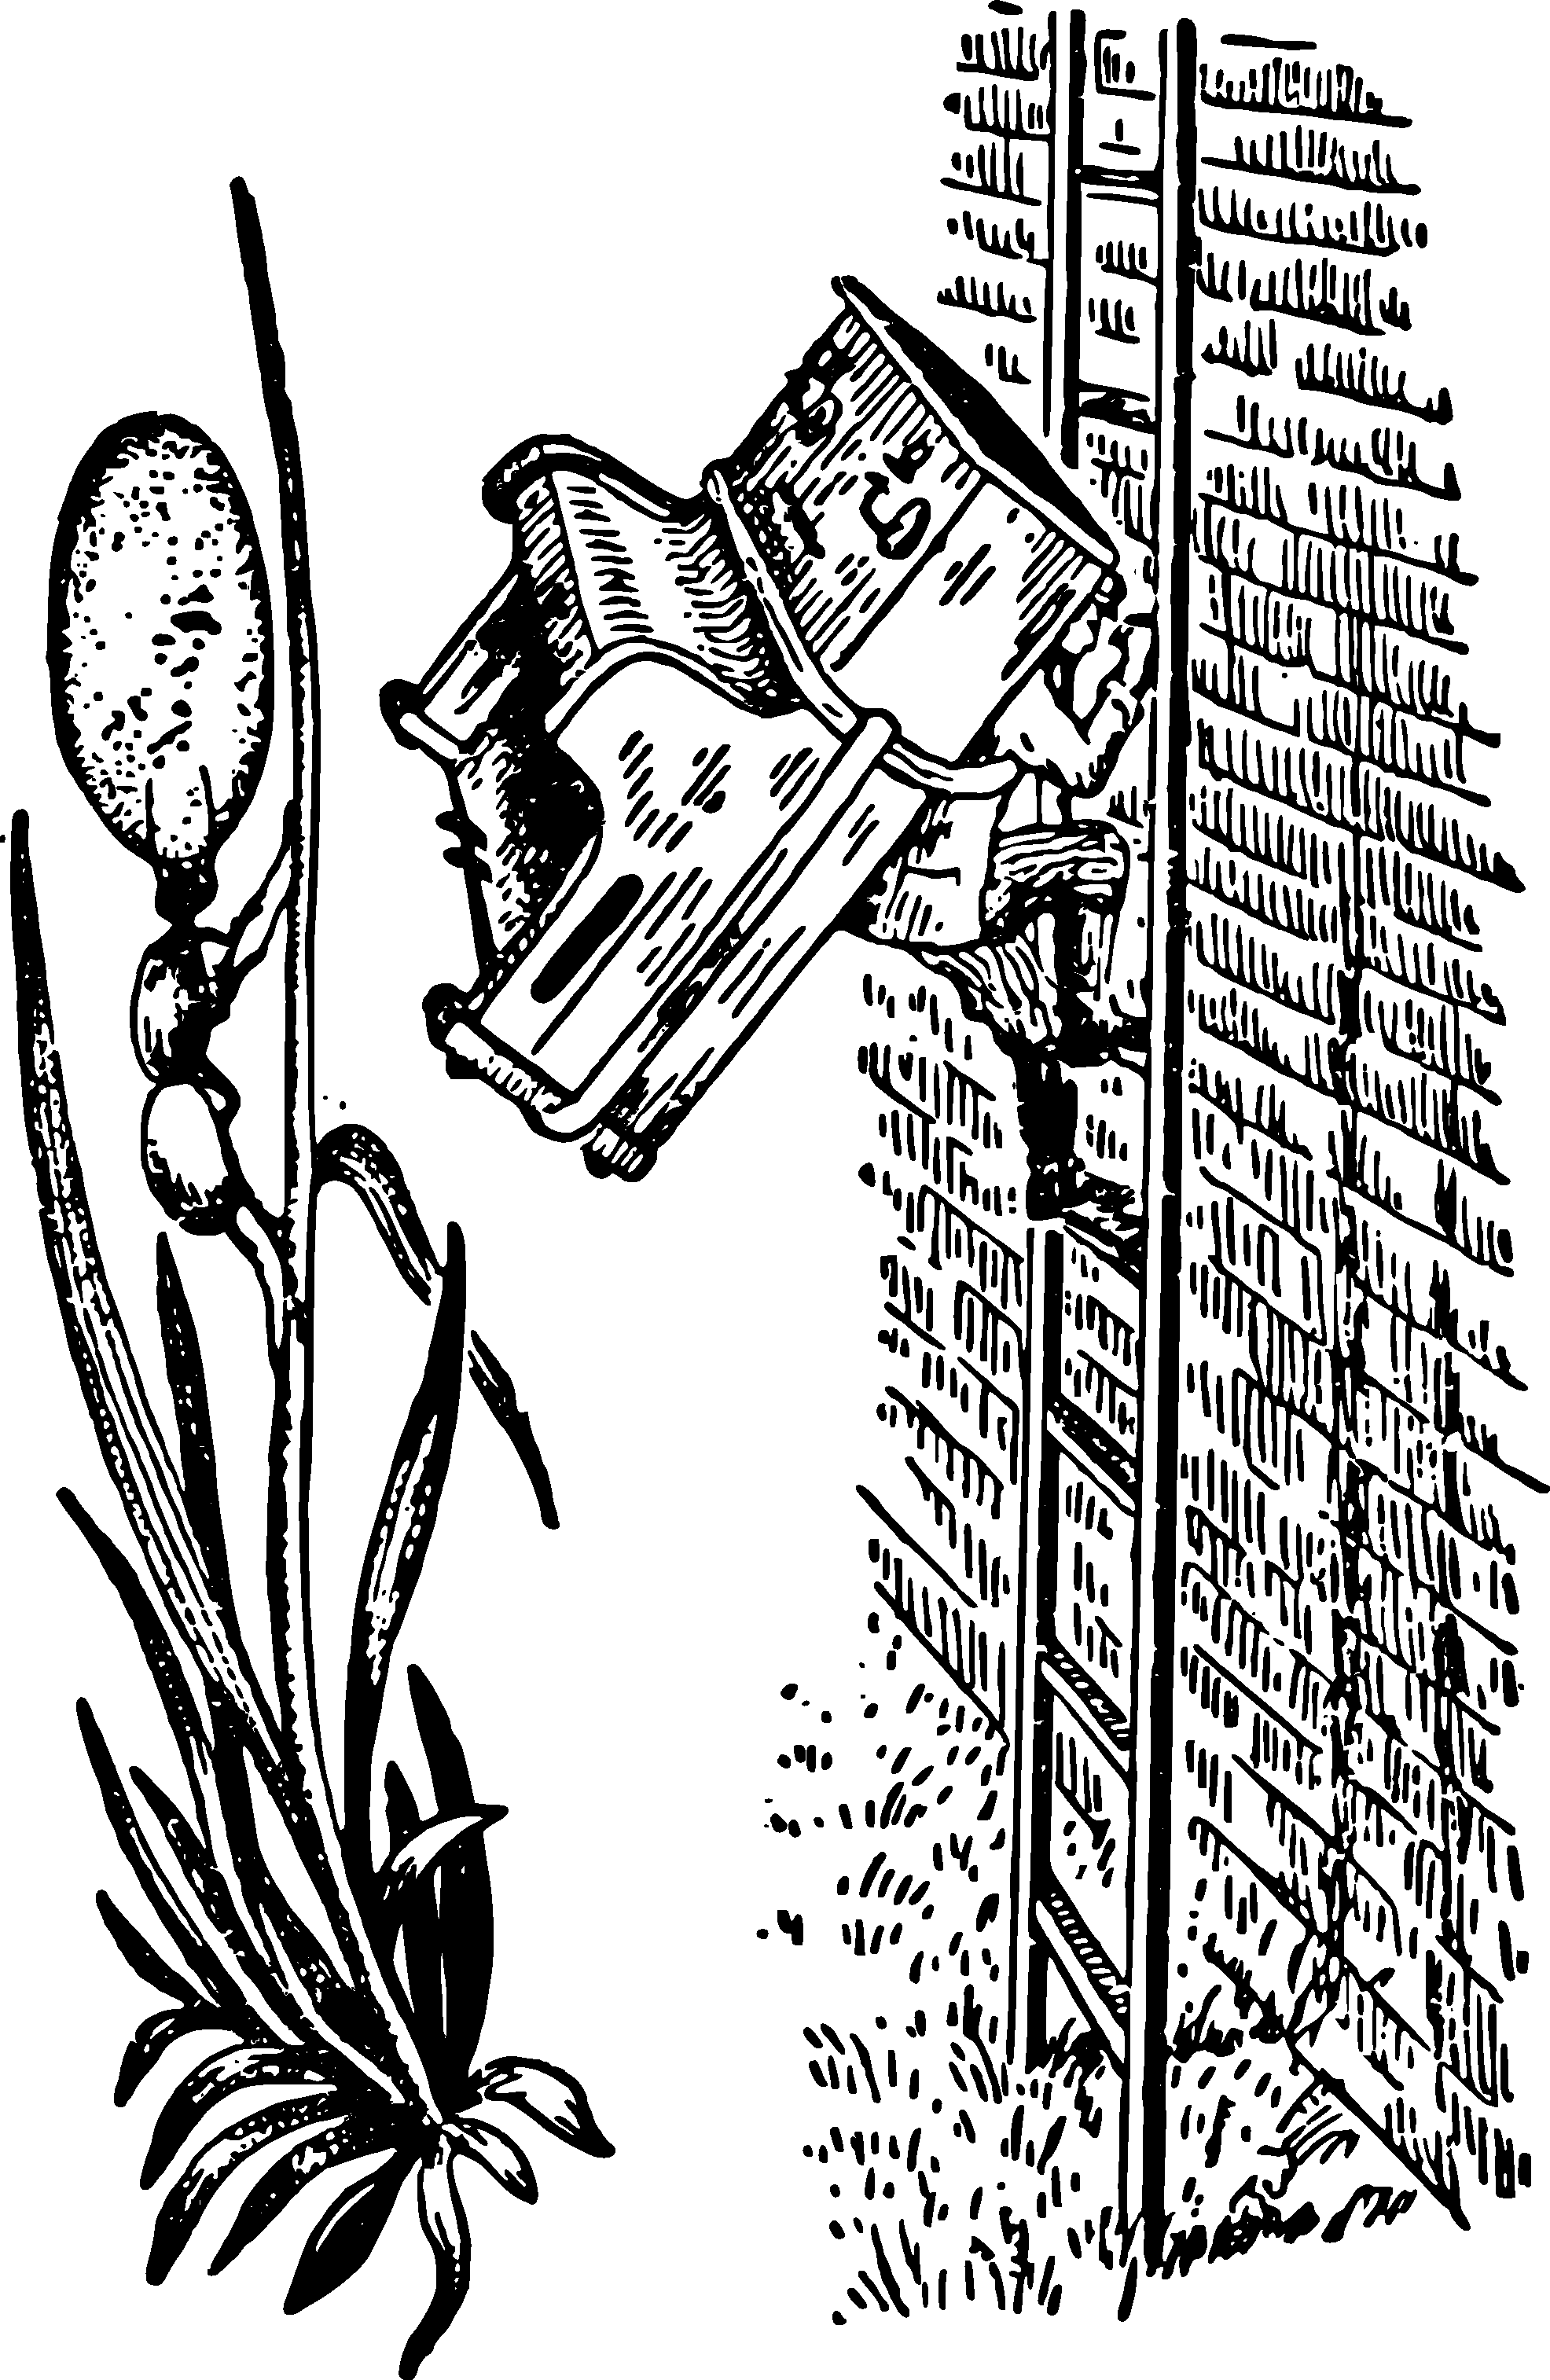
\includegraphics[width=\textwidth]{figures/ch-01/fig-01-24.pdf}
\sidecaption{The six-legged hero.\label{fig-01-24}}
\end{marginfigure}


``If wires from a galvanic element are touched to such a muscle, it instantly contracts, shortens, and lifts the load. By gradually adding additional weights, the maximum lifting capacity of the muscle can be easily determined. Now, if we bind together in length two, three, or four identical muscles and stimulate them simultaneously, we will not achieve greater lifting force; the load will only be lifted to a greater height, corresponding to the sum of the contractions of individual muscles. However, if we bundle two, three, or four muscles together, the entire system will lift a weight many times greater when stimulated. The same result, obviously, would be obtained if the muscles were fused together. Thus, we conclude that the lifting force of muscles depends not on their length or total mass, but only on their thickness, i.e., \emph{cross-sectional area}.''

``After this digression, let's turn to the comparison of similarly structured, geometrically similar, but differently sized animals. Let's imagine two animals: the original and one that has been doubled in size in all linear dimensions. In the second animal, the volume and weight of the entire body, as well as each of its organs, will be eight times greater; however, all corresponding planar dimensions, including the cross-sectional area of muscles, will be only four times greater. It turns out that as the animal grows to twice the length and eight times the weight, its muscular strength increases only fourfold, i.e., the animal becomes relatively weaker. Based on this reasoning, an animal that is three times longer (with cross-sectional areas three times larger and a weight 27 times greater) would be relatively three times weaker, and one that is four times longer would be four times weaker, and so on.''

``The law of unequal growth in volume and weight of the animal, and thus of muscular strength, explains why insects -- as observed in ants, predatory wasps, and others -- can carry loads 30 to 40 times their own weight, whereas a human can typically carry excluding gymnasts and porters -- only about 9/10 times their own weight, -- and a horse, which we view as a magnificent living work machine, even less, namely, only about 7/10 of its own weight.''\sidenote{For more details, see \emph{Fun with Physics} by Ya. I. Perelman, Chapter X \emph{Mechanics in the Living World}.}

After these explanations, we will look at the feats of that ant-giant with different eyes, about whom I.A. Krylov mockingly wrote:
\begin{quote}
\emph{Some ant had extraordinary strength,\\
 Such as was unheard of even in ancient times; \\
 He even (says his faithful historian)\\
 Could lift two barley grains.}
\end{quote} 


\begin{center}
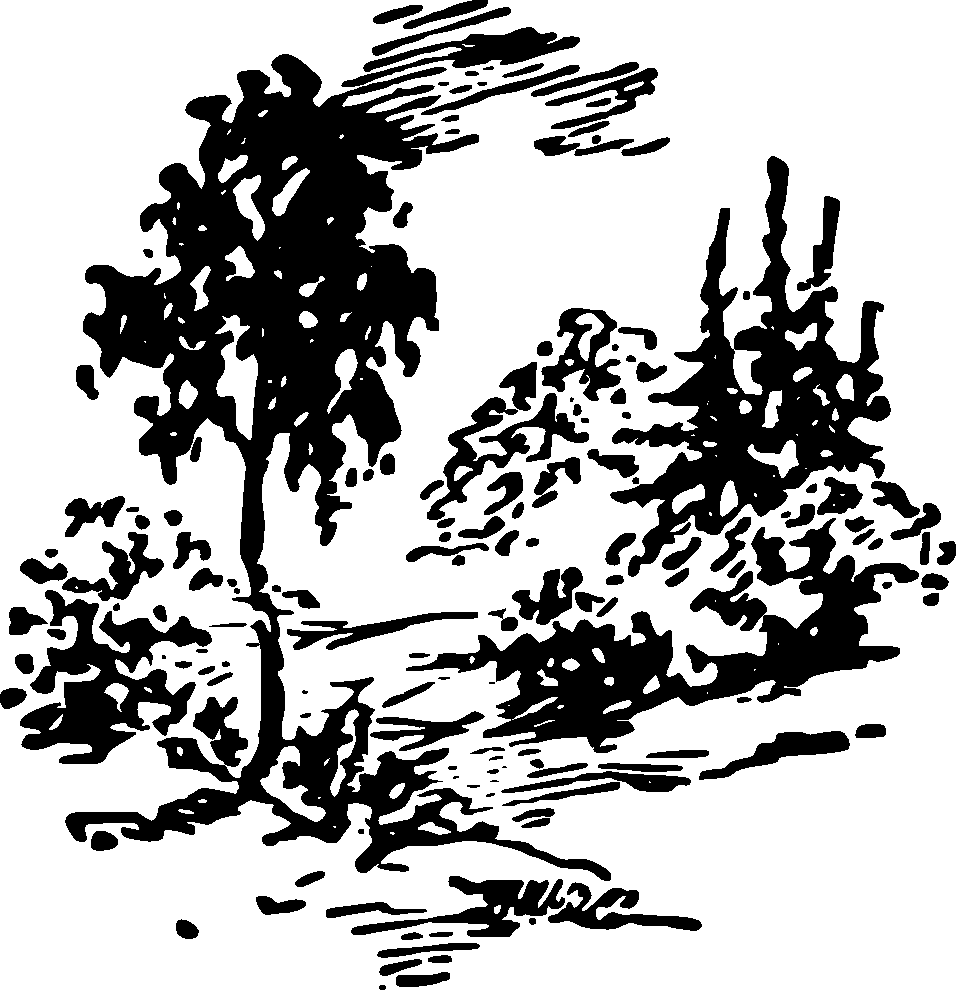
\includegraphics[width=0.3\textwidth]{figures/ch-01/fig-ch-01-tail.pdf}
\end{center}





















\end{document}
%%% Local Variables:
%%% mode: latex
%%% TeX-master: t
%%% End:
